%------------------------------------------------------------------------
%- Reference for the EALib, addition Array                              -
%------------------------------------------------------------------------
%- History of modification                                              -
%-                                                                      -
%-  ver.1.01 : 2000/05/29 Ruediger Alberts (Institut fuer               -
%-                        Neuroinformatik, Bochum)                      -
%-               original                                               -
%-  ver.1.02 : 2001/01/04 Tatsuya Okabe (HONDA R&D EUROPE DEUTSCHLAND)  -
%-               separate files , add index                             -
%-  ver.1.03 : 2001/01/30 Tatsuya Okabe (HONDA R&D EUROPE DEUTSCHLAND)  -
%-               include some classes about random generator            -
%-  ver.1.04 : 2001/02/05 Tatsuya Okabe (HONDA R&D EUROPE DEUTSCHLAND)  -
%-               include some important classes                         -
%-  ver.1.10 : 2001/02/14 Tatsuya Okabe (HONDA R&D EUROPE DEUTSCHLAND)  -
%-               release version                                        -
%-  ver.1.11 : 2001/06/08 Tatsuya Okabe (HONDA R&D EUROPE DEUTSCHLAND)  -
%-               correct some mistakes                                  -
%-  ver.1.12 : 2002/05/22 Ruediger Alberts (ZN AG, Bochum)              -
%-               splitted parts for EALib, Array and Rng                -
%-                                                                      -
%-  ver.1.13 :                                                          -
%-                                                                      -
%-  ver.1.14 :                                                          -
%-                                                                      -
%-  ver.1.15 :                                                          -
%-                                                                      -
%------------------------------------------------------------------------

\documentclass{report}
\usepackage{a4}
\usepackage{graphicx}
\usepackage{makeidx}
\makeindex
% =======================================================================
% Dateiname:        Vorlage.tex
% Autor:            Ruediger Alberts
% EMail:            Ruediger.Alberts@neuroinformatik.ruhr-uni-bochum.de
% Erstellt am:      1999-09-07
% Letzte Aenderung: 1999-09-09
%
% Datei wird mit Befehl ``% =======================================================================
% Dateiname:        Vorlage.tex
% Autor:            Ruediger Alberts
% EMail:            Ruediger.Alberts@neuroinformatik.ruhr-uni-bochum.de
% Erstellt am:      1999-09-07
% Letzte Aenderung: 1999-09-09
%
% Datei wird mit Befehl ``% =======================================================================
% Dateiname:        Vorlage.tex
% Autor:            Ruediger Alberts
% EMail:            Ruediger.Alberts@neuroinformatik.ruhr-uni-bochum.de
% Erstellt am:      1999-09-07
% Letzte Aenderung: 1999-09-09
%
% Datei wird mit Befehl ``\input{Vorlage}'' in LaTex-Dokumente 
% (Latex2Epsilon) eingebunden und stellt Befehle zur einfachen Doku- 
% mentation von C-Funktionen/C++-Methoden bereit.
% =======================================================================

\usepackage{ifthen}

    % Definition von Konstanten:
    \newcommand{\ParamDelim}            % Trennungstext zwischen
        { \ - }                         % Parametername und -beschreibung.
    \newcommand{\NormMethodEnd}         % Endtext von Methode bei 
        {\ \ );}                        % veraenderbarer Aufrufinstanz.
    \newcommand{\ConstMethodEnd}        % Endtext von Methode bei
        {\ \ ) const;}                  % nicht veraenderbarer Aufrufinstanz.
    \newcommand{\MaxLabelTxt}           % Komponentenbeschreibungstext
        {{\bf Besonderheiten: }}        % mit maximaler Breite.
    \newcommand{\MethodBegin}           % Beginntext einer Methode.
        {(\ }
    \newcommand{\InBetween}             % Text zwischen Rueckgabewert und
        {\ \ }                          % Methodenname.

    % Definition eigener Variablen:


    \newboolean{ConstInstance}          % Gibt an, ob die Instanz, die
                                        % die Methode aufruft veraendert
                                        % werden darf oder nicht. Im
                                        % 2. Fall endet die Methode mit
                                        % ``) const;'', im 1. Fall 
                                        % mit ``);''.
    \newcounter{SavedParams}            % Anzahl der gespeicherten
                                        % Parameter.
    \setcounter{SavedParams}{0}
    \newcommand{\ParamOne}{}            % Definition der 10 
    \newcommand{\ParamTypeOne}{}        % abspeicherbaren Parameter,
    \newcommand{\ParamDescrOne}{}       % ihrer Typen und Beschreibungen.
    \newcommand{\ParamTwo}{}            
    \newcommand{\ParamTypeTwo}{}
    \newcommand{\ParamDescrTwo}{}
    \newcommand{\ParamThree}{}
    \newcommand{\ParamTypeThree}{}
    \newcommand{\ParamDescrThree}{}
    \newcommand{\ParamFour}{}
    \newcommand{\ParamTypeFour}{}
    \newcommand{\ParamDescrFour}{}
    \newcommand{\ParamFive}{}
    \newcommand{\ParamTypeFive}{}
    \newcommand{\ParamDescrFive}{}
    \newcommand{\ParamSix}{}
    \newcommand{\ParamTypeSix}{}
    \newcommand{\ParamDescrSix}{}
    \newcommand{\ParamSeven}{}
    \newcommand{\ParamTypeSeven}{}
    \newcommand{\ParamDescrSeven}{}
    \newcommand{\ParamEight}{}
    \newcommand{\ParamTypeEight}{}
    \newcommand{\ParamDescrEight}{}
    \newcommand{\ParamNine}{}
    \newcommand{\ParamTypeNine}{}
    \newcommand{\ParamDescrNine}{}
    \newcommand{\ParamTen}{}
    \newcommand{\ParamTypeTen}{}
    \newcommand{\ParamDescrTen}{}
    \newlength{\MaxParamWidth}          % Breite des breitesten 
                                        % Methodenparameters.
    \newlength{\SpecialWidth}           % Breite des Textes 
    \settowidth{\SpecialWidth}          % {\bf Besonderheiten}.
        {\MaxLabelTxt}
    \newlength{\ParamDelimWidth}        % Breite des Textes `` \ - ``.
    \settowidth{\ParamDelimWidth}
        {\ParamDelim}
    \newlength{\ParamDescrWidth}        % Max. Breite des Parametertextes.
    \newlength{\SpecialRetTxtWidth}     % Max. Breite der Texte fuer
                                        % Besonderheiten und Rueckgabewert.
    \newlength{\MethodBeginWidth}       % Breite des Methodenanfangs, d.h.
                                        % ``Rueckgabewert Methodenname ( ``.
    \newlength{\BetweenParsWidth}       % Max. zur Verfuegung stehende
                                        % Breite zwischen den beiden Klammern
                                        % der Methode.
    
    \newlength{\MethodEndWidth}         % Breite des Textes ``  );'' bzw.
    \settowidth{\MethodEndWidth}        % `` ) const;''
        {\NormMethodEnd}
    \newlength{\ParamMaxTypeWidth}      % Breite des breitesten
                                        % Parameterwert-Typs. 
    \newlength{\NoneWidthOne}           % Breite des Textes ``Keine.''.
    \settowidth{\NoneWidthOne}{Keine.}
    \newlength{\NoneWidthTwo}           % Breite des Textes ``Keiner.''.
    \settowidth{\NoneWidthTwo}{Keiner.}
    \newlength{\Temp}                   % Temporaere Hilfsvariable. 
    \newlength{\VertSpace}              % Vertikaler Abstand zwischen 
                                        % zwei Parboxen.
   
    % Trotz der automatischen Berechnung der Textbreiten treten
    % kleine Unstimmigkeiten von wenigen Punkten bei den Texten
    % zur Beschreibung der Parameter, des Rueckgabewertes und
    % der Besonderheiten auf, die mit den folgenden Variablen
    % behoben werden koennen:

    \newlength{\CorrectWidthOne}        % Korrekturbreite fuer die
                                        % Parameterbeschreibung.
    \newlength{\CorrectWidthTwo}        % Korrekturbreite fuer die
                                        % Beschreibungen von Rueckgabewert
                                        % und Besonderheiten.
    \newlength{\CorrectWidthThree}      % Korrekturbreite, da erster
                                        % Parameter einer Methode weiter
                                        % vorrueckt als die anderen.
    

% Uebersicht ueber die Parameter und ihre Bedeutung.


%
% <-- \MethodBeginWidth    -->
%------------------------------------------------------------------------
% Rueckgabewert Methodenname(   Typ_Parameter_1 Parameter_1,
%                            <->Typ_Parameter_2 Parameter_2,
%              \CorrectWideThree...
%                               Typ_Parameter_n Parameter_n   );
%                             <-------------> <--------->
%                          \ParamMaxTypeWidth \MaxParamWidth
%                             <-------------------------->
%                             \BetweenParsWidth
%                                                         <-->
%                                                         \MethodEndWidth
%------------------------------------------------------------------------
% Beschreibung der Methode...
%                             \ParamDelimWidth
%                             <->                        \CorrectWidthOne
% \VertSpace
% Parameter:       Parameter_1  - Beschreibung von Parameter 1.   <----->
%                  Parameter_2  - Beschreibung von Parameter 2.
%                  ...
%                  Parameter_n  - Beschreibung von Parameter n.
% \VertSpace                      \ParamDescrWidth
%                                 <------------------------------>
% Rueckgabewert:   Beschreibung des Rueckgabewertes bzw. der Text <-----> 
%                  Keiner.                   
%                  <----->
%                  \NoneWidthTwo               \SpecialRetTxtWidth
% \VertSpace       <--------------------------------------------->
% Besonderheiten:  Beschreibung von Besonderheiten bzw. der Text  <----->
%                  Keine.     
% <--------------> <---->
%  \SpecialWidth   \NoneWidthOne                         \CorrectWidthTwo


    % Definition eigener Befehle:


    %-----------------------------------------------------------------------
    % Gibt den Begriff ``C++'' in ansprechender Form aus.
    % Makro wurde freundlicherweise zur Verfuegung gestellt von
    % Axel W. Dietrich.
    %
    \newcommand{\cpp}{
        \mbox{\emph{\textrm{C\hspace{-1.5pt}\raisebox{1.75pt}{\scriptsize +}
        \hspace{-6pt}\raisebox{.75pt}{\scriptsize +}}}}%
    }


    %-----------------------------------------------------------------------
    % Gibt die Werte aller Parameter auf dem Bildschirm aus.
    %
    \newcommand{\showAllParams}{
        \noindent
        {\em Werte aller Parameter:}
        \begin{tabbing}
            ParamMaxTypeWidth:\ \ \=\kill
            MaxParamWidth:       \>\the\MaxParamWidth\\
            SpecialWidth:        \>\the\SpecialWidth\\
            ParamDelimWidth:     \>\the\ParamDelimWidth\\
            ParamDescrWidth:     \>\the\ParamDescrWidth\\
            SpecialRetTxtWidth:  \>\the\SpecialRetTxtWidth\\
            MethodBeginWidth:    \>\the\MethodBeginWidth\\
            BetweenParsWidth:    \>\the\BetweenParsWidth\\
            MethodEndWidth:      \>\the\MethodEndWidth\\
            ParamMaxTypeWidth:   \>\the\ParamMaxTypeWidth\\
            NoneWidthOne:        \>\the\NoneWidthOne\\
            NoneWidthTwo:        \>\the\NoneWidthTwo\\
            VertSpace:           \>\the\VertSpace\\
            CorrectWidthOne:     \>\the\CorrectWidthOne\\
            CorrectWidthTwo:     \>\the\CorrectWidthTwo\\
            CorrectWidthThree:   \>\the\CorrectWidthThree\\
            ConstInstance:       
            \ifthenelse{\boolean{ConstInstance}}
                {\>ja\\}
                {\>nein\\}
        \end{tabbing}
    }

    %-----------------------------------------------------------------------
    % Setzt einen Schalter, der angibt, dass die Instanz, die die kommende
    % Methode aufrufen kann, nicht veraendert werden darf. Dies hat fuer
    % die Dokumentation zur Folge, dass die Methode mit ``) const;'' endet.
    %
    \newcommand{\setConstInstance}{    
        \setboolean{ConstInstance}{true}
    }

    %-----------------------------------------------------------------------
    % Setzt einen Schalter, der angibt, dass die Instanz, die die kommende
    % Methode aufrufen kann, veraendert werden darf. Die Methode endet also
    % in der Dokumentation normal mit ``);''.
    %
    \newcommand{\setNormalInstance}{    
        \setboolean{ConstInstance}{false}
    }

    %-----------------------------------------------------------------------
    % Initialisiert die Breite des breitesten Methodenparametertyptextes
    % mit Null.
    %
    \newcommand{\initParamMaxTypeWidth}{
        \setlength{\ParamMaxTypeWidth}{0pt}
    }

    %-----------------------------------------------------------------------
    % Initialisiert die Breite des breitesten Parameternamens mit Null.
    %
    \newcommand{\initMaxParamWidth}{
        \setlength{\MaxParamWidth}{0pt}
    }

    %-----------------------------------------------------------------------
    % Ueberprueft, ob die Breite des uebergebenen Textes des Parametertyps
    % groesser ist als die des bisher als breitester Typtext festgelegten
    % Textes und passt den Wert evtl. an.
    % Parameter #1:  Neuer Typtext, dessen Breite zum Vergleich dient.
    %   
    \newcommand{\setNewParamMaxTypeWidth}[1]{
        \settowidth{\Temp}{#1}
        \ifthenelse{\lengthtest{\ParamMaxTypeWidth < \Temp}}
            {\setlength{\ParamMaxTypeWidth}{\Temp}}{}   
    }

    %-----------------------------------------------------------------------
    % Ueberprueft, ob die Breite des uebergebenen Parameternamens groesser
    % ist als die des bisher als am breitesten geltenden Parameternames
    % und passt den Wert evtl. an. Der Parametername steht dabei in
    % Emphasized.
    % Parameter #1:  Neuer Parametername, dessen Breite zum Vergleich dient.
    %
    \newcommand{\setNewMaxParamWidth}[1]{
        \settowidth{\Temp}{{\em #1}}
        \ifthenelse{\lengthtest{\MaxParamWidth < \Temp}}
            {\setlength{\MaxParamWidth}{\Temp}}{}
    }

    %-----------------------------------------------------------------------
    % Setzt die Breite der Beschreibungstexte fuer Rueckgabewert
    % und Besonderheiten.
    %
    \newcommand{\setSpecialRetTxtWidth}{
        \setlength{\SpecialRetTxtWidth}{\textwidth}
        \addtolength{\SpecialRetTxtWidth}{-1\SpecialWidth} 
    }

    %-----------------------------------------------------------------------
    % Setzt die Breite fuer den Beginn einer Methode, d.h. den Text
    % ``Rueckgabewert Methodenname( ``. Rueckgabewert steht dabei
    % in Emphasized, Methodenname in Bold Font.
    % Parameter #1:  Rueckgabewert der Methode.
    % Parameter #2:  Name der Methode.
    %
    \newcommand{\setMethodBeginWidth}[2]{
        \settowidth{\MethodBeginWidth}
            {{\em #1}\InBetween{\bf #2}\MethodBegin}
    }

    %-----------------------------------------------------------------------
    % Setzt die maximale Breite die an Platz zwischen der oeffnenden
    % und der schliessenden Klammer der Methode zur Verfuegung steht.
    %
    \newcommand{\setBetweenParsWidth}{
        \setlength{\BetweenParsWidth}{\textwidth}
        \addtolength{\BetweenParsWidth}{-1\MethodBeginWidth}
        \addtolength{\BetweenParsWidth}{-1\MethodEndWidth}
    }

    %-----------------------------------------------------------------------
    % Setzt die Breite fuer die Beschreibungstexte
    % der Methodenparameter.
    %
    \newcommand{\setParamDescrWidth}{
        \setlength{\ParamDescrWidth}{\textwidth}
        \addtolength{\ParamDescrWidth}{-1\SpecialWidth} 
        \addtolength{\ParamDescrWidth}{-1\MaxParamWidth}
        \addtolength{\ParamDescrWidth}{-1\ParamDelimWidth}
    }    

    %-----------------------------------------------------------------------
    % Setzt die Korrekturbreite fuer den Beschreibungstext von
    % Methodenparametern auf den uebergebenen Wert.
    % Parameter #1:  Neuer Wert fuer die Korrekturbreite.
    %
    \newcommand{\setCorrectWidthOne}[1]{
        \setlength{\CorrectWidthOne}{#1}
    }    

    %-----------------------------------------------------------------------
    % Setzt die Korrekturbreite fuer den Beschreibungstext von
    % Rueckgabewert und Besonderheiten auf den uebergebenen Wert.
    % Parameter #1:  Neuer Wert fuer die Korrekturbreite.
    %
    \newcommand{\setCorrectWidthTwo}[1]{
        \setlength{\CorrectWidthTwo}{#1}
    }    

    %-----------------------------------------------------------------------
    % Setzt die Korrekturbreite fuer den Abstand des zweiten bis n-ten
    % Parameters vom Anfang auf den uebergebenen Wert.
    % Parameter #1:  Neuer Wert fuer die Korrekturbreite.
    %
    \newcommand{\setCorrectWidthThree}[1]{
        \setlength{\CorrectWidthThree}{#1}
    }    

    %-----------------------------------------------------------------------
    % Setzt den vertikalen Abstand zwischen zwei Parboxen auf den ueber-
    % gebenen Wert.
    % Parameter #1:  Neuer Wert fuer den vertikalen Abstand.
    %
    \newcommand{\setVertSpace}[1]{
        \setlength{\VertSpace}{#1}
    }    

    %-----------------------------------------------------------------------
    % Speichert die uebergebenen Informationen ueber Methodenparameter 1
    % in internen Variablen. Achtung: Die Parameter muessen in der richtigen
    % Reihenfolge gesetzt werden!
    % Parameter #1: Der Typ des Parameters.  
    % Parameter #2: Der Name des Parameters. 
    % Parameter #3: Die Beschreibung des Parameters. 
    % 
    \newcommand{\setParamOne}[3]{
        \renewcommand{\ParamOne}{#1}
        \renewcommand{\ParamTypeOne}{#2}
        \renewcommand{\ParamDescrOne}{#3} 
        \setcounter{SavedParams}{0}
        \stepcounter{SavedParams}
    }

    %-----------------------------------------------------------------------
    % Speichert die uebergebenen Informationen ueber Methodenparameter 2
    % in internen Variablen. Achtung: Die Parameter muessen in der richtigen
    % Reihenfolge gesetzt werden!
    % Parameter #1: Der Typ des Parameters.  
    % Parameter #2: Der Name des Parameters. 
    % Parameter #3: Die Beschreibung des Parameters. 
    % 
    \newcommand{\setParamTwo}[3]{
        \renewcommand{\ParamTwo}{#1}
        \renewcommand{\ParamTypeTwo}{#2}
        \renewcommand{\ParamDescrTwo}{#3} 
        \stepcounter{SavedParams}
    }

    %-----------------------------------------------------------------------
    % Speichert die uebergebenen Informationen ueber Methodenparameter 3
    % in internen Variablen. Achtung: Die Parameter muessen in der richtigen
    % Reihenfolge gesetzt werden!
    % Parameter #1: Der Typ des Parameters.  
    % Parameter #2: Der Name des Parameters. 
    % Parameter #3: Die Beschreibung des Parameters. 
    % 
    \newcommand{\setParamThree}[3]{
        \renewcommand{\ParamThree}{#1}
        \renewcommand{\ParamTypeThree}{#2}
        \renewcommand{\ParamDescrThree}{#3} 
        \stepcounter{SavedParams}
    }

    %-----------------------------------------------------------------------
    % Speichert die uebergebenen Informationen ueber Methodenparameter 4
    % in internen Variablen. Achtung: Die Parameter muessen in der richtigen
    % Reihenfolge gesetzt werden!
    % Parameter #1: Der Typ des Parameters.  
    % Parameter #2: Der Name des Parameters. 
    % Parameter #3: Die Beschreibung des Parameters. 
    % 
    \newcommand{\setParamFour}[3]{
        \renewcommand{\ParamFour}{#1}
        \renewcommand{\ParamTypeFour}{#2}
        \renewcommand{\ParamDescrFour}{#3} 
        \stepcounter{SavedParams}
    }

    %-----------------------------------------------------------------------
    % Speichert die uebergebenen Informationen ueber Methodenparameter 5
    % in internen Variablen. Achtung: Die Parameter muessen in der richtigen
    % Reihenfolge gesetzt werden!
    % Parameter #1: Der Typ des Parameters.  
    % Parameter #2: Der Name des Parameters. 
    % Parameter #3: Die Beschreibung des Parameters. 
    % 
    \newcommand{\setParamFive}[3]{
        \renewcommand{\ParamFive}{#1}
        \renewcommand{\ParamTypeFive}{#2}
        \renewcommand{\ParamDescrFive}{#3} 
        \stepcounter{SavedParams}
    }

    %-----------------------------------------------------------------------
    % Speichert die uebergebenen Informationen ueber Methodenparameter 6
    % in internen Variablen. Achtung: Die Parameter muessen in der richtigen
    % Reihenfolge gesetzt werden!
    % Parameter #1: Der Typ des Parameters.  
    % Parameter #2: Der Name des Parameters. 
    % Parameter #3: Die Beschreibung des Parameters. 
    %     
    \newcommand{\setParamSix}[3]{
        \renewcommand{\ParamSix}{#1}
        \renewcommand{\ParamTypeSix}{#2}
        \renewcommand{\ParamDescrSix}{#3} 
        \stepcounter{SavedParams} 
    }

    %-----------------------------------------------------------------------
    % Speichert die uebergebenen Informationen ueber Methodenparameter 7
    % in internen Variablen. Achtung: Die Parameter muessen in der richtigen
    % Reihenfolge gesetzt werden!
    % Parameter #1: Der Typ des Parameters.  
    % Parameter #2: Der Name des Parameters. 
    % Parameter #3: Die Beschreibung des Parameters. 
    %    
    \newcommand{\setParamSeven}[3]{
        \renewcommand{\ParamSeven}{#1}
        \renewcommand{\ParamTypeSeven}{#2}
        \renewcommand{\ParamDescrSeven}{#3} 
        \stepcounter{SavedParams} 
    }

    %-----------------------------------------------------------------------
    % Speichert die uebergebenen Informationen ueber Methodenparameter 8
    % in internen Variablen. Achtung: Die Parameter muessen in der richtigen
    % Reihenfolge gesetzt werden!
    % Parameter #1: Der Typ des Parameters.  
    % Parameter #2: Der Name des Parameters. 
    % Parameter #3: Die Beschreibung des Parameters. 
    % 
    \newcommand{\setParamEight}[3]{
        \renewcommand{\ParamEight}{#1}
        \renewcommand{\ParamTypeEight}{#2}
        \renewcommand{\ParamDescrEight}{#3} 
        \stepcounter{SavedParams}
    }

    %-----------------------------------------------------------------------
    % Speichert die uebergebenen Informationen ueber Methodenparameter 9
    % in internen Variablen. Achtung: Die Parameter muessen in der richtigen
    % Reihenfolge gesetzt werden!
    % Parameter #1: Der Typ des Parameters.  
    % Parameter #2: Der Name des Parameters. 
    % Parameter #3: Die Beschreibung des Parameters. 
    % 
    \newcommand{\setParamNine}[3]{
        \renewcommand{\ParamNine}{#1}
        \renewcommand{\ParamTypeNine}{#2}
        \renewcommand{\ParamDescrNine}{#3}  
        \stepcounter{SavedParams}
    }

    %-----------------------------------------------------------------------
    % Speichert die uebergebenen Informationen ueber Methodenparameter 10
    % in internen Variablen. Achtung: Die Parameter muessen in der richtigen
    % Reihenfolge gesetzt werden!
    % Parameter #1: Der Typ des Parameters.  
    % Parameter #2: Der Name des Parameters. 
    % Parameter #3: Die Beschreibung des Parameters. 
    % 
    \newcommand{\setParamTen}[3]{
        \renewcommand{\ParamTen}{#1}
        \renewcommand{\ParamTypeTen}{#2}
        \renewcommand{\ParamDescrTen}{#3} 
        \stepcounter{SavedParams}
    }

    %-----------------------------------------------------------------------
    % Gibt den Text ``Rueckgabewert Methodenname(`` aus.
    % Parameter #1:  Rueckgabewert der Methode.
    % Parameter #2:  Name der Methode.
    %
    \newcommand{\printMethodBegin}[2]{
         \ifthenelse{\boolean{ConstInstance}}
             {\settowidth{\MethodEndWidth}{\ConstMethodEnd}}
             {\settowidth{\MethodEndWidth}{\NormMethodEnd}}
         \setMethodBeginWidth{#1}{#2}
         \setBetweenParsWidth
         \noindent
         \hrulefill\\
         \noindent
         \parbox[t]{\MethodBeginWidth}
             {#1\InBetween{\bf #2}\MethodBegin}
     }

    %-----------------------------------------------------------------------
    % Gibt das Ende einer Methode aus, d.h. ``\ );'' oder ``\ ) const;''.
    %
    \newcommand{\printMethodEnd}{
        \ifthenelse{\boolean{ConstInstance}}
            {\ConstMethodEnd\\}
            {\NormMethodEnd\\}
            \mbox{}\hrulefill\\
    }

    %-----------------------------------------------------------------------
    % Gibt den Typen und Namen des einzigen Parameters einer Methode
    % gefolgt von dem Text ``  );'' bzw. `` ) const;'' aus.
    % Parameter #1:  Typ des Parameters.
    % Parameter #2:  Name des Parameters.
    % 
    \newcommand{\printMethodOneParam}[2]{
        \parbox[t]{\ParamMaxTypeWidth}{#1}
        \parbox[t]{\MaxParamWidth}{{\em #2}}
        \printMethodEnd
    }

    %-----------------------------------------------------------------------
    % Gibt den Typen und den Namen des ersten Methodenparameters aus.
    % Parameter #1:  Typ des Parameters.
    % Parameter #2:  Name des Parameters.
    %
    \newcommand{\printMethodFirstParam}[2]{
        \noindent
        \parbox[t]{\ParamMaxTypeWidth}{#1}
        \parbox[t]{\MaxParamWidth}{{\em #2},}\\[\VertSpace]
    }

    %-----------------------------------------------------------------------
    % Gibt den Typen und Namen des letzten Parameters einer Methode aus.
    % Parameter #1: Typ des Parameters.
    % Parameter #2: Name des Parameters.
    %
    \newcommand{\printMethodLastParam}[2]{
        \parbox[t]{\MethodBeginWidth}{\hfill}
        \hspace{\CorrectWidthThree}
        \parbox[t]{\ParamMaxTypeWidth}{#1}
        \parbox[t]{\MaxParamWidth}{{\em #2}}
        \printMethodEnd
    }

    %-----------------------------------------------------------------------
    % Gibt den Typen und Namen eines Methodenparameters aus.
    % Parameter #1:  Typ des Parameters.
    % Parameter #2: Name des Parameters.
    % Achtung: Nicht fuer den ersten oder letzten Parameter der Methode
    % geeignet!
    %
    \newcommand{\printMethodParam}[2]{
        \parbox[t]{\MethodBeginWidth}{\hfill}
        \hspace{\CorrectWidthThree}
        \parbox[t]{\ParamMaxTypeWidth}{#1}
        \parbox[t]{\MaxParamWidth}{{\em #2},}\\[\VertSpace]
    }

    %-----------------------------------------------------------------------
    % Gibt die Beschreibung einer Methode aus.
    % Parameter #1: Beschreibung der Methode.
    %
    \newcommand{\printMethodDescr}[1]{
        \newline
        \noindent
        #1\\[\VertSpace]
    }

    %-----------------------------------------------------------------------
    % Gibt den Text ``Parameter:    `` und danach den Namen des
    % ersten Parameters der Methode, gefolgt von seiner Beschreibung
    % aus.
    % Parameter #1:  Name des Parameters. 
    % Parameter #2:  Beschreibung des Parameters.
    %
    \newcommand{\printFirstParam}[2]{
        \setlength{\Temp}{\ParamDescrWidth}
        \addtolength{\Temp}{1\CorrectWidthOne}
        \parbox[t]{\SpecialWidth}{{\bf Parameter:}}
        \parbox[t]{\MaxParamWidth}{\em #1}
        \parbox[t]{\ParamDelimWidth}{\ParamDelim}
        \parbox[t]{\Temp}{#2}\\[\VertSpace]
    }

    %-----------------------------------------------------------------------
    % Gibt einen Parameter der Methode und die dazugehoerige Beschreibung
    % aus.
    % Parameter #1:  Name des Parameters.
    % Parameter #2:  Beschreibung des Parameters.
    %
    \newcommand{\printParam}[2]{
        \setlength{\Temp}{\ParamDescrWidth}
        \addtolength{\Temp}{1\CorrectWidthOne}
        \parbox[t]{\SpecialWidth}{\hfill}
        \parbox[t]{\MaxParamWidth}{\em #1}
        \parbox[t]{\ParamDelimWidth}{\ParamDelim}
        \parbox[t]{\Temp}{#2}\\[\VertSpace]
    }

    %-----------------------------------------------------------------------
    %
    % Gibt den Text ``Rueckgabewert:  `` gefolgt von einer Beschreibung
    % des Rueckgabewertes aus.
    % Parameter #1:  Beschreibung des Rueckgabewertes.
    %
    \newcommand{\printReturn}[1]{
        \setlength{\Temp}{\SpecialRetTxtWidth}
        \addtolength{\Temp}{1\CorrectWidthTwo}
        \parbox[t]{\SpecialWidth}{{\bf R\"uckgabewert:}}
        \parbox[t]{\Temp}{#1}\\[\VertSpace]
    }

    %-----------------------------------------------------------------------
    % Gibt den Text ``Besonderheiten:  `` gefolgt von einer Beschreibung
    % der Besonderheiten aus.
    % Parameter #1:  Beschreibung der Besonderheiten.
    %
    \newcommand{\printSpecial}[1]{
        \setlength{\Temp}{\SpecialRetTxtWidth}
        \addtolength{\Temp}{1\CorrectWidthTwo}
        \parbox[t]{\SpecialWidth}{\MaxLabelTxt}
        \parbox[t]{\Temp}{#1}\\[\VertSpace]
    }

    %-----------------------------------------------------------------------
    % Gibt den Text ``Parameter:        Keine.'' aus.
    %
    \newcommand{\printNoParams}{
        \parbox[t]{\SpecialWidth}{{\bf Parameter:}}
        \parbox[t]{\NoneWidthOne}{Keine.}\\[\VertSpace]
    }

    %-----------------------------------------------------------------------
    % Gibt den Text ``Rueckgabewert:  Keiner.'' aus.
    %
    \newcommand{\printNoReturn}{
        \parbox[t]{\SpecialWidth}{{\bf R\"uckgabewert:}}
        \parbox[t]{\NoneWidthTwo}{Keiner.}\\[\VertSpace]
    }

    %-----------------------------------------------------------------------
    % Gibt den Text ``Besonderheiten:  Keine.'' aus.
    %
    \newcommand{\printNoSpecial}{
        \parbox[t]{\SpecialWidth}{\MaxLabelTxt}
        \parbox[t]{\NoneWidthOne}{Keine.}\\[\VertSpace]
    }

    %-----------------------------------------------------------------------
    % Gibt den Text:
    % ``Parameter:       Keine.
    %   Rueckgabewert:   Keiner.
    %   Besonderheiten:  Keine.''
    % aus.
    %
    \newcommand{\printNoAll}{
        \printNoParams
        \printNoReturn
        \printNoSpecial
    }

    %-----------------------------------------------------------------------
    % Gibt eine Methode ohne Parameter, Rueckgabewert und Besonderheiten
    % aus.
    % Parameter #1:  Name der Methode.
    % Parameter #2:  Beschreibung der Methode.
    %
    \newcommand{\printEmptyMethod}[2]{
        \setSpecialRetTxtWidth
        \printMethodBegin{void}{#1}
        \printMethodEnd
        \printMethodDescr{#2}
        \printNoAll
    }

    %-----------------------------------------------------------------------
    % Gibt eine Methode ohne Parameter und Besonderheiten, aber mit
    % Rueckgabewert aus.
    % Parameter #1:  Rueckgabewert der Methode.
    % Parameter #2:  Name der Methode.
    % Parameter #3:  Beschreibung der Methode.
    % Parameter #4:  Beschreibung des Rueckgabewertes der Methode.
    %
    \newcommand{\printEmptyMethodReturn}[4]{
        \setSpecialRetTxtWidth
        \printMethodBegin{#1}{#2}
        \printMethodEnd
        \printMethodDescr{#3}
        \printNoParams
        \printReturn{#4}
        \printNoSpecial
    }

    %-----------------------------------------------------------------------
    % Gibt eine Methode ohne Parameter und Rueckgabewert, aber mit
    % Besonderheiten aus.
    % Parameter #1:  Name der Methode.
    % Parameter #2:  Beschreibung der Methode.
    % Parameter #3:  Beschreibung der Besonderheiten der Methode.
    %
    \newcommand{\printEmptyMethodSpecial}[3]{
        \setSpecialRetTxtWidth
        \printMethodBegin{void}{#1}
        \printMethodEnd
        \printMethodDescr{#2}
        \printNoParams
        \printNoReturn
        \printSpecial{#3}
    }

    %-----------------------------------------------------------------------
    % Gibt eine Methode ohne Parameter, aber mit Rueckgabewert
    % und Besonderheiten aus.
    % Parameter #1:  Rueckgabewert der Methode.
    % Parameter #2:  Name der Methode.
    % Parameter #3:  Beschreibung der Methode.
    % Parameter #4:  Beschreibung des Rueckgabewertes der Methode.
    % Parameter #5:  Beschreibung der Besonderheiten der Methode.
    %
    \newcommand{\printEmptyMethodReturnSpecial}[5]{
        \setSpecialRetTxtWidth
        \printMethodBegin{#1}{#2}
        \printMethodEnd
        \printMethodDescr{#3}
        \printNoParams
        \printReturn{#4}
        \printSpecial{#5}
    }

    %-----------------------------------------------------------------------
    % Gibt eine Methode mit einem Parameter komplett mit allen
    % Beschreibungen aus.
    % Parameter #1:  Rueckgabewert der Methode.
    % Parameter #2:  Name der Methode.
    % Parameter #3:  Typ des einzigen Parameters der Methode.
    % Parameter #4:  Name des einzigen Parameters der Methode.
    % Parameter #5:  Beschreibung des einzigen Parameters der Methode.
    % Parameter #6:  Beschreibung der Methode.
    % Parameter #7:  Beschreibung des Rueckgabewertes der Methode.
    % Parameter #8:  Beschreibung der Besonderheiten der Methode.
    %
    \newcommand{\printMethodWithOneParam}[8]{
        \initParamMaxTypeWidth
        \initMaxParamWidth
        \setNewParamMaxTypeWidth{#3}
        \setNewMaxParamWidth{#4}
        \setSpecialRetTxtWidth
        \setParamDescrWidth
        \printMethodBegin{#1}{#2}
        \printMethodOneParam{#3}{#4}
        \printMethodDescr{#6}
        \printFirstParam{#4}{#5}
        \ifthenelse{\equal{#7}{Keiner.}}
            {\printNoReturn}
            {\printReturn{#7}}
        \ifthenelse{\equal{#8}{Keine.}}
            {\printNoSpecial}
            {\printSpecial{#8}}
    }

    %-----------------------------------------------------------------------
    % Gibt eine Methode mit einem Parameter komplett mit allen
    % Beschreibungen aus.
    % Parameter #1:  Rueckgabewert der Methode.
    % Parameter #2:  Beschreibung des Rueckgabewertes der Methode oder 
    %                Aufruf mit leerer Klammer. 
    % Parameter #3:  Name der Methode.
    % Parameter #4:  Beschreibung der Methode.
    % Parameter #5:  Beschreibung der Besonderheiten der Methode oder 
    %                Aufruf mit leerer Klammer.
    %
    \newcommand{\printMethodWithParamsSaved}[5]{
        \ifthenelse{\value{SavedParams} > 0}
            {\initParamMaxTypeWidth
             \initMaxParamWidth
             \setNewParamMaxTypeWidth{\ParamTypeOne}
             \setNewMaxParamWidth{\ParamOne}
             \ifthenelse{\value{SavedParams} = 2 \or \value{SavedParams} > 2}
                 {\setNewParamMaxTypeWidth{\ParamTypeTwo}
                  \setNewMaxParamWidth{\ParamTwo}}{}   
             \ifthenelse{\value{SavedParams} = 3 \or \value{SavedParams} > 3}
                 {\setNewParamMaxTypeWidth{\ParamTypeThree}
                  \setNewMaxParamWidth{\ParamThree}}{}    
             \ifthenelse{\value{SavedParams} = 4 \or \value{SavedParams} > 4}
                 {\setNewParamMaxTypeWidth{\ParamTypeFour}
                  \setNewMaxParamWidth{\ParamFour}}{}
             \ifthenelse{\value{SavedParams} = 5 \or \value{SavedParams} > 5}
                 {\setNewParamMaxTypeWidth{\ParamTypeFive}
                  \setNewMaxParamWidth{\ParamFive}}{}      
             \ifthenelse{\value{SavedParams} = 6 \or \value{SavedParams} > 6}
                 {\setNewParamMaxTypeWidth{\ParamTypeSix}
                  \setNewMaxParamWidth{\ParamSix}}{}
             \ifthenelse{\value{SavedParams} = 7 \or \value{SavedParams} > 7}
                 {\setNewParamMaxTypeWidth{\ParamTypeSeven}
                  \setNewMaxParamWidth{\ParamSeven}}{}       
             \ifthenelse{\value{SavedParams} = 8 \or \value{SavedParams} > 8}
                 {\setNewParamMaxTypeWidth{\ParamTypeEight}
                  \setNewMaxParamWidth{\ParamEight}}{}
             \ifthenelse{\value{SavedParams} = 9 \or \value{SavedParams} > 9}
                 {\setNewParamMaxTypeWidth{\ParamTypeNine}
                  \setNewMaxParamWidth{\ParamNine}}{}
             \ifthenelse{\value{SavedParams} = 10 \or 
                         \value{SavedParams} > 10}
                 {\setNewParamMaxTypeWidth{\ParamTypeTen}
                  \setNewMaxParamWidth{\ParamTen}}{}         
             \setSpecialRetTxtWidth
             \setParamDescrWidth
             \printMethodBegin{#1}{#3}
             \ifthenelse{\value{SavedParams} = 1} 
                 {\printMethodOneParam{\ParamTypeOne}{\ParamOne}}{}
                 {\printMethodFirstParam{\ParamTypeOne}{\ParamOne}}{}
             \ifthenelse{\value{SavedParams} = 2} 
                 {\printMethodLastParam{\ParamTypeTwo}{\ParamTwo}}{}
             \ifthenelse{\value{SavedParams} > 2}  
                 {\printMethodParam{\ParamTypeTwo}{\ParamTwo}}{} 
             \ifthenelse{\value{SavedParams} = 3} 
                 {\printMethodLastParam{\ParamTypeThree}{\ParamThree}}{}
             \ifthenelse{\value{SavedParams} > 3}  
                 {\printMethodParam{\ParamTypeThree}{\ParamThree}}{} 
             \ifthenelse{\value{SavedParams} = 4} 
                 {\printMethodLastParam{\ParamTypeFour}{\ParamFour}}{}
             \ifthenelse{\value{SavedParams} > 4}  
                 {\printMethodParam{\ParamTypeFour}{\ParamFour}}{} 
             \ifthenelse{\value{SavedParams} = 5} 
                 {\printMethodLastParam{\ParamTypeFive}{\ParamFive}}{}
             \ifthenelse{\value{SavedParams} > 5}  
                 {\printMethodParam{\ParamTypeFive}{\ParamFive}}{} 
             \ifthenelse{\value{SavedParams} = 6} 
                 {\printMethodLastParam{\ParamTypeSix}{\ParamSix}}{}
             \ifthenelse{\value{SavedParams} > 6}  
                 {\printMethodParam{\ParamTypeSix}{\ParamSix}}{} 
             \ifthenelse{\value{SavedParams} = 7} 
                 {\printMethodLastParam{\ParamTypeSeven}{\ParamSeven}}{}
             \ifthenelse{\value{SavedParams} > 7}  
                 {\printMethodParam{\ParamTypeSeven}{\ParamSeven}}{} 
             \ifthenelse{\value{SavedParams} = 8} 
                 {\printMethodLastParam{\ParamTypeEight}{\ParamEight}}{}
             \ifthenelse{\value{SavedParams} > 8}  
                 {\printMethodParam{\ParamTypeEight}{\ParamEight}}{}  
             \ifthenelse{\value{SavedParams} = 9} 
                 {\printMethodLastParam{\ParamTypeNine}{\ParamNine}}{}
             \ifthenelse{\value{SavedParams} > 9}  
                 {\printMethodParam{\ParamTypeNine}{\ParamNine}}{} 
             \ifthenelse{\value{SavedParams} = 10} 
                 {\printMethodLastParam{\ParamTypeTen}{\ParamTen}}{}
             \printMethodDescr{#4}
             \printFirstParam{\ParamOne}{\ParamDescrOne}
             \ifthenelse{\value{SavedParams} = 2 \or \value{SavedParams} > 2}
                  {\printParam{\ParamTwo}{\ParamDescrTwo}}{}
             \ifthenelse{\value{SavedParams} = 3 \or \value{SavedParams} > 3}
                  {\printParam{\ParamThree}{\ParamDescrThree}}{}
             \ifthenelse{\value{SavedParams} = 4 \or \value{SavedParams} > 4}
                  {\printParam{\ParamFour}{\ParamDescrFour}}{}
             \ifthenelse{\value{SavedParams} = 5 \or \value{SavedParams} > 5}
                  {\printParam{\ParamFive}{\ParamDescrFive}}{}
             \ifthenelse{\value{SavedParams} = 6 \or \value{SavedParams} > 6}
                  {\printParam{\ParamSix}{\ParamDescrSix}}{}
             \ifthenelse{\value{SavedParams} = 7 \or \value{SavedParams} > 7}
                  {\printParam{\ParamSeven}{\ParamDescrSeven}}{}
             \ifthenelse{\value{SavedParams} = 8 \or \value{SavedParams} > 8}
                  {\printParam{\ParamEight}{\ParamDescrEight}}{} 
             \ifthenelse{\value{SavedParams} = 9 \or \value{SavedParams} > 9}
                  {\printParam{\ParamNine}{\ParamDescrNine}}{}
             \ifthenelse{\value{SavedParams} = 10}
                  {\printParam{\ParamTen}{\ParamDescrTen}}{}
             \ifthenelse{\equal{#2}{}}
                 {\printNoReturn}
                 {\printReturn{#2}}
             \ifthenelse{\equal{#5}{}}
                 {\printNoSpecial}
                 {\printSpecial{#5}}}
        {\noindent
         Fehler Methode {\em printMethodWithParamsSaved}: Es sind noch keine 
         Parameter gesetzt worden!}
    }

%-----------------------------------------------------------------------
% Ende der Befehlsdefinitionen.
%-----------------------------------------------------------------------





%%% Local Variables: 
%%% mode: latex
%%% TeX-master: t
%%% End: 
'' in LaTex-Dokumente 
% (Latex2Epsilon) eingebunden und stellt Befehle zur einfachen Doku- 
% mentation von C-Funktionen/C++-Methoden bereit.
% =======================================================================

\usepackage{ifthen}

    % Definition von Konstanten:
    \newcommand{\ParamDelim}            % Trennungstext zwischen
        { \ - }                         % Parametername und -beschreibung.
    \newcommand{\NormMethodEnd}         % Endtext von Methode bei 
        {\ \ );}                        % veraenderbarer Aufrufinstanz.
    \newcommand{\ConstMethodEnd}        % Endtext von Methode bei
        {\ \ ) const;}                  % nicht veraenderbarer Aufrufinstanz.
    \newcommand{\MaxLabelTxt}           % Komponentenbeschreibungstext
        {{\bf Besonderheiten: }}        % mit maximaler Breite.
    \newcommand{\MethodBegin}           % Beginntext einer Methode.
        {(\ }
    \newcommand{\InBetween}             % Text zwischen Rueckgabewert und
        {\ \ }                          % Methodenname.

    % Definition eigener Variablen:


    \newboolean{ConstInstance}          % Gibt an, ob die Instanz, die
                                        % die Methode aufruft veraendert
                                        % werden darf oder nicht. Im
                                        % 2. Fall endet die Methode mit
                                        % ``) const;'', im 1. Fall 
                                        % mit ``);''.
    \newcounter{SavedParams}            % Anzahl der gespeicherten
                                        % Parameter.
    \setcounter{SavedParams}{0}
    \newcommand{\ParamOne}{}            % Definition der 10 
    \newcommand{\ParamTypeOne}{}        % abspeicherbaren Parameter,
    \newcommand{\ParamDescrOne}{}       % ihrer Typen und Beschreibungen.
    \newcommand{\ParamTwo}{}            
    \newcommand{\ParamTypeTwo}{}
    \newcommand{\ParamDescrTwo}{}
    \newcommand{\ParamThree}{}
    \newcommand{\ParamTypeThree}{}
    \newcommand{\ParamDescrThree}{}
    \newcommand{\ParamFour}{}
    \newcommand{\ParamTypeFour}{}
    \newcommand{\ParamDescrFour}{}
    \newcommand{\ParamFive}{}
    \newcommand{\ParamTypeFive}{}
    \newcommand{\ParamDescrFive}{}
    \newcommand{\ParamSix}{}
    \newcommand{\ParamTypeSix}{}
    \newcommand{\ParamDescrSix}{}
    \newcommand{\ParamSeven}{}
    \newcommand{\ParamTypeSeven}{}
    \newcommand{\ParamDescrSeven}{}
    \newcommand{\ParamEight}{}
    \newcommand{\ParamTypeEight}{}
    \newcommand{\ParamDescrEight}{}
    \newcommand{\ParamNine}{}
    \newcommand{\ParamTypeNine}{}
    \newcommand{\ParamDescrNine}{}
    \newcommand{\ParamTen}{}
    \newcommand{\ParamTypeTen}{}
    \newcommand{\ParamDescrTen}{}
    \newlength{\MaxParamWidth}          % Breite des breitesten 
                                        % Methodenparameters.
    \newlength{\SpecialWidth}           % Breite des Textes 
    \settowidth{\SpecialWidth}          % {\bf Besonderheiten}.
        {\MaxLabelTxt}
    \newlength{\ParamDelimWidth}        % Breite des Textes `` \ - ``.
    \settowidth{\ParamDelimWidth}
        {\ParamDelim}
    \newlength{\ParamDescrWidth}        % Max. Breite des Parametertextes.
    \newlength{\SpecialRetTxtWidth}     % Max. Breite der Texte fuer
                                        % Besonderheiten und Rueckgabewert.
    \newlength{\MethodBeginWidth}       % Breite des Methodenanfangs, d.h.
                                        % ``Rueckgabewert Methodenname ( ``.
    \newlength{\BetweenParsWidth}       % Max. zur Verfuegung stehende
                                        % Breite zwischen den beiden Klammern
                                        % der Methode.
    
    \newlength{\MethodEndWidth}         % Breite des Textes ``  );'' bzw.
    \settowidth{\MethodEndWidth}        % `` ) const;''
        {\NormMethodEnd}
    \newlength{\ParamMaxTypeWidth}      % Breite des breitesten
                                        % Parameterwert-Typs. 
    \newlength{\NoneWidthOne}           % Breite des Textes ``Keine.''.
    \settowidth{\NoneWidthOne}{Keine.}
    \newlength{\NoneWidthTwo}           % Breite des Textes ``Keiner.''.
    \settowidth{\NoneWidthTwo}{Keiner.}
    \newlength{\Temp}                   % Temporaere Hilfsvariable. 
    \newlength{\VertSpace}              % Vertikaler Abstand zwischen 
                                        % zwei Parboxen.
   
    % Trotz der automatischen Berechnung der Textbreiten treten
    % kleine Unstimmigkeiten von wenigen Punkten bei den Texten
    % zur Beschreibung der Parameter, des Rueckgabewertes und
    % der Besonderheiten auf, die mit den folgenden Variablen
    % behoben werden koennen:

    \newlength{\CorrectWidthOne}        % Korrekturbreite fuer die
                                        % Parameterbeschreibung.
    \newlength{\CorrectWidthTwo}        % Korrekturbreite fuer die
                                        % Beschreibungen von Rueckgabewert
                                        % und Besonderheiten.
    \newlength{\CorrectWidthThree}      % Korrekturbreite, da erster
                                        % Parameter einer Methode weiter
                                        % vorrueckt als die anderen.
    

% Uebersicht ueber die Parameter und ihre Bedeutung.


%
% <-- \MethodBeginWidth    -->
%------------------------------------------------------------------------
% Rueckgabewert Methodenname(   Typ_Parameter_1 Parameter_1,
%                            <->Typ_Parameter_2 Parameter_2,
%              \CorrectWideThree...
%                               Typ_Parameter_n Parameter_n   );
%                             <-------------> <--------->
%                          \ParamMaxTypeWidth \MaxParamWidth
%                             <-------------------------->
%                             \BetweenParsWidth
%                                                         <-->
%                                                         \MethodEndWidth
%------------------------------------------------------------------------
% Beschreibung der Methode...
%                             \ParamDelimWidth
%                             <->                        \CorrectWidthOne
% \VertSpace
% Parameter:       Parameter_1  - Beschreibung von Parameter 1.   <----->
%                  Parameter_2  - Beschreibung von Parameter 2.
%                  ...
%                  Parameter_n  - Beschreibung von Parameter n.
% \VertSpace                      \ParamDescrWidth
%                                 <------------------------------>
% Rueckgabewert:   Beschreibung des Rueckgabewertes bzw. der Text <-----> 
%                  Keiner.                   
%                  <----->
%                  \NoneWidthTwo               \SpecialRetTxtWidth
% \VertSpace       <--------------------------------------------->
% Besonderheiten:  Beschreibung von Besonderheiten bzw. der Text  <----->
%                  Keine.     
% <--------------> <---->
%  \SpecialWidth   \NoneWidthOne                         \CorrectWidthTwo


    % Definition eigener Befehle:


    %-----------------------------------------------------------------------
    % Gibt den Begriff ``C++'' in ansprechender Form aus.
    % Makro wurde freundlicherweise zur Verfuegung gestellt von
    % Axel W. Dietrich.
    %
    \newcommand{\cpp}{
        \mbox{\emph{\textrm{C\hspace{-1.5pt}\raisebox{1.75pt}{\scriptsize +}
        \hspace{-6pt}\raisebox{.75pt}{\scriptsize +}}}}%
    }


    %-----------------------------------------------------------------------
    % Gibt die Werte aller Parameter auf dem Bildschirm aus.
    %
    \newcommand{\showAllParams}{
        \noindent
        {\em Werte aller Parameter:}
        \begin{tabbing}
            ParamMaxTypeWidth:\ \ \=\kill
            MaxParamWidth:       \>\the\MaxParamWidth\\
            SpecialWidth:        \>\the\SpecialWidth\\
            ParamDelimWidth:     \>\the\ParamDelimWidth\\
            ParamDescrWidth:     \>\the\ParamDescrWidth\\
            SpecialRetTxtWidth:  \>\the\SpecialRetTxtWidth\\
            MethodBeginWidth:    \>\the\MethodBeginWidth\\
            BetweenParsWidth:    \>\the\BetweenParsWidth\\
            MethodEndWidth:      \>\the\MethodEndWidth\\
            ParamMaxTypeWidth:   \>\the\ParamMaxTypeWidth\\
            NoneWidthOne:        \>\the\NoneWidthOne\\
            NoneWidthTwo:        \>\the\NoneWidthTwo\\
            VertSpace:           \>\the\VertSpace\\
            CorrectWidthOne:     \>\the\CorrectWidthOne\\
            CorrectWidthTwo:     \>\the\CorrectWidthTwo\\
            CorrectWidthThree:   \>\the\CorrectWidthThree\\
            ConstInstance:       
            \ifthenelse{\boolean{ConstInstance}}
                {\>ja\\}
                {\>nein\\}
        \end{tabbing}
    }

    %-----------------------------------------------------------------------
    % Setzt einen Schalter, der angibt, dass die Instanz, die die kommende
    % Methode aufrufen kann, nicht veraendert werden darf. Dies hat fuer
    % die Dokumentation zur Folge, dass die Methode mit ``) const;'' endet.
    %
    \newcommand{\setConstInstance}{    
        \setboolean{ConstInstance}{true}
    }

    %-----------------------------------------------------------------------
    % Setzt einen Schalter, der angibt, dass die Instanz, die die kommende
    % Methode aufrufen kann, veraendert werden darf. Die Methode endet also
    % in der Dokumentation normal mit ``);''.
    %
    \newcommand{\setNormalInstance}{    
        \setboolean{ConstInstance}{false}
    }

    %-----------------------------------------------------------------------
    % Initialisiert die Breite des breitesten Methodenparametertyptextes
    % mit Null.
    %
    \newcommand{\initParamMaxTypeWidth}{
        \setlength{\ParamMaxTypeWidth}{0pt}
    }

    %-----------------------------------------------------------------------
    % Initialisiert die Breite des breitesten Parameternamens mit Null.
    %
    \newcommand{\initMaxParamWidth}{
        \setlength{\MaxParamWidth}{0pt}
    }

    %-----------------------------------------------------------------------
    % Ueberprueft, ob die Breite des uebergebenen Textes des Parametertyps
    % groesser ist als die des bisher als breitester Typtext festgelegten
    % Textes und passt den Wert evtl. an.
    % Parameter #1:  Neuer Typtext, dessen Breite zum Vergleich dient.
    %   
    \newcommand{\setNewParamMaxTypeWidth}[1]{
        \settowidth{\Temp}{#1}
        \ifthenelse{\lengthtest{\ParamMaxTypeWidth < \Temp}}
            {\setlength{\ParamMaxTypeWidth}{\Temp}}{}   
    }

    %-----------------------------------------------------------------------
    % Ueberprueft, ob die Breite des uebergebenen Parameternamens groesser
    % ist als die des bisher als am breitesten geltenden Parameternames
    % und passt den Wert evtl. an. Der Parametername steht dabei in
    % Emphasized.
    % Parameter #1:  Neuer Parametername, dessen Breite zum Vergleich dient.
    %
    \newcommand{\setNewMaxParamWidth}[1]{
        \settowidth{\Temp}{{\em #1}}
        \ifthenelse{\lengthtest{\MaxParamWidth < \Temp}}
            {\setlength{\MaxParamWidth}{\Temp}}{}
    }

    %-----------------------------------------------------------------------
    % Setzt die Breite der Beschreibungstexte fuer Rueckgabewert
    % und Besonderheiten.
    %
    \newcommand{\setSpecialRetTxtWidth}{
        \setlength{\SpecialRetTxtWidth}{\textwidth}
        \addtolength{\SpecialRetTxtWidth}{-1\SpecialWidth} 
    }

    %-----------------------------------------------------------------------
    % Setzt die Breite fuer den Beginn einer Methode, d.h. den Text
    % ``Rueckgabewert Methodenname( ``. Rueckgabewert steht dabei
    % in Emphasized, Methodenname in Bold Font.
    % Parameter #1:  Rueckgabewert der Methode.
    % Parameter #2:  Name der Methode.
    %
    \newcommand{\setMethodBeginWidth}[2]{
        \settowidth{\MethodBeginWidth}
            {{\em #1}\InBetween{\bf #2}\MethodBegin}
    }

    %-----------------------------------------------------------------------
    % Setzt die maximale Breite die an Platz zwischen der oeffnenden
    % und der schliessenden Klammer der Methode zur Verfuegung steht.
    %
    \newcommand{\setBetweenParsWidth}{
        \setlength{\BetweenParsWidth}{\textwidth}
        \addtolength{\BetweenParsWidth}{-1\MethodBeginWidth}
        \addtolength{\BetweenParsWidth}{-1\MethodEndWidth}
    }

    %-----------------------------------------------------------------------
    % Setzt die Breite fuer die Beschreibungstexte
    % der Methodenparameter.
    %
    \newcommand{\setParamDescrWidth}{
        \setlength{\ParamDescrWidth}{\textwidth}
        \addtolength{\ParamDescrWidth}{-1\SpecialWidth} 
        \addtolength{\ParamDescrWidth}{-1\MaxParamWidth}
        \addtolength{\ParamDescrWidth}{-1\ParamDelimWidth}
    }    

    %-----------------------------------------------------------------------
    % Setzt die Korrekturbreite fuer den Beschreibungstext von
    % Methodenparametern auf den uebergebenen Wert.
    % Parameter #1:  Neuer Wert fuer die Korrekturbreite.
    %
    \newcommand{\setCorrectWidthOne}[1]{
        \setlength{\CorrectWidthOne}{#1}
    }    

    %-----------------------------------------------------------------------
    % Setzt die Korrekturbreite fuer den Beschreibungstext von
    % Rueckgabewert und Besonderheiten auf den uebergebenen Wert.
    % Parameter #1:  Neuer Wert fuer die Korrekturbreite.
    %
    \newcommand{\setCorrectWidthTwo}[1]{
        \setlength{\CorrectWidthTwo}{#1}
    }    

    %-----------------------------------------------------------------------
    % Setzt die Korrekturbreite fuer den Abstand des zweiten bis n-ten
    % Parameters vom Anfang auf den uebergebenen Wert.
    % Parameter #1:  Neuer Wert fuer die Korrekturbreite.
    %
    \newcommand{\setCorrectWidthThree}[1]{
        \setlength{\CorrectWidthThree}{#1}
    }    

    %-----------------------------------------------------------------------
    % Setzt den vertikalen Abstand zwischen zwei Parboxen auf den ueber-
    % gebenen Wert.
    % Parameter #1:  Neuer Wert fuer den vertikalen Abstand.
    %
    \newcommand{\setVertSpace}[1]{
        \setlength{\VertSpace}{#1}
    }    

    %-----------------------------------------------------------------------
    % Speichert die uebergebenen Informationen ueber Methodenparameter 1
    % in internen Variablen. Achtung: Die Parameter muessen in der richtigen
    % Reihenfolge gesetzt werden!
    % Parameter #1: Der Typ des Parameters.  
    % Parameter #2: Der Name des Parameters. 
    % Parameter #3: Die Beschreibung des Parameters. 
    % 
    \newcommand{\setParamOne}[3]{
        \renewcommand{\ParamOne}{#1}
        \renewcommand{\ParamTypeOne}{#2}
        \renewcommand{\ParamDescrOne}{#3} 
        \setcounter{SavedParams}{0}
        \stepcounter{SavedParams}
    }

    %-----------------------------------------------------------------------
    % Speichert die uebergebenen Informationen ueber Methodenparameter 2
    % in internen Variablen. Achtung: Die Parameter muessen in der richtigen
    % Reihenfolge gesetzt werden!
    % Parameter #1: Der Typ des Parameters.  
    % Parameter #2: Der Name des Parameters. 
    % Parameter #3: Die Beschreibung des Parameters. 
    % 
    \newcommand{\setParamTwo}[3]{
        \renewcommand{\ParamTwo}{#1}
        \renewcommand{\ParamTypeTwo}{#2}
        \renewcommand{\ParamDescrTwo}{#3} 
        \stepcounter{SavedParams}
    }

    %-----------------------------------------------------------------------
    % Speichert die uebergebenen Informationen ueber Methodenparameter 3
    % in internen Variablen. Achtung: Die Parameter muessen in der richtigen
    % Reihenfolge gesetzt werden!
    % Parameter #1: Der Typ des Parameters.  
    % Parameter #2: Der Name des Parameters. 
    % Parameter #3: Die Beschreibung des Parameters. 
    % 
    \newcommand{\setParamThree}[3]{
        \renewcommand{\ParamThree}{#1}
        \renewcommand{\ParamTypeThree}{#2}
        \renewcommand{\ParamDescrThree}{#3} 
        \stepcounter{SavedParams}
    }

    %-----------------------------------------------------------------------
    % Speichert die uebergebenen Informationen ueber Methodenparameter 4
    % in internen Variablen. Achtung: Die Parameter muessen in der richtigen
    % Reihenfolge gesetzt werden!
    % Parameter #1: Der Typ des Parameters.  
    % Parameter #2: Der Name des Parameters. 
    % Parameter #3: Die Beschreibung des Parameters. 
    % 
    \newcommand{\setParamFour}[3]{
        \renewcommand{\ParamFour}{#1}
        \renewcommand{\ParamTypeFour}{#2}
        \renewcommand{\ParamDescrFour}{#3} 
        \stepcounter{SavedParams}
    }

    %-----------------------------------------------------------------------
    % Speichert die uebergebenen Informationen ueber Methodenparameter 5
    % in internen Variablen. Achtung: Die Parameter muessen in der richtigen
    % Reihenfolge gesetzt werden!
    % Parameter #1: Der Typ des Parameters.  
    % Parameter #2: Der Name des Parameters. 
    % Parameter #3: Die Beschreibung des Parameters. 
    % 
    \newcommand{\setParamFive}[3]{
        \renewcommand{\ParamFive}{#1}
        \renewcommand{\ParamTypeFive}{#2}
        \renewcommand{\ParamDescrFive}{#3} 
        \stepcounter{SavedParams}
    }

    %-----------------------------------------------------------------------
    % Speichert die uebergebenen Informationen ueber Methodenparameter 6
    % in internen Variablen. Achtung: Die Parameter muessen in der richtigen
    % Reihenfolge gesetzt werden!
    % Parameter #1: Der Typ des Parameters.  
    % Parameter #2: Der Name des Parameters. 
    % Parameter #3: Die Beschreibung des Parameters. 
    %     
    \newcommand{\setParamSix}[3]{
        \renewcommand{\ParamSix}{#1}
        \renewcommand{\ParamTypeSix}{#2}
        \renewcommand{\ParamDescrSix}{#3} 
        \stepcounter{SavedParams} 
    }

    %-----------------------------------------------------------------------
    % Speichert die uebergebenen Informationen ueber Methodenparameter 7
    % in internen Variablen. Achtung: Die Parameter muessen in der richtigen
    % Reihenfolge gesetzt werden!
    % Parameter #1: Der Typ des Parameters.  
    % Parameter #2: Der Name des Parameters. 
    % Parameter #3: Die Beschreibung des Parameters. 
    %    
    \newcommand{\setParamSeven}[3]{
        \renewcommand{\ParamSeven}{#1}
        \renewcommand{\ParamTypeSeven}{#2}
        \renewcommand{\ParamDescrSeven}{#3} 
        \stepcounter{SavedParams} 
    }

    %-----------------------------------------------------------------------
    % Speichert die uebergebenen Informationen ueber Methodenparameter 8
    % in internen Variablen. Achtung: Die Parameter muessen in der richtigen
    % Reihenfolge gesetzt werden!
    % Parameter #1: Der Typ des Parameters.  
    % Parameter #2: Der Name des Parameters. 
    % Parameter #3: Die Beschreibung des Parameters. 
    % 
    \newcommand{\setParamEight}[3]{
        \renewcommand{\ParamEight}{#1}
        \renewcommand{\ParamTypeEight}{#2}
        \renewcommand{\ParamDescrEight}{#3} 
        \stepcounter{SavedParams}
    }

    %-----------------------------------------------------------------------
    % Speichert die uebergebenen Informationen ueber Methodenparameter 9
    % in internen Variablen. Achtung: Die Parameter muessen in der richtigen
    % Reihenfolge gesetzt werden!
    % Parameter #1: Der Typ des Parameters.  
    % Parameter #2: Der Name des Parameters. 
    % Parameter #3: Die Beschreibung des Parameters. 
    % 
    \newcommand{\setParamNine}[3]{
        \renewcommand{\ParamNine}{#1}
        \renewcommand{\ParamTypeNine}{#2}
        \renewcommand{\ParamDescrNine}{#3}  
        \stepcounter{SavedParams}
    }

    %-----------------------------------------------------------------------
    % Speichert die uebergebenen Informationen ueber Methodenparameter 10
    % in internen Variablen. Achtung: Die Parameter muessen in der richtigen
    % Reihenfolge gesetzt werden!
    % Parameter #1: Der Typ des Parameters.  
    % Parameter #2: Der Name des Parameters. 
    % Parameter #3: Die Beschreibung des Parameters. 
    % 
    \newcommand{\setParamTen}[3]{
        \renewcommand{\ParamTen}{#1}
        \renewcommand{\ParamTypeTen}{#2}
        \renewcommand{\ParamDescrTen}{#3} 
        \stepcounter{SavedParams}
    }

    %-----------------------------------------------------------------------
    % Gibt den Text ``Rueckgabewert Methodenname(`` aus.
    % Parameter #1:  Rueckgabewert der Methode.
    % Parameter #2:  Name der Methode.
    %
    \newcommand{\printMethodBegin}[2]{
         \ifthenelse{\boolean{ConstInstance}}
             {\settowidth{\MethodEndWidth}{\ConstMethodEnd}}
             {\settowidth{\MethodEndWidth}{\NormMethodEnd}}
         \setMethodBeginWidth{#1}{#2}
         \setBetweenParsWidth
         \noindent
         \hrulefill\\
         \noindent
         \parbox[t]{\MethodBeginWidth}
             {#1\InBetween{\bf #2}\MethodBegin}
     }

    %-----------------------------------------------------------------------
    % Gibt das Ende einer Methode aus, d.h. ``\ );'' oder ``\ ) const;''.
    %
    \newcommand{\printMethodEnd}{
        \ifthenelse{\boolean{ConstInstance}}
            {\ConstMethodEnd\\}
            {\NormMethodEnd\\}
            \mbox{}\hrulefill\\
    }

    %-----------------------------------------------------------------------
    % Gibt den Typen und Namen des einzigen Parameters einer Methode
    % gefolgt von dem Text ``  );'' bzw. `` ) const;'' aus.
    % Parameter #1:  Typ des Parameters.
    % Parameter #2:  Name des Parameters.
    % 
    \newcommand{\printMethodOneParam}[2]{
        \parbox[t]{\ParamMaxTypeWidth}{#1}
        \parbox[t]{\MaxParamWidth}{{\em #2}}
        \printMethodEnd
    }

    %-----------------------------------------------------------------------
    % Gibt den Typen und den Namen des ersten Methodenparameters aus.
    % Parameter #1:  Typ des Parameters.
    % Parameter #2:  Name des Parameters.
    %
    \newcommand{\printMethodFirstParam}[2]{
        \noindent
        \parbox[t]{\ParamMaxTypeWidth}{#1}
        \parbox[t]{\MaxParamWidth}{{\em #2},}\\[\VertSpace]
    }

    %-----------------------------------------------------------------------
    % Gibt den Typen und Namen des letzten Parameters einer Methode aus.
    % Parameter #1: Typ des Parameters.
    % Parameter #2: Name des Parameters.
    %
    \newcommand{\printMethodLastParam}[2]{
        \parbox[t]{\MethodBeginWidth}{\hfill}
        \hspace{\CorrectWidthThree}
        \parbox[t]{\ParamMaxTypeWidth}{#1}
        \parbox[t]{\MaxParamWidth}{{\em #2}}
        \printMethodEnd
    }

    %-----------------------------------------------------------------------
    % Gibt den Typen und Namen eines Methodenparameters aus.
    % Parameter #1:  Typ des Parameters.
    % Parameter #2: Name des Parameters.
    % Achtung: Nicht fuer den ersten oder letzten Parameter der Methode
    % geeignet!
    %
    \newcommand{\printMethodParam}[2]{
        \parbox[t]{\MethodBeginWidth}{\hfill}
        \hspace{\CorrectWidthThree}
        \parbox[t]{\ParamMaxTypeWidth}{#1}
        \parbox[t]{\MaxParamWidth}{{\em #2},}\\[\VertSpace]
    }

    %-----------------------------------------------------------------------
    % Gibt die Beschreibung einer Methode aus.
    % Parameter #1: Beschreibung der Methode.
    %
    \newcommand{\printMethodDescr}[1]{
        \newline
        \noindent
        #1\\[\VertSpace]
    }

    %-----------------------------------------------------------------------
    % Gibt den Text ``Parameter:    `` und danach den Namen des
    % ersten Parameters der Methode, gefolgt von seiner Beschreibung
    % aus.
    % Parameter #1:  Name des Parameters. 
    % Parameter #2:  Beschreibung des Parameters.
    %
    \newcommand{\printFirstParam}[2]{
        \setlength{\Temp}{\ParamDescrWidth}
        \addtolength{\Temp}{1\CorrectWidthOne}
        \parbox[t]{\SpecialWidth}{{\bf Parameter:}}
        \parbox[t]{\MaxParamWidth}{\em #1}
        \parbox[t]{\ParamDelimWidth}{\ParamDelim}
        \parbox[t]{\Temp}{#2}\\[\VertSpace]
    }

    %-----------------------------------------------------------------------
    % Gibt einen Parameter der Methode und die dazugehoerige Beschreibung
    % aus.
    % Parameter #1:  Name des Parameters.
    % Parameter #2:  Beschreibung des Parameters.
    %
    \newcommand{\printParam}[2]{
        \setlength{\Temp}{\ParamDescrWidth}
        \addtolength{\Temp}{1\CorrectWidthOne}
        \parbox[t]{\SpecialWidth}{\hfill}
        \parbox[t]{\MaxParamWidth}{\em #1}
        \parbox[t]{\ParamDelimWidth}{\ParamDelim}
        \parbox[t]{\Temp}{#2}\\[\VertSpace]
    }

    %-----------------------------------------------------------------------
    %
    % Gibt den Text ``Rueckgabewert:  `` gefolgt von einer Beschreibung
    % des Rueckgabewertes aus.
    % Parameter #1:  Beschreibung des Rueckgabewertes.
    %
    \newcommand{\printReturn}[1]{
        \setlength{\Temp}{\SpecialRetTxtWidth}
        \addtolength{\Temp}{1\CorrectWidthTwo}
        \parbox[t]{\SpecialWidth}{{\bf R\"uckgabewert:}}
        \parbox[t]{\Temp}{#1}\\[\VertSpace]
    }

    %-----------------------------------------------------------------------
    % Gibt den Text ``Besonderheiten:  `` gefolgt von einer Beschreibung
    % der Besonderheiten aus.
    % Parameter #1:  Beschreibung der Besonderheiten.
    %
    \newcommand{\printSpecial}[1]{
        \setlength{\Temp}{\SpecialRetTxtWidth}
        \addtolength{\Temp}{1\CorrectWidthTwo}
        \parbox[t]{\SpecialWidth}{\MaxLabelTxt}
        \parbox[t]{\Temp}{#1}\\[\VertSpace]
    }

    %-----------------------------------------------------------------------
    % Gibt den Text ``Parameter:        Keine.'' aus.
    %
    \newcommand{\printNoParams}{
        \parbox[t]{\SpecialWidth}{{\bf Parameter:}}
        \parbox[t]{\NoneWidthOne}{Keine.}\\[\VertSpace]
    }

    %-----------------------------------------------------------------------
    % Gibt den Text ``Rueckgabewert:  Keiner.'' aus.
    %
    \newcommand{\printNoReturn}{
        \parbox[t]{\SpecialWidth}{{\bf R\"uckgabewert:}}
        \parbox[t]{\NoneWidthTwo}{Keiner.}\\[\VertSpace]
    }

    %-----------------------------------------------------------------------
    % Gibt den Text ``Besonderheiten:  Keine.'' aus.
    %
    \newcommand{\printNoSpecial}{
        \parbox[t]{\SpecialWidth}{\MaxLabelTxt}
        \parbox[t]{\NoneWidthOne}{Keine.}\\[\VertSpace]
    }

    %-----------------------------------------------------------------------
    % Gibt den Text:
    % ``Parameter:       Keine.
    %   Rueckgabewert:   Keiner.
    %   Besonderheiten:  Keine.''
    % aus.
    %
    \newcommand{\printNoAll}{
        \printNoParams
        \printNoReturn
        \printNoSpecial
    }

    %-----------------------------------------------------------------------
    % Gibt eine Methode ohne Parameter, Rueckgabewert und Besonderheiten
    % aus.
    % Parameter #1:  Name der Methode.
    % Parameter #2:  Beschreibung der Methode.
    %
    \newcommand{\printEmptyMethod}[2]{
        \setSpecialRetTxtWidth
        \printMethodBegin{void}{#1}
        \printMethodEnd
        \printMethodDescr{#2}
        \printNoAll
    }

    %-----------------------------------------------------------------------
    % Gibt eine Methode ohne Parameter und Besonderheiten, aber mit
    % Rueckgabewert aus.
    % Parameter #1:  Rueckgabewert der Methode.
    % Parameter #2:  Name der Methode.
    % Parameter #3:  Beschreibung der Methode.
    % Parameter #4:  Beschreibung des Rueckgabewertes der Methode.
    %
    \newcommand{\printEmptyMethodReturn}[4]{
        \setSpecialRetTxtWidth
        \printMethodBegin{#1}{#2}
        \printMethodEnd
        \printMethodDescr{#3}
        \printNoParams
        \printReturn{#4}
        \printNoSpecial
    }

    %-----------------------------------------------------------------------
    % Gibt eine Methode ohne Parameter und Rueckgabewert, aber mit
    % Besonderheiten aus.
    % Parameter #1:  Name der Methode.
    % Parameter #2:  Beschreibung der Methode.
    % Parameter #3:  Beschreibung der Besonderheiten der Methode.
    %
    \newcommand{\printEmptyMethodSpecial}[3]{
        \setSpecialRetTxtWidth
        \printMethodBegin{void}{#1}
        \printMethodEnd
        \printMethodDescr{#2}
        \printNoParams
        \printNoReturn
        \printSpecial{#3}
    }

    %-----------------------------------------------------------------------
    % Gibt eine Methode ohne Parameter, aber mit Rueckgabewert
    % und Besonderheiten aus.
    % Parameter #1:  Rueckgabewert der Methode.
    % Parameter #2:  Name der Methode.
    % Parameter #3:  Beschreibung der Methode.
    % Parameter #4:  Beschreibung des Rueckgabewertes der Methode.
    % Parameter #5:  Beschreibung der Besonderheiten der Methode.
    %
    \newcommand{\printEmptyMethodReturnSpecial}[5]{
        \setSpecialRetTxtWidth
        \printMethodBegin{#1}{#2}
        \printMethodEnd
        \printMethodDescr{#3}
        \printNoParams
        \printReturn{#4}
        \printSpecial{#5}
    }

    %-----------------------------------------------------------------------
    % Gibt eine Methode mit einem Parameter komplett mit allen
    % Beschreibungen aus.
    % Parameter #1:  Rueckgabewert der Methode.
    % Parameter #2:  Name der Methode.
    % Parameter #3:  Typ des einzigen Parameters der Methode.
    % Parameter #4:  Name des einzigen Parameters der Methode.
    % Parameter #5:  Beschreibung des einzigen Parameters der Methode.
    % Parameter #6:  Beschreibung der Methode.
    % Parameter #7:  Beschreibung des Rueckgabewertes der Methode.
    % Parameter #8:  Beschreibung der Besonderheiten der Methode.
    %
    \newcommand{\printMethodWithOneParam}[8]{
        \initParamMaxTypeWidth
        \initMaxParamWidth
        \setNewParamMaxTypeWidth{#3}
        \setNewMaxParamWidth{#4}
        \setSpecialRetTxtWidth
        \setParamDescrWidth
        \printMethodBegin{#1}{#2}
        \printMethodOneParam{#3}{#4}
        \printMethodDescr{#6}
        \printFirstParam{#4}{#5}
        \ifthenelse{\equal{#7}{Keiner.}}
            {\printNoReturn}
            {\printReturn{#7}}
        \ifthenelse{\equal{#8}{Keine.}}
            {\printNoSpecial}
            {\printSpecial{#8}}
    }

    %-----------------------------------------------------------------------
    % Gibt eine Methode mit einem Parameter komplett mit allen
    % Beschreibungen aus.
    % Parameter #1:  Rueckgabewert der Methode.
    % Parameter #2:  Beschreibung des Rueckgabewertes der Methode oder 
    %                Aufruf mit leerer Klammer. 
    % Parameter #3:  Name der Methode.
    % Parameter #4:  Beschreibung der Methode.
    % Parameter #5:  Beschreibung der Besonderheiten der Methode oder 
    %                Aufruf mit leerer Klammer.
    %
    \newcommand{\printMethodWithParamsSaved}[5]{
        \ifthenelse{\value{SavedParams} > 0}
            {\initParamMaxTypeWidth
             \initMaxParamWidth
             \setNewParamMaxTypeWidth{\ParamTypeOne}
             \setNewMaxParamWidth{\ParamOne}
             \ifthenelse{\value{SavedParams} = 2 \or \value{SavedParams} > 2}
                 {\setNewParamMaxTypeWidth{\ParamTypeTwo}
                  \setNewMaxParamWidth{\ParamTwo}}{}   
             \ifthenelse{\value{SavedParams} = 3 \or \value{SavedParams} > 3}
                 {\setNewParamMaxTypeWidth{\ParamTypeThree}
                  \setNewMaxParamWidth{\ParamThree}}{}    
             \ifthenelse{\value{SavedParams} = 4 \or \value{SavedParams} > 4}
                 {\setNewParamMaxTypeWidth{\ParamTypeFour}
                  \setNewMaxParamWidth{\ParamFour}}{}
             \ifthenelse{\value{SavedParams} = 5 \or \value{SavedParams} > 5}
                 {\setNewParamMaxTypeWidth{\ParamTypeFive}
                  \setNewMaxParamWidth{\ParamFive}}{}      
             \ifthenelse{\value{SavedParams} = 6 \or \value{SavedParams} > 6}
                 {\setNewParamMaxTypeWidth{\ParamTypeSix}
                  \setNewMaxParamWidth{\ParamSix}}{}
             \ifthenelse{\value{SavedParams} = 7 \or \value{SavedParams} > 7}
                 {\setNewParamMaxTypeWidth{\ParamTypeSeven}
                  \setNewMaxParamWidth{\ParamSeven}}{}       
             \ifthenelse{\value{SavedParams} = 8 \or \value{SavedParams} > 8}
                 {\setNewParamMaxTypeWidth{\ParamTypeEight}
                  \setNewMaxParamWidth{\ParamEight}}{}
             \ifthenelse{\value{SavedParams} = 9 \or \value{SavedParams} > 9}
                 {\setNewParamMaxTypeWidth{\ParamTypeNine}
                  \setNewMaxParamWidth{\ParamNine}}{}
             \ifthenelse{\value{SavedParams} = 10 \or 
                         \value{SavedParams} > 10}
                 {\setNewParamMaxTypeWidth{\ParamTypeTen}
                  \setNewMaxParamWidth{\ParamTen}}{}         
             \setSpecialRetTxtWidth
             \setParamDescrWidth
             \printMethodBegin{#1}{#3}
             \ifthenelse{\value{SavedParams} = 1} 
                 {\printMethodOneParam{\ParamTypeOne}{\ParamOne}}{}
                 {\printMethodFirstParam{\ParamTypeOne}{\ParamOne}}{}
             \ifthenelse{\value{SavedParams} = 2} 
                 {\printMethodLastParam{\ParamTypeTwo}{\ParamTwo}}{}
             \ifthenelse{\value{SavedParams} > 2}  
                 {\printMethodParam{\ParamTypeTwo}{\ParamTwo}}{} 
             \ifthenelse{\value{SavedParams} = 3} 
                 {\printMethodLastParam{\ParamTypeThree}{\ParamThree}}{}
             \ifthenelse{\value{SavedParams} > 3}  
                 {\printMethodParam{\ParamTypeThree}{\ParamThree}}{} 
             \ifthenelse{\value{SavedParams} = 4} 
                 {\printMethodLastParam{\ParamTypeFour}{\ParamFour}}{}
             \ifthenelse{\value{SavedParams} > 4}  
                 {\printMethodParam{\ParamTypeFour}{\ParamFour}}{} 
             \ifthenelse{\value{SavedParams} = 5} 
                 {\printMethodLastParam{\ParamTypeFive}{\ParamFive}}{}
             \ifthenelse{\value{SavedParams} > 5}  
                 {\printMethodParam{\ParamTypeFive}{\ParamFive}}{} 
             \ifthenelse{\value{SavedParams} = 6} 
                 {\printMethodLastParam{\ParamTypeSix}{\ParamSix}}{}
             \ifthenelse{\value{SavedParams} > 6}  
                 {\printMethodParam{\ParamTypeSix}{\ParamSix}}{} 
             \ifthenelse{\value{SavedParams} = 7} 
                 {\printMethodLastParam{\ParamTypeSeven}{\ParamSeven}}{}
             \ifthenelse{\value{SavedParams} > 7}  
                 {\printMethodParam{\ParamTypeSeven}{\ParamSeven}}{} 
             \ifthenelse{\value{SavedParams} = 8} 
                 {\printMethodLastParam{\ParamTypeEight}{\ParamEight}}{}
             \ifthenelse{\value{SavedParams} > 8}  
                 {\printMethodParam{\ParamTypeEight}{\ParamEight}}{}  
             \ifthenelse{\value{SavedParams} = 9} 
                 {\printMethodLastParam{\ParamTypeNine}{\ParamNine}}{}
             \ifthenelse{\value{SavedParams} > 9}  
                 {\printMethodParam{\ParamTypeNine}{\ParamNine}}{} 
             \ifthenelse{\value{SavedParams} = 10} 
                 {\printMethodLastParam{\ParamTypeTen}{\ParamTen}}{}
             \printMethodDescr{#4}
             \printFirstParam{\ParamOne}{\ParamDescrOne}
             \ifthenelse{\value{SavedParams} = 2 \or \value{SavedParams} > 2}
                  {\printParam{\ParamTwo}{\ParamDescrTwo}}{}
             \ifthenelse{\value{SavedParams} = 3 \or \value{SavedParams} > 3}
                  {\printParam{\ParamThree}{\ParamDescrThree}}{}
             \ifthenelse{\value{SavedParams} = 4 \or \value{SavedParams} > 4}
                  {\printParam{\ParamFour}{\ParamDescrFour}}{}
             \ifthenelse{\value{SavedParams} = 5 \or \value{SavedParams} > 5}
                  {\printParam{\ParamFive}{\ParamDescrFive}}{}
             \ifthenelse{\value{SavedParams} = 6 \or \value{SavedParams} > 6}
                  {\printParam{\ParamSix}{\ParamDescrSix}}{}
             \ifthenelse{\value{SavedParams} = 7 \or \value{SavedParams} > 7}
                  {\printParam{\ParamSeven}{\ParamDescrSeven}}{}
             \ifthenelse{\value{SavedParams} = 8 \or \value{SavedParams} > 8}
                  {\printParam{\ParamEight}{\ParamDescrEight}}{} 
             \ifthenelse{\value{SavedParams} = 9 \or \value{SavedParams} > 9}
                  {\printParam{\ParamNine}{\ParamDescrNine}}{}
             \ifthenelse{\value{SavedParams} = 10}
                  {\printParam{\ParamTen}{\ParamDescrTen}}{}
             \ifthenelse{\equal{#2}{}}
                 {\printNoReturn}
                 {\printReturn{#2}}
             \ifthenelse{\equal{#5}{}}
                 {\printNoSpecial}
                 {\printSpecial{#5}}}
        {\noindent
         Fehler Methode {\em printMethodWithParamsSaved}: Es sind noch keine 
         Parameter gesetzt worden!}
    }

%-----------------------------------------------------------------------
% Ende der Befehlsdefinitionen.
%-----------------------------------------------------------------------





%%% Local Variables: 
%%% mode: latex
%%% TeX-master: t
%%% End: 
'' in LaTex-Dokumente 
% (Latex2Epsilon) eingebunden und stellt Befehle zur einfachen Doku- 
% mentation von C-Funktionen/C++-Methoden bereit.
% =======================================================================

\usepackage{ifthen}

    % Definition von Konstanten:
    \newcommand{\ParamDelim}            % Trennungstext zwischen
        { \ - }                         % Parametername und -beschreibung.
    \newcommand{\NormMethodEnd}         % Endtext von Methode bei 
        {\ \ );}                        % veraenderbarer Aufrufinstanz.
    \newcommand{\ConstMethodEnd}        % Endtext von Methode bei
        {\ \ ) const;}                  % nicht veraenderbarer Aufrufinstanz.
    \newcommand{\MaxLabelTxt}           % Komponentenbeschreibungstext
        {{\bf Return Value: }}          % mit maximaler Breite.
    \newcommand{\MethodBegin}           % Beginntext einer Methode.
        {(\ }
    \newcommand{\InBetween}             % Text zwischen Rueckgabewert und
        {\ \ }                          % Methodenname.

    % Definition eigener Variablen:


    \newboolean{ConstInstance}          % Gibt an, ob die Instanz, die
                                        % die Methode aufruft veraendert
                                        % werden darf oder nicht. Im
                                        % 2. Fall endet die Methode mit
                                        % ``) const;'', im 1. Fall 
                                        % mit ``);''.
    \newcounter{SavedParams}            % Anzahl der gespeicherten
                                        % Parameter.
    \setcounter{SavedParams}{0}
    \newcommand{\ParamOne}{}            % Definition der 10 
    \newcommand{\ParamTypeOne}{}        % abspeicherbaren Parameter,
    \newcommand{\ParamDescrOne}{}       % ihrer Typen und Beschreibungen.
    \newcommand{\ParamTwo}{}            
    \newcommand{\ParamTypeTwo}{}
    \newcommand{\ParamDescrTwo}{}
    \newcommand{\ParamThree}{}
    \newcommand{\ParamTypeThree}{}
    \newcommand{\ParamDescrThree}{}
    \newcommand{\ParamFour}{}
    \newcommand{\ParamTypeFour}{}
    \newcommand{\ParamDescrFour}{}
    \newcommand{\ParamFive}{}
    \newcommand{\ParamTypeFive}{}
    \newcommand{\ParamDescrFive}{}
    \newcommand{\ParamSix}{}
    \newcommand{\ParamTypeSix}{}
    \newcommand{\ParamDescrSix}{}
    \newcommand{\ParamSeven}{}
    \newcommand{\ParamTypeSeven}{}
    \newcommand{\ParamDescrSeven}{}
    \newcommand{\ParamEight}{}
    \newcommand{\ParamTypeEight}{}
    \newcommand{\ParamDescrEight}{}
    \newcommand{\ParamNine}{}
    \newcommand{\ParamTypeNine}{}
    \newcommand{\ParamDescrNine}{}
    \newcommand{\ParamTen}{}
    \newcommand{\ParamTypeTen}{}
    \newcommand{\ParamDescrTen}{}
    \newlength{\MaxParamWidth}          % Breite des breitesten 
                                        % Methodenparameters.
    \newlength{\SpecialWidth}           % Breite des Textes 
    \settowidth{\SpecialWidth}          % {\bf Besonderheiten}.
        {\MaxLabelTxt}
    \newlength{\ParamDelimWidth}        % Breite des Textes `` \ - ``.
    \settowidth{\ParamDelimWidth}
        {\ParamDelim}
    \newlength{\ParamDescrWidth}        % Max. Breite des Parametertextes.
    \newlength{\SpecialRetTxtWidth}     % Max. Breite der Texte fuer
                                        % Besonderheiten und Rueckgabewert.
    \newlength{\MethodBeginWidth}       % Breite des Methodenanfangs, d.h.
                                        % ``Rueckgabewert Methodenname ( ``.
    \newlength{\BetweenParsWidth}       % Max. zur Verfuegung stehende
                                        % Breite zwischen den beiden Klammern
                                        % der Methode.
    
    \newlength{\MethodEndWidth}         % Breite des Textes ``  );'' bzw.
    \settowidth{\MethodEndWidth}        % `` ) const;''
        {\NormMethodEnd}
    \newlength{\ParamMaxTypeWidth}      % Breite des breitesten
                                        % Parameterwert-Typs. 
    \newlength{\NoneWidthOne}           % Breite des Textes ``Keine.''.
    \settowidth{\NoneWidthOne}{None.}
    \newlength{\NoneWidthTwo}           % Breite des Textes ``Keiner.''.
    \settowidth{\NoneWidthTwo}{None.}
    \newlength{\Temp}                   % Temporaere Hilfsvariable. 
    \newlength{\VertSpace}              % Vertikaler Abstand zwischen 
                                        % zwei Parboxen.
   
    % Trotz der automatischen Berechnung der Textbreiten treten
    % kleine Unstimmigkeiten von wenigen Punkten bei den Texten
    % zur Beschreibung der Parameter, des Rueckgabewertes und
    % der Besonderheiten auf, die mit den folgenden Variablen
    % behoben werden koennen:

    \newlength{\CorrectWidthOne}        % Korrekturbreite fuer die
                                        % Parameterbeschreibung.
    \newlength{\CorrectWidthTwo}        % Korrekturbreite fuer die
                                        % Beschreibungen von Rueckgabewert
                                        % und Besonderheiten.
    \newlength{\CorrectWidthThree}      % Korrekturbreite, da erster
                                        % Parameter einer Methode weiter
                                        % vorrueckt als die anderen.
    

% Uebersicht ueber die Parameter und ihre Bedeutung.


%
% <-- \MethodBeginWidth    -->
%------------------------------------------------------------------------
% Rueckgabewert Methodenname(   Typ_Parameter_1 Parameter_1,
%                            <->Typ_Parameter_2 Parameter_2,
%              \CorrectWideThree...
%                               Typ_Parameter_n Parameter_n   );
%                             <-------------> <--------->
%                          \ParamMaxTypeWidth \MaxParamWidth
%                             <-------------------------->
%                             \BetweenParsWidth
%                                                         <-->
%                                                         \MethodEndWidth
%------------------------------------------------------------------------
% Beschreibung der Methode...
%                             \ParamDelimWidth
%                             <->                        \CorrectWidthOne
% \VertSpace
% Parameter:       Parameter_1  - Beschreibung von Parameter 1.   <----->
%                  Parameter_2  - Beschreibung von Parameter 2.
%                  ...
%                  Parameter_n  - Beschreibung von Parameter n.
% \VertSpace                      \ParamDescrWidth
%                                 <------------------------------>
% Rueckgabewert:   Beschreibung des Rueckgabewertes bzw. der Text <-----> 
%                  Keiner.                   
%                  <----->
%                  \NoneWidthTwo               \SpecialRetTxtWidth
% \VertSpace       <--------------------------------------------->
% Besonderheiten:  Beschreibung von Besonderheiten bzw. der Text  <----->
%                  Keine.     
% <--------------> <---->
%  \SpecialWidth   \NoneWidthOne                         \CorrectWidthTwo


    % Definition eigener Befehle:


    %-----------------------------------------------------------------------
    % Gibt den Begriff ``C++'' in ansprechender Form aus.
    % Makro wurde freundlicherweise zur Verfuegung gestellt von
    % Axel W. Dietrich.
    %
    \newcommand{\cpp}{
        \mbox{\emph{\textrm{C\hspace{-1.5pt}\raisebox{1.75pt}{\scriptsize +}
        \hspace{-6pt}\raisebox{.75pt}{\scriptsize +}}}}%
    }


    %-----------------------------------------------------------------------
    % Gibt die Werte aller Parameter auf dem Bildschirm aus.
    %
    \newcommand{\showAllParams}{
        \noindent
        {\em Werte aller Parameter:}
        \begin{tabbing}
            ParamMaxTypeWidth:\ \ \=\kill
            MaxParamWidth:       \>\the\MaxParamWidth\\
            SpecialWidth:        \>\the\SpecialWidth\\
            ParamDelimWidth:     \>\the\ParamDelimWidth\\
            ParamDescrWidth:     \>\the\ParamDescrWidth\\
            SpecialRetTxtWidth:  \>\the\SpecialRetTxtWidth\\
            MethodBeginWidth:    \>\the\MethodBeginWidth\\
            BetweenParsWidth:    \>\the\BetweenParsWidth\\
            MethodEndWidth:      \>\the\MethodEndWidth\\
            ParamMaxTypeWidth:   \>\the\ParamMaxTypeWidth\\
            NoneWidthOne:        \>\the\NoneWidthOne\\
            NoneWidthTwo:        \>\the\NoneWidthTwo\\
            VertSpace:           \>\the\VertSpace\\
            CorrectWidthOne:     \>\the\CorrectWidthOne\\
            CorrectWidthTwo:     \>\the\CorrectWidthTwo\\
            CorrectWidthThree:   \>\the\CorrectWidthThree\\
            ConstInstance:       
            \ifthenelse{\boolean{ConstInstance}}
                {\>ja\\}
                {\>nein\\}
        \end{tabbing}
    }

    %-----------------------------------------------------------------------
    % Setzt einen Schalter, der angibt, dass die Instanz, die die kommende
    % Methode aufrufen kann, nicht veraendert werden darf. Dies hat fuer
    % die Dokumentation zur Folge, dass die Methode mit ``) const;'' endet.
    %
    \newcommand{\setConstInstance}{    
        \setboolean{ConstInstance}{true}
    }

    %-----------------------------------------------------------------------
    % Setzt einen Schalter, der angibt, dass die Instanz, die die kommende
    % Methode aufrufen kann, veraendert werden darf. Die Methode endet also
    % in der Dokumentation normal mit ``);''.
    %
    \newcommand{\setNormalInstance}{    
        \setboolean{ConstInstance}{false}
    }

    %-----------------------------------------------------------------------
    % Initialisiert die Breite des breitesten Methodenparametertyptextes
    % mit Null.
    %
    \newcommand{\initParamMaxTypeWidth}{
        \setlength{\ParamMaxTypeWidth}{0pt}
    }

    %-----------------------------------------------------------------------
    % Initialisiert die Breite des breitesten Parameternamens mit Null.
    %
    \newcommand{\initMaxParamWidth}{
        \setlength{\MaxParamWidth}{0pt}
    }

    %-----------------------------------------------------------------------
    % Ueberprueft, ob die Breite des uebergebenen Textes des Parametertyps
    % groesser ist als die des bisher als breitester Typtext festgelegten
    % Textes und passt den Wert evtl. an.
    % Parameter #1:  Neuer Typtext, dessen Breite zum Vergleich dient.
    %   
    \newcommand{\setNewParamMaxTypeWidth}[1]{
        \settowidth{\Temp}{#1}
        \ifthenelse{\lengthtest{\ParamMaxTypeWidth < \Temp}}
            {\setlength{\ParamMaxTypeWidth}{\Temp}}{}   
    }

    %-----------------------------------------------------------------------
    % Ueberprueft, ob die Breite des uebergebenen Parameternamens groesser
    % ist als die des bisher als am breitesten geltenden Parameternames
    % und passt den Wert evtl. an. Der Parametername steht dabei in
    % Emphasized.
    % Parameter #1:  Neuer Parametername, dessen Breite zum Vergleich dient.
    %
    \newcommand{\setNewMaxParamWidth}[1]{
        \settowidth{\Temp}{{\em #1}}
        \ifthenelse{\lengthtest{\MaxParamWidth < \Temp}}
            {\setlength{\MaxParamWidth}{\Temp}}{}
    }

    %-----------------------------------------------------------------------
    % Setzt die Breite der Beschreibungstexte fuer Rueckgabewert
    % und Besonderheiten.
    %
    \newcommand{\setSpecialRetTxtWidth}{
        \setlength{\SpecialRetTxtWidth}{\textwidth}
        \addtolength{\SpecialRetTxtWidth}{-1\SpecialWidth} 
    }

    %-----------------------------------------------------------------------
    % Setzt die Breite fuer den Beginn einer Methode, d.h. den Text
    % ``Rueckgabewert Methodenname( ``. Rueckgabewert steht dabei
    % in Emphasized, Methodenname in Bold Font.
    % Parameter #1:  Rueckgabewert der Methode.
    % Parameter #2:  Name der Methode.
    %
    \newcommand{\setMethodBeginWidth}[2]{
        \settowidth{\MethodBeginWidth}
            {{\em #1}\InBetween{\bf #2}\MethodBegin}
    }

    %-----------------------------------------------------------------------
    % Setzt die maximale Breite die an Platz zwischen der oeffnenden
    % und der schliessenden Klammer der Methode zur Verfuegung steht.
    %
    \newcommand{\setBetweenParsWidth}{
        \setlength{\BetweenParsWidth}{\textwidth}
        \addtolength{\BetweenParsWidth}{-1\MethodBeginWidth}
        \addtolength{\BetweenParsWidth}{-1\MethodEndWidth}
    }

    %-----------------------------------------------------------------------
    % Setzt die Breite fuer die Beschreibungstexte
    % der Methodenparameter.
    %
    \newcommand{\setParamDescrWidth}{
        \setlength{\ParamDescrWidth}{\textwidth}
        \addtolength{\ParamDescrWidth}{-1\SpecialWidth} 
        \addtolength{\ParamDescrWidth}{-1\MaxParamWidth}
        \addtolength{\ParamDescrWidth}{-1\ParamDelimWidth}
    }    

    %-----------------------------------------------------------------------
    % Setzt die Korrekturbreite fuer den Beschreibungstext von
    % Methodenparametern auf den uebergebenen Wert.
    % Parameter #1:  Neuer Wert fuer die Korrekturbreite.
    %
    \newcommand{\setCorrectWidthOne}[1]{
        \setlength{\CorrectWidthOne}{#1}
    }    

    %-----------------------------------------------------------------------
    % Setzt die Korrekturbreite fuer den Beschreibungstext von
    % Rueckgabewert und Besonderheiten auf den uebergebenen Wert.
    % Parameter #1:  Neuer Wert fuer die Korrekturbreite.
    %
    \newcommand{\setCorrectWidthTwo}[1]{
        \setlength{\CorrectWidthTwo}{#1}
    }    

    %-----------------------------------------------------------------------
    % Setzt die Korrekturbreite fuer den Abstand des zweiten bis n-ten
    % Parameters vom Anfang auf den uebergebenen Wert.
    % Parameter #1:  Neuer Wert fuer die Korrekturbreite.
    %
    \newcommand{\setCorrectWidthThree}[1]{
        \setlength{\CorrectWidthThree}{#1}
    }    

    %-----------------------------------------------------------------------
    % Setzt den vertikalen Abstand zwischen zwei Parboxen auf den ueber-
    % gebenen Wert.
    % Parameter #1:  Neuer Wert fuer den vertikalen Abstand.
    %
    \newcommand{\setVertSpace}[1]{
        \setlength{\VertSpace}{#1}
    }    

    %-----------------------------------------------------------------------
    % Speichert die uebergebenen Informationen ueber Methodenparameter 1
    % in internen Variablen. Achtung: Die Parameter muessen in der richtigen
    % Reihenfolge gesetzt werden!
    % Parameter #1: Der Typ des Parameters.  
    % Parameter #2: Der Name des Parameters. 
    % Parameter #3: Die Beschreibung des Parameters. 
    % 
    \newcommand{\setParamOne}[3]{
        \renewcommand{\ParamOne}{#1}
        \renewcommand{\ParamTypeOne}{#2}
        \renewcommand{\ParamDescrOne}{#3} 
        \setcounter{SavedParams}{0}
        \stepcounter{SavedParams}
    }

    %-----------------------------------------------------------------------
    % Speichert die uebergebenen Informationen ueber Methodenparameter 2
    % in internen Variablen. Achtung: Die Parameter muessen in der richtigen
    % Reihenfolge gesetzt werden!
    % Parameter #1: Der Typ des Parameters.  
    % Parameter #2: Der Name des Parameters. 
    % Parameter #3: Die Beschreibung des Parameters. 
    % 
    \newcommand{\setParamTwo}[3]{
        \renewcommand{\ParamTwo}{#1}
        \renewcommand{\ParamTypeTwo}{#2}
        \renewcommand{\ParamDescrTwo}{#3} 
        \stepcounter{SavedParams}
    }

    %-----------------------------------------------------------------------
    % Speichert die uebergebenen Informationen ueber Methodenparameter 3
    % in internen Variablen. Achtung: Die Parameter muessen in der richtigen
    % Reihenfolge gesetzt werden!
    % Parameter #1: Der Typ des Parameters.  
    % Parameter #2: Der Name des Parameters. 
    % Parameter #3: Die Beschreibung des Parameters. 
    % 
    \newcommand{\setParamThree}[3]{
        \renewcommand{\ParamThree}{#1}
        \renewcommand{\ParamTypeThree}{#2}
        \renewcommand{\ParamDescrThree}{#3} 
        \stepcounter{SavedParams}
    }

    %-----------------------------------------------------------------------
    % Speichert die uebergebenen Informationen ueber Methodenparameter 4
    % in internen Variablen. Achtung: Die Parameter muessen in der richtigen
    % Reihenfolge gesetzt werden!
    % Parameter #1: Der Typ des Parameters.  
    % Parameter #2: Der Name des Parameters. 
    % Parameter #3: Die Beschreibung des Parameters. 
    % 
    \newcommand{\setParamFour}[3]{
        \renewcommand{\ParamFour}{#1}
        \renewcommand{\ParamTypeFour}{#2}
        \renewcommand{\ParamDescrFour}{#3} 
        \stepcounter{SavedParams}
    }

    %-----------------------------------------------------------------------
    % Speichert die uebergebenen Informationen ueber Methodenparameter 5
    % in internen Variablen. Achtung: Die Parameter muessen in der richtigen
    % Reihenfolge gesetzt werden!
    % Parameter #1: Der Typ des Parameters.  
    % Parameter #2: Der Name des Parameters. 
    % Parameter #3: Die Beschreibung des Parameters. 
    % 
    \newcommand{\setParamFive}[3]{
        \renewcommand{\ParamFive}{#1}
        \renewcommand{\ParamTypeFive}{#2}
        \renewcommand{\ParamDescrFive}{#3} 
        \stepcounter{SavedParams}
    }

    %-----------------------------------------------------------------------
    % Speichert die uebergebenen Informationen ueber Methodenparameter 6
    % in internen Variablen. Achtung: Die Parameter muessen in der richtigen
    % Reihenfolge gesetzt werden!
    % Parameter #1: Der Typ des Parameters.  
    % Parameter #2: Der Name des Parameters. 
    % Parameter #3: Die Beschreibung des Parameters. 
    %     
    \newcommand{\setParamSix}[3]{
        \renewcommand{\ParamSix}{#1}
        \renewcommand{\ParamTypeSix}{#2}
        \renewcommand{\ParamDescrSix}{#3} 
        \stepcounter{SavedParams} 
    }

    %-----------------------------------------------------------------------
    % Speichert die uebergebenen Informationen ueber Methodenparameter 7
    % in internen Variablen. Achtung: Die Parameter muessen in der richtigen
    % Reihenfolge gesetzt werden!
    % Parameter #1: Der Typ des Parameters.  
    % Parameter #2: Der Name des Parameters. 
    % Parameter #3: Die Beschreibung des Parameters. 
    %    
    \newcommand{\setParamSeven}[3]{
        \renewcommand{\ParamSeven}{#1}
        \renewcommand{\ParamTypeSeven}{#2}
        \renewcommand{\ParamDescrSeven}{#3} 
        \stepcounter{SavedParams} 
    }

    %-----------------------------------------------------------------------
    % Speichert die uebergebenen Informationen ueber Methodenparameter 8
    % in internen Variablen. Achtung: Die Parameter muessen in der richtigen
    % Reihenfolge gesetzt werden!
    % Parameter #1: Der Typ des Parameters.  
    % Parameter #2: Der Name des Parameters. 
    % Parameter #3: Die Beschreibung des Parameters. 
    % 
    \newcommand{\setParamEight}[3]{
        \renewcommand{\ParamEight}{#1}
        \renewcommand{\ParamTypeEight}{#2}
        \renewcommand{\ParamDescrEight}{#3} 
        \stepcounter{SavedParams}
    }

    %-----------------------------------------------------------------------
    % Speichert die uebergebenen Informationen ueber Methodenparameter 9
    % in internen Variablen. Achtung: Die Parameter muessen in der richtigen
    % Reihenfolge gesetzt werden!
    % Parameter #1: Der Typ des Parameters.  
    % Parameter #2: Der Name des Parameters. 
    % Parameter #3: Die Beschreibung des Parameters. 
    % 
    \newcommand{\setParamNine}[3]{
        \renewcommand{\ParamNine}{#1}
        \renewcommand{\ParamTypeNine}{#2}
        \renewcommand{\ParamDescrNine}{#3}  
        \stepcounter{SavedParams}
    }

    %-----------------------------------------------------------------------
    % Speichert die uebergebenen Informationen ueber Methodenparameter 10
    % in internen Variablen. Achtung: Die Parameter muessen in der richtigen
    % Reihenfolge gesetzt werden!
    % Parameter #1: Der Typ des Parameters.  
    % Parameter #2: Der Name des Parameters. 
    % Parameter #3: Die Beschreibung des Parameters. 
    % 
    \newcommand{\setParamTen}[3]{
        \renewcommand{\ParamTen}{#1}
        \renewcommand{\ParamTypeTen}{#2}
        \renewcommand{\ParamDescrTen}{#3} 
        \stepcounter{SavedParams}
    }

    %-----------------------------------------------------------------------
    % Gibt den Text ``Rueckgabewert Methodenname(`` aus.
    % Parameter #1:  Rueckgabewert der Methode.
    % Parameter #2:  Name der Methode.
    %
    \newcommand{\printMethodBegin}[2]{
         \ifthenelse{\boolean{ConstInstance}}
             {\settowidth{\MethodEndWidth}{\ConstMethodEnd}}
             {\settowidth{\MethodEndWidth}{\NormMethodEnd}}
         \setMethodBeginWidth{#1}{#2}
         \setBetweenParsWidth
         \noindent
         \hrulefill\\
         \noindent
         \parbox[t]{\MethodBeginWidth}
             {#1\InBetween{\bf #2}\MethodBegin}
     }

    %-----------------------------------------------------------------------
    % Gibt das Ende einer Methode aus, d.h. ``\ );'' oder ``\ ) const;''.
    %
    \newcommand{\printMethodEnd}{
        \ifthenelse{\boolean{ConstInstance}}
            {\ConstMethodEnd\\}
            {\NormMethodEnd\\}
            \mbox{}\hrulefill\\
    }

    %-----------------------------------------------------------------------
    % Gibt den Typen und Namen des einzigen Parameters einer Methode
    % gefolgt von dem Text ``  );'' bzw. `` ) const;'' aus.
    % Parameter #1:  Typ des Parameters.
    % Parameter #2:  Name des Parameters.
    % 
    \newcommand{\printMethodOneParam}[2]{
        \parbox[t]{\ParamMaxTypeWidth}{#1}
        \parbox[t]{\MaxParamWidth}{{\em #2}}
        \printMethodEnd
    }

    %-----------------------------------------------------------------------
    % Gibt den Typen und den Namen des ersten Methodenparameters aus.
    % Parameter #1:  Typ des Parameters.
    % Parameter #2:  Name des Parameters.
    %
    \newcommand{\printMethodFirstParam}[2]{
        \noindent
        \parbox[t]{\ParamMaxTypeWidth}{#1}
        \parbox[t]{\MaxParamWidth}{{\em #2},}\\[\VertSpace]
    }

    %-----------------------------------------------------------------------
    % Gibt den Typen und Namen des letzten Parameters einer Methode aus.
    % Parameter #1: Typ des Parameters.
    % Parameter #2: Name des Parameters.
    %
    \newcommand{\printMethodLastParam}[2]{
        \parbox[t]{\MethodBeginWidth}{\hfill}
        \hspace{\CorrectWidthThree}
        \parbox[t]{\ParamMaxTypeWidth}{#1}
        \parbox[t]{\MaxParamWidth}{{\em #2}}
        \printMethodEnd
    }

    %-----------------------------------------------------------------------
    % Gibt den Typen und Namen eines Methodenparameters aus.
    % Parameter #1:  Typ des Parameters.
    % Parameter #2: Name des Parameters.
    % Achtung: Nicht fuer den ersten oder letzten Parameter der Methode
    % geeignet!
    %
    \newcommand{\printMethodParam}[2]{
        \parbox[t]{\MethodBeginWidth}{\hfill}
        \hspace{\CorrectWidthThree}
        \parbox[t]{\ParamMaxTypeWidth}{#1}
        \parbox[t]{\MaxParamWidth}{{\em #2},}\\[\VertSpace]
    }

    %-----------------------------------------------------------------------
    % Gibt die Beschreibung einer Methode aus.
    % Parameter #1: Beschreibung der Methode.
    %
    \newcommand{\printMethodDescr}[1]{
        \newline
        \noindent
        #1\\[\VertSpace]
    }

    %-----------------------------------------------------------------------
    % Gibt den Text ``Parameter:    `` und danach den Namen des
    % ersten Parameters der Methode, gefolgt von seiner Beschreibung
    % aus.
    % Parameter #1:  Name des Parameters. 
    % Parameter #2:  Beschreibung des Parameters.
    %
    \newcommand{\printFirstParam}[2]{
        \setlength{\Temp}{\ParamDescrWidth}
        \addtolength{\Temp}{1\CorrectWidthOne}
        \parbox[t]{\SpecialWidth}{{\bf Parameters:}}
        \parbox[t]{\MaxParamWidth}{\em #1}
        \parbox[t]{\ParamDelimWidth}{\ParamDelim}
        \parbox[t]{\Temp}{#2}\\[\VertSpace]
    }

    %-----------------------------------------------------------------------
    % Gibt einen Parameter der Methode und die dazugehoerige Beschreibung
    % aus.
    % Parameter #1:  Name des Parameters.
    % Parameter #2:  Beschreibung des Parameters.
    %
    \newcommand{\printParam}[2]{
        \setlength{\Temp}{\ParamDescrWidth}
        \addtolength{\Temp}{1\CorrectWidthOne}
        \parbox[t]{\SpecialWidth}{\hfill}
        \parbox[t]{\MaxParamWidth}{\em #1}
        \parbox[t]{\ParamDelimWidth}{\ParamDelim}
        \parbox[t]{\Temp}{#2}\\[\VertSpace]
    }

    %-----------------------------------------------------------------------
    %
    % Gibt den Text ``Rueckgabewert:  `` gefolgt von einer Beschreibung
    % des Rueckgabewertes aus.
    % Parameter #1:  Beschreibung des Rueckgabewertes.
    %
    \newcommand{\printReturn}[1]{
        \setlength{\Temp}{\SpecialRetTxtWidth}
        \addtolength{\Temp}{1\CorrectWidthTwo}
        \parbox[t]{\SpecialWidth}{{\bf Return Value:}}
        \parbox[t]{\Temp}{#1}\\[\VertSpace]
    }

    %-----------------------------------------------------------------------
    % Gibt den Text ``Besonderheiten:  `` gefolgt von einer Beschreibung
    % der Besonderheiten aus.
    % Parameter #1:  Beschreibung der Besonderheiten.
    %
    \newcommand{\printSpecial}[1]{
        \setlength{\Temp}{\SpecialRetTxtWidth}
        \addtolength{\Temp}{1\CorrectWidthTwo}
        \parbox[t]{\SpecialWidth}{\bf Caveats:}
        \parbox[t]{\Temp}{#1}\\[\VertSpace]
    }

    %-----------------------------------------------------------------------
    % Gibt den Text ``Parameter:        Keine.'' aus.
    %
    \newcommand{\printNoParams}{
        \parbox[t]{\SpecialWidth}{{\bf Parameters:}}
        \parbox[t]{\NoneWidthOne}{None.}\\[\VertSpace]
    }

    %-----------------------------------------------------------------------
    % Gibt den Text ``Rueckgabewert:  Keiner.'' aus.
    %
    \newcommand{\printNoReturn}{
        \parbox[t]{\SpecialWidth}{{\bf Return Value:}}
        \parbox[t]{\NoneWidthTwo}{None.}\\[\VertSpace]
    }

    %-----------------------------------------------------------------------
    % Gibt den Text ``Besonderheiten:  Keine.'' aus.
    %
    \newcommand{\printNoSpecial}{
        \parbox[t]{\SpecialWidth}{\bf Caveats:}
        \parbox[t]{\NoneWidthOne}{None.}\\[\VertSpace]
    }

    %-----------------------------------------------------------------------
    % Gibt den Text:
    % ``Parameter:       Keine.
    %   Rueckgabewert:   Keiner.
    %   Besonderheiten:  Keine.''
    % aus.
    %
    \newcommand{\printNoAll}{
        \printNoParams
        \printNoReturn
        \printNoSpecial
    }

    %-----------------------------------------------------------------------
    % Gibt eine Methode ohne Parameter, Rueckgabewert und Besonderheiten
    % aus.
    % Parameter #1:  Name der Methode.
    % Parameter #2:  Beschreibung der Methode.
    %
    \newcommand{\printEmptyMethod}[2]{
        \setSpecialRetTxtWidth
        \printMethodBegin{void}{#1}
        \printMethodEnd
        \printMethodDescr{#2}
        \printNoAll
    }

    %-----------------------------------------------------------------------
    % Gibt eine Methode ohne Parameter und Besonderheiten, aber mit
    % Rueckgabewert aus.
    % Parameter #1:  Rueckgabewert der Methode.
    % Parameter #2:  Name der Methode.
    % Parameter #3:  Beschreibung der Methode.
    % Parameter #4:  Beschreibung des Rueckgabewertes der Methode.
    %
    \newcommand{\printEmptyMethodReturn}[4]{
        \setSpecialRetTxtWidth
        \printMethodBegin{#1}{#2}
        \printMethodEnd
        \printMethodDescr{#3}
        \printNoParams
        \printReturn{#4}
        \printNoSpecial
    }

    %-----------------------------------------------------------------------
    % Gibt eine Methode ohne Parameter und Rueckgabewert, aber mit
    % Besonderheiten aus.
    % Parameter #1:  Name der Methode.
    % Parameter #2:  Beschreibung der Methode.
    % Parameter #3:  Beschreibung der Besonderheiten der Methode.
    %
    \newcommand{\printEmptyMethodSpecial}[3]{
        \setSpecialRetTxtWidth
        \printMethodBegin{void}{#1}
        \printMethodEnd
        \printMethodDescr{#2}
        \printNoParams
        \printNoReturn
        \printSpecial{#3}
    }

    %-----------------------------------------------------------------------
    % Gibt eine Methode ohne Parameter, aber mit Rueckgabewert
    % und Besonderheiten aus.
    % Parameter #1:  Rueckgabewert der Methode.
    % Parameter #2:  Name der Methode.
    % Parameter #3:  Beschreibung der Methode.
    % Parameter #4:  Beschreibung des Rueckgabewertes der Methode.
    % Parameter #5:  Beschreibung der Besonderheiten der Methode.
    %
    \newcommand{\printEmptyMethodReturnSpecial}[5]{
        \setSpecialRetTxtWidth
        \printMethodBegin{#1}{#2}
        \printMethodEnd
        \printMethodDescr{#3}
        \printNoParams
        \printReturn{#4}
        \printSpecial{#5}
    }

    %-----------------------------------------------------------------------
    % Gibt eine Methode mit einem Parameter komplett mit allen
    % Beschreibungen aus.
    % Parameter #1:  Rueckgabewert der Methode.
    % Parameter #2:  Name der Methode.
    % Parameter #3:  Typ des einzigen Parameters der Methode.
    % Parameter #4:  Name des einzigen Parameters der Methode.
    % Parameter #5:  Beschreibung des einzigen Parameters der Methode.
    % Parameter #6:  Beschreibung der Methode.
    % Parameter #7:  Beschreibung des Rueckgabewertes der Methode.
    % Parameter #8:  Beschreibung der Besonderheiten der Methode.
    %
    \newcommand{\printMethodWithOneParam}[8]{
        \initParamMaxTypeWidth
        \initMaxParamWidth
        \setNewParamMaxTypeWidth{#3}
        \setNewMaxParamWidth{#4}
        \setSpecialRetTxtWidth
        \setParamDescrWidth
        \printMethodBegin{#1}{#2}
        \printMethodOneParam{#3}{#4}
        \printMethodDescr{#6}
        \printFirstParam{#4}{#5}
        \ifthenelse{\equal{#7}{Keiner.}}
            {\printNoReturn}
            {\printReturn{#7}}
        \ifthenelse{\equal{#8}{Keine.}}
            {\printNoSpecial}
            {\printSpecial{#8}}
    }

    %-----------------------------------------------------------------------
    % Gibt eine Methode mit einem Parameter komplett mit allen
    % Beschreibungen aus.
    % Parameter #1:  Rueckgabewert der Methode.
    % Parameter #2:  Beschreibung des Rueckgabewertes der Methode oder 
    %                Aufruf mit leerer Klammer. 
    % Parameter #3:  Name der Methode.
    % Parameter #4:  Beschreibung der Methode.
    % Parameter #5:  Beschreibung der Besonderheiten der Methode oder 
    %                Aufruf mit leerer Klammer.
    %
    \newcommand{\printMethodWithParamsSaved}[5]{
        \ifthenelse{\value{SavedParams} > 0}
            {\initParamMaxTypeWidth
             \initMaxParamWidth
             \setNewParamMaxTypeWidth{\ParamTypeOne}
             \setNewMaxParamWidth{\ParamOne}
             \ifthenelse{\value{SavedParams} = 2 \or \value{SavedParams} > 2}
                 {\setNewParamMaxTypeWidth{\ParamTypeTwo}
                  \setNewMaxParamWidth{\ParamTwo}}{}   
             \ifthenelse{\value{SavedParams} = 3 \or \value{SavedParams} > 3}
                 {\setNewParamMaxTypeWidth{\ParamTypeThree}
                  \setNewMaxParamWidth{\ParamThree}}{}    
             \ifthenelse{\value{SavedParams} = 4 \or \value{SavedParams} > 4}
                 {\setNewParamMaxTypeWidth{\ParamTypeFour}
                  \setNewMaxParamWidth{\ParamFour}}{}
             \ifthenelse{\value{SavedParams} = 5 \or \value{SavedParams} > 5}
                 {\setNewParamMaxTypeWidth{\ParamTypeFive}
                  \setNewMaxParamWidth{\ParamFive}}{}      
             \ifthenelse{\value{SavedParams} = 6 \or \value{SavedParams} > 6}
                 {\setNewParamMaxTypeWidth{\ParamTypeSix}
                  \setNewMaxParamWidth{\ParamSix}}{}
             \ifthenelse{\value{SavedParams} = 7 \or \value{SavedParams} > 7}
                 {\setNewParamMaxTypeWidth{\ParamTypeSeven}
                  \setNewMaxParamWidth{\ParamSeven}}{}       
             \ifthenelse{\value{SavedParams} = 8 \or \value{SavedParams} > 8}
                 {\setNewParamMaxTypeWidth{\ParamTypeEight}
                  \setNewMaxParamWidth{\ParamEight}}{}
             \ifthenelse{\value{SavedParams} = 9 \or \value{SavedParams} > 9}
                 {\setNewParamMaxTypeWidth{\ParamTypeNine}
                  \setNewMaxParamWidth{\ParamNine}}{}
             \ifthenelse{\value{SavedParams} = 10 \or 
                         \value{SavedParams} > 10}
                 {\setNewParamMaxTypeWidth{\ParamTypeTen}
                  \setNewMaxParamWidth{\ParamTen}}{}         
             \setSpecialRetTxtWidth
             \setParamDescrWidth
             \printMethodBegin{#1}{#3}
             \ifthenelse{\value{SavedParams} = 1} 
                 {\printMethodOneParam{\ParamTypeOne}{\ParamOne}}{}
                 {\printMethodFirstParam{\ParamTypeOne}{\ParamOne}}{}
             \ifthenelse{\value{SavedParams} = 2} 
                 {\printMethodLastParam{\ParamTypeTwo}{\ParamTwo}}{}
             \ifthenelse{\value{SavedParams} > 2}  
                 {\printMethodParam{\ParamTypeTwo}{\ParamTwo}}{} 
             \ifthenelse{\value{SavedParams} = 3} 
                 {\printMethodLastParam{\ParamTypeThree}{\ParamThree}}{}
             \ifthenelse{\value{SavedParams} > 3}  
                 {\printMethodParam{\ParamTypeThree}{\ParamThree}}{} 
             \ifthenelse{\value{SavedParams} = 4} 
                 {\printMethodLastParam{\ParamTypeFour}{\ParamFour}}{}
             \ifthenelse{\value{SavedParams} > 4}  
                 {\printMethodParam{\ParamTypeFour}{\ParamFour}}{} 
             \ifthenelse{\value{SavedParams} = 5} 
                 {\printMethodLastParam{\ParamTypeFive}{\ParamFive}}{}
             \ifthenelse{\value{SavedParams} > 5}  
                 {\printMethodParam{\ParamTypeFive}{\ParamFive}}{} 
             \ifthenelse{\value{SavedParams} = 6} 
                 {\printMethodLastParam{\ParamTypeSix}{\ParamSix}}{}
             \ifthenelse{\value{SavedParams} > 6}  
                 {\printMethodParam{\ParamTypeSix}{\ParamSix}}{} 
             \ifthenelse{\value{SavedParams} = 7} 
                 {\printMethodLastParam{\ParamTypeSeven}{\ParamSeven}}{}
             \ifthenelse{\value{SavedParams} > 7}  
                 {\printMethodParam{\ParamTypeSeven}{\ParamSeven}}{} 
             \ifthenelse{\value{SavedParams} = 8} 
                 {\printMethodLastParam{\ParamTypeEight}{\ParamEight}}{}
             \ifthenelse{\value{SavedParams} > 8}  
                 {\printMethodParam{\ParamTypeEight}{\ParamEight}}{}  
             \ifthenelse{\value{SavedParams} = 9} 
                 {\printMethodLastParam{\ParamTypeNine}{\ParamNine}}{}
             \ifthenelse{\value{SavedParams} > 9}  
                 {\printMethodParam{\ParamTypeNine}{\ParamNine}}{} 
             \ifthenelse{\value{SavedParams} = 10} 
                 {\printMethodLastParam{\ParamTypeTen}{\ParamTen}}{}
             \printMethodDescr{#4}
             \printFirstParam{\ParamOne}{\ParamDescrOne}
             \ifthenelse{\value{SavedParams} = 2 \or \value{SavedParams} > 2}
                  {\printParam{\ParamTwo}{\ParamDescrTwo}}{}
             \ifthenelse{\value{SavedParams} = 3 \or \value{SavedParams} > 3}
                  {\printParam{\ParamThree}{\ParamDescrThree}}{}
             \ifthenelse{\value{SavedParams} = 4 \or \value{SavedParams} > 4}
                  {\printParam{\ParamFour}{\ParamDescrFour}}{}
             \ifthenelse{\value{SavedParams} = 5 \or \value{SavedParams} > 5}
                  {\printParam{\ParamFive}{\ParamDescrFive}}{}
             \ifthenelse{\value{SavedParams} = 6 \or \value{SavedParams} > 6}
                  {\printParam{\ParamSix}{\ParamDescrSix}}{}
             \ifthenelse{\value{SavedParams} = 7 \or \value{SavedParams} > 7}
                  {\printParam{\ParamSeven}{\ParamDescrSeven}}{}
             \ifthenelse{\value{SavedParams} = 8 \or \value{SavedParams} > 8}
                  {\printParam{\ParamEight}{\ParamDescrEight}}{} 
             \ifthenelse{\value{SavedParams} = 9 \or \value{SavedParams} > 9}
                  {\printParam{\ParamNine}{\ParamDescrNine}}{}
             \ifthenelse{\value{SavedParams} = 10}
                  {\printParam{\ParamTen}{\ParamDescrTen}}{}
             \ifthenelse{\equal{#2}{}}
                 {\printNoReturn}
                 {\printReturn{#2}}
             \ifthenelse{\equal{#5}{}}
                 {\printNoSpecial}
                 {\printSpecial{#5}}}
        {\noindent
         Fehler Methode {\em printMethodWithParamsSaved}: Es sind noch keine 
         Parameter gesetzt worden!}
    }

%-----------------------------------------------------------------------
% Ende der Befehlsdefinitionen.
%-----------------------------------------------------------------------





%%% Local Variables: 
%%% mode: latex
%%% TeX-master: t
%%% End: 

\begin{document}

%************************************************************************
% Set the style
%************************************************************************
\setCorrectWidthOne{-6pt}
\setCorrectWidthTwo{-2pt}
\setCorrectWidthThree{4pt}
\setVertSpace{4pt}
\setNormalInstance





%************************************************************************
% FTR-Title
%************************************************************************
\pagestyle{empty}
\begin{center}

\includegraphics{honda-ftr.eps}

\vspace*{70pt}
{\LARGE
Additions to the EALib user manual, part 3}\\
{\LARGE
Package Rng}\\

\vspace*{10mm}

HRE-G / FTR Report 01 / 05\\

\vspace*{30mm}

June 8, 2001\\

\vspace*{30mm}

Tatsuya Okabe $^1$\\

Honda R\&D Europe (Deutschland) GmbH\\
Future Technology Research\\
Carl-Legien Strasse 30\\
D-63073 Offenbach / Main\\
Germany\\

\vspace*{30mm}

\end{center}

\noindent
Correspondence:

\noindent
tatsuya.okabe@hre-ftr.f.rd.honda.co.jp

\clearpage

\noindent
Report No. TO-2001-01

\noindent
Internal Report No. HRE-G/FTR 01/05


%************************************************************************
% Title
%************************************************************************
\clearpage
\pagestyle{empty}
\setcounter{page}{1}
\begin{LARGE}

{\bf

\begin{center}
Reference for the {\em Rng}-Library\\

\vspace*{10mm}    

2001/06/08\\

\vspace*{10mm}
   
Version. 1.12\\

\end{center}

\vspace*{110mm}

{\normalsize Future Technology Research, HONDA R\&D Europe, Germany}\\
\hspace*{32mm} Tatsuya Okabe\\
\hspace*{32mm} Bernhard Sendhoff\\

}

\end{LARGE}


%************************************************************************
% Contents
%************************************************************************
\clearpage
\pagestyle{plain}
\pagenumbering{roman}
\setcounter{page}{1}
\tableofcontents


%************************************************************************
% Preface for an array
%************************************************************************
\clearpage
\pagenumbering{arabic}
\setcounter{page}{1}
\chapter{Preface for an array}
\noindent
In the C++ standard template library, there is a class $array< T >$
which offers functions to manipulate arrays. Additionally, in the
EALib a class $array$ is defined. Using this class the dynamical
resizing of arrays is made even more convenient.

\vspace*{5mm}

\noindent
Before explaining how the class $array$ works, I will introduce the
concept of arrays. In the EALib, the array has two vectors. One is the
dimensional vector, in which dimensional data of the array is stored. The
second vector contains the actual content of the array. In this
manual, I will note both vectors by $d$ and $e$, respectively. A rough
explanation is given in Figure \ref{array}.

\begin{center}
\begin{figure}[h]
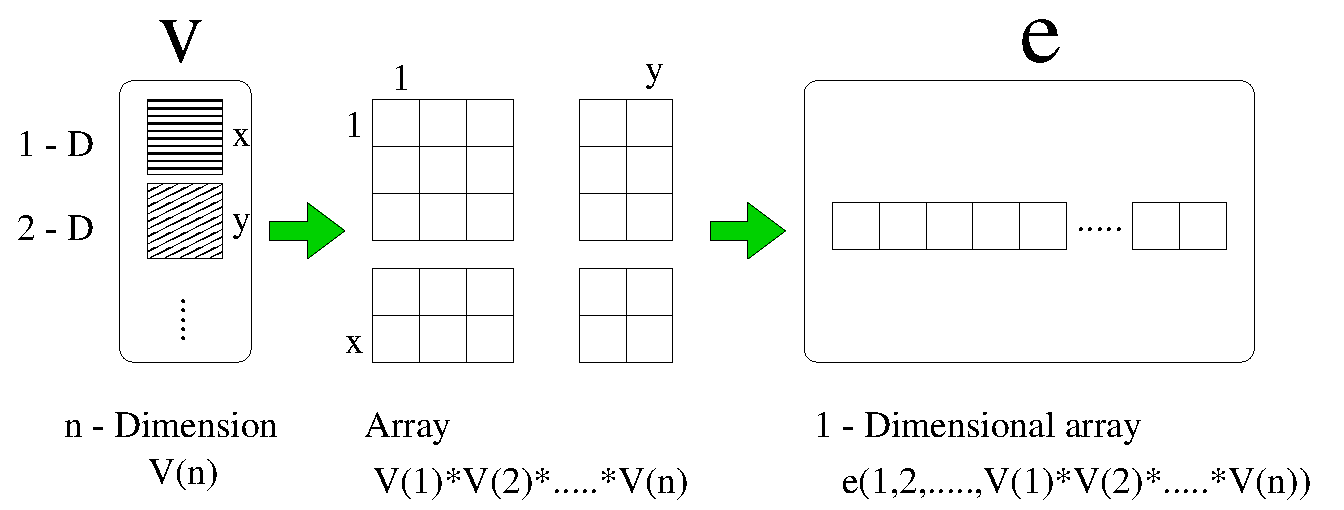
\includegraphics[width=13cm]{array-image.eps}\\
\caption{The organization of arrays in the EALib.}
\label{array}
\end{figure}
\end{center}

\noindent
The vector $d$ contains data about the structure of the array. If $d =
\{ n_1 \}$, this means that the array $e$ is a one dimensional array -
a vector - and the number of elements is $n_1$. If $d = \{ n_1, n_2
\}$, this means that the array $e$ is a two dimensional array - a
matrix - and the number of elements is $n_1 \times n_2$.

\clearpage

\noindent
The vector $e$ contains the actual elements of the array. To explain
this vector, I will use the two dimensional case. The number of
elements are $n_1 \times n_2$. The vector elements from 1 to $n_1$
contain the elements of the first row in the array and the ones from
$n_1+1$ to $2n_1$ contain the elements of the second row, etc.

\vspace*{5mm}

\noindent
In both classes $arraybase$ and $array< Class T>$, the array is
specified by the two vectors $d$ and $e$.

\vspace*{5mm}

\noindent
Caution

\noindent
In C++ programs, the index is from  $0$ to $n-1$ for
$vector[n]$. However, the explanation uses $1$ to $n$. Please bear
this difference in mind !





%************************************************************************
% Class arraybase
%************************************************************************
\clearpage
\chapter{Class {\tt arraybase}}
\index{arraybase}
% 24th, Jan, 2001 Ver.1     Tatsuya Okabe
%                 Ver.2
%                 Ver.3
%                 Ver.4
%                 Ver.5
%
%---------------------------------------------------------------------------%
% Made by Tatsuya Okabe ( HONDA R&D Europe ( Deutschland ) GmbH )           %
% Checked by Bernhard Sendhoff ( HONDA R&D Europe ( Deutschland ) GmbH )    %
%---------------------------------------------------------------------------%
% arraybase

\noindent
In the class {\em arraybase}, functions are defined for treating the
index and changing the structure of an array. Using this class, we can
get information about e.g. the number of dimensions and the number of
elements. Additionally, the structure of the array can be changed.

\vspace*{10mm}

\section{Internal Variables}

\begin{itemize}
\item unsigned* d - The pointer to the dimension vector.
\item unsigned nd - The number of dimensions.
\item unsigned ne - The number of elements
\item bool stat - The flag which signals whether object is a static ref.
\end{itemize}

%********************
\index{*d (Variable)}
\index{nd (Variable)}
\index{ne (Variable)}
\index{stat (Variable)}
%********************

\clearpage

\section{Public Methods}

\subsection{Destructor}

%---------------------------------------------------------------------------%
% 014
\index{$\sim$arraybase!( )}
\setNormalInstance
\printEmptyMethodReturn
{}
{$\sim$arraybase}
{The destructor. Destructs {\em this} object if there is anything to
destruct and it is not a static reference (signalled by the flag
``{\em stat}'').}
{None.}
\setCorrectWidthThree{4pt}
%---------------------------------------------------------------------------%

\vspace*{10mm}

\subsection{Information Retrieval Methos}

%---------------------------------------------------------------------------%
% 001
\index{ndim!( )} 
\setConstInstance
\printEmptyMethodReturnSpecial
{unsigned}
{ndim}
{Returns the number of dimensions, i.e. the length of the index vector.}
{The number of dimensions.}
{None.}
%---------------------------------------------------------------------------%

%---------------------------------------------------------------------------%
% 002
\index{nelem!( )} 
\setConstInstance
\printEmptyMethodReturnSpecial
{unsigned}
{nelem}
{Returns the total number of elements, i.e. the product over all dimensions.}
{The total number of elements.}
{None.}
%---------------------------------------------------------------------------%

\clearpage

\subsection{Structure Changing Methods}

%---------------------------------------------------------------------------%
% 003
\index{samedim!( const arraybase\& v )} 
\setConstInstance
\printMethodWithOneParam
{bool}
{samedim}
{const arraybase\&}
{v}
{The reference array.}
{Checks whether two arrays have the same dimensions independent from
their respective types, returns true if both dimensions are the same.}
{The result of this check.}
{None.}
%---------------------------------------------------------------------------%

%---------------------------------------------------------------------------%
% 004
\index{resize!( unsigned i, bool copy )}
\setNormalInstance
\setCorrectWidthThree{8pt}
\setParamOne{i}{unsigned}{The size of an one-dimensional array.} 
\setParamTwo{copy}{bool}{The flag of copy.}
\printMethodWithParamsSaved
{void}
{None.}
{resize}
{Resizes an array to an one-dimensional array of the size ``{\em i}'', the
flag ``{\em copy}'' signals whether existing elements are copied ( if
possible ).}
{None.}
\setCorrectWidthThree{4pt}
%---------------------------------------------------------------------------%

%---------------------------------------------------------------------------%
% 005
\index{resize!( unsigned i, unsigned j, bool copy )}
\setNormalInstance
\setCorrectWidthThree{8pt}
\setParamOne{i}{unsigned}{The size of an one dimensional array.}
\setParamTwo{j}{unsigned}{The size of the other dimensional array.} 
\setParamThree{copy}{bool}{The flag of copy.}
\printMethodWithParamsSaved
{void}
{None.}
{resize}
{Resizes an array to an two-dimensional array of the size ``{\em i $\times$
j}'', the
flag ``{\em copy}'' signals whether existing elements are copied ( if
possible ).}
{None.}
\setCorrectWidthThree{4pt}
%---------------------------------------------------------------------------%

\clearpage

%---------------------------------------------------------------------------%
% 006
\index{resize!( unsigned i, unsigned j, unsigned k, bool copy )}
\setNormalInstance
\setCorrectWidthThree{8pt}
\setParamOne{i}{unsigned}{The size of an one-dimensional array.}
\setParamTwo{j}{unsigned}{The size of a two-dimensional array.} 
\setParamThree{k}{unsigned}{The size of a three-dimensional array.}
\setParamThree{copy}{bool}{The flag of copy.}
\printMethodWithParamsSaved
{void}
{None.}
{resize}
{Resizes an array to an three-dimensional array of the size ``{\em i $\times$
j $\times$ k}'', the flag ``{\em copy}'' signals whether existing elements
are copied ( if possible ).}
{None.}
\setCorrectWidthThree{4pt}
%---------------------------------------------------------------------------%

%---------------------------------------------------------------------------%
% 007
\index{resize!( const std::vector$<$ unsigned $>$\& i, bool copy )}
\setNormalInstance
\setCorrectWidthThree{8pt}
\setParamOne{i}{const std::vector$<$ unsigned $>$\&}{The vector
setting dimensions.} 
\setParamTwo{copy}{bool}{The flag of copy.}
\printMethodWithParamsSaved
{void}
{None.}
{resize}
{Resizes an array to an array with dimensions defined in vector ``{\em
i}'',
the flag ``{\em copy}'' signals whether existing elements are copied.}
{None.}
\setCorrectWidthThree{4pt}
%---------------------------------------------------------------------------%

%---------------------------------------------------------------------------%
% 009
\index{dim!( unsigned i )} 
\setNormalInstance
\printMethodWithOneParam
{unsigned}
{dim}
{unsigned}
{i}
{The dimension whose value you want to know.}
{Returns the ``{\em i}''th dimension, range check may be performed if not
disabled by the preprocessor directive ``-DNDEBUG''.}
{The ``{\em i}''th dimension.}
{None.}
%---------------------------------------------------------------------------%

\clearpage

%---------------------------------------------------------------------------%
% 010
\index{dimvec!( )} 
\setNormalInstance
\printEmptyMethodReturnSpecial
{unsigned*}
{dimvec}
{Returns the pointer to the dimension vector.}
{The pointer to the dimension vector.}
{Handle with care.}
%---------------------------------------------------------------------------%

%---------------------------------------------------------------------------%
% 011
\index{dimvec!( )} 
\setConstInstance
\printEmptyMethodReturnSpecial
{unsigned*}
{dimvec}
{Returns the pointer to the dimension vector for const objects.}
{The pointer to the dimension vector for const objects.}
{Handle with care.}
%---------------------------------------------------------------------------%

\vspace*{10mm}

\subsection{Generating Methods}

%---------------------------------------------------------------------------%
% 012
\index{clone!( )} 
\setConstInstance
\printEmptyMethodReturnSpecial
{arraybase*}
{clone}
{The pure virtual function which is defined in template class array$<$
T $>$. Returns an identical copy of this object.}
{The pointer.}
{None.}
%---------------------------------------------------------------------------%

%---------------------------------------------------------------------------%
% 013
\index{empty!( )} 
\setConstInstance
\printEmptyMethodReturnSpecial
{arraybase*}
{empty}
{The pure virtual function which is defined in template class array$<$
T $>$. Returns an empty array with the same type as this object.}
{The pointer.}
{None.}
%---------------------------------------------------------------------------%

\clearpage

\section{Private Methods}

\subsection{Constructors}

%---------------------------------------------------------------------------%
% 015
\index{arraybase!( )}
\setNormalInstance
\printEmptyMethodReturnSpecial
{}
{arraybase}
{The default constructor. Initializes the number of dimensions, the
total number of elements and the flag ``{\em stat}'' to false.}
{None.}
{This function should never be used directly.}
\setCorrectWidthThree{4pt}
%---------------------------------------------------------------------------%

%---------------------------------------------------------------------------%
% 016
\index{arraybase!( const arraybase\& v )} 
\setNormalInstance
\printMethodWithOneParam
{}
{arraybase}
{const arraybase\&}
{v}
{The dimension vector.}
{The copy constructor. Only the dimension vector is copied, the data
vector must be copied in the copy constructor of template class
array$<$ T $>$}
{None.}
{This function should never be used directly.}
%---------------------------------------------------------------------------%

\vspace*{10mm}

\subsection{Structure Changing Methods}

%---------------------------------------------------------------------------%
% 017
\index{resize\_i!( unsigned*, unsigned, bool )}
\setNormalInstance
\setCorrectWidthThree{8pt}
\setParamOne{}{unsigned}{} 
\setParamTwo{}{unsigned}{}
\setParamThree{}{bool}{}
\printMethodWithParamsSaved
{void}
{None.}
{resize\_i}
{The pure virtual function. Handles memory allocation of the
respective template type in case of resizing.}
{None.}
\setCorrectWidthThree{4pt}
%---------------------------------------------------------------------------%

\vspace*{10mm}

\subsection{Input and Output Methods}

%---------------------------------------------------------------------------%
% 018
\index{readFrom!( std::istream\& is )} 
\setNormalInstance
\printMethodWithOneParam
{void}
{readFrom}
{std::istream\&}
{is}
{Input stream.}
{Replaces the data of {\em this} with the data read from the input stream
{\em is}.}
{None.}
{None.}
%---------------------------------------------------------------------------%

%---------------------------------------------------------------------------%
% 019
\index{writeTo!( std::ostream\& os )} 
\setConstInstance
\printMethodWithOneParam
{void}
{writeTo}
{std::ostream\&}
{os}
{Output stream.}
{Writes all data of the array {\em this} to the output stream {\em os}.}
{None.}
{None.}
%---------------------------------------------------------------------------%







%************************************************************************
% Class Array< Class T >
%************************************************************************
\clearpage
\chapter{Class {\tt Array$<$ Class T $>$}}
\index{Array$<$ Class T $>$}
% 24th, Jan, 2001 Ver.1     Tatsuya Okabe
%                 Ver.2
%                 Ver.3
%                 Ver.4
%                 Ver.5
%
%---------------------------------------------------------------------------%
% Made by Tatsuya Okabe ( HONDA R&D Europe ( Deutschland ) GmbH )           %
% Checked by Bernhard Sendhoff ( HONDA R&D Europe ( Deutschland ) GmbH )    %
%---------------------------------------------------------------------------%
% Array < Class T >

\noindent
In this class several functions were defined to allow the following
operations on arrays :

\vspace*{10mm}

\begin{enumerate}
\item get (a) value(s) of the array
\item append row(s)
\item append column(s)
\item remove row(s)
\item remove column(s)
\item copy a part of the array
\end{enumerate}

\vspace*{10mm}

\noindent
Additionally, the contents of the array can be rearranged and the
transpose can be calculated.

\vspace*{10mm}

\section{Internal Variables}

\begin{itemize}
\item T* e - The data of array.
\item (arraybase) unsigned* d - The pointer to the dimension vector.
\item (arraybase) unsigned nd - The number of dimensions.
\item (arraybase) unsigned ne - The number of elements
\item (arraybase) bool stat - The flag which signals whether object is a static ref.
\end{itemize}

%********************
\index{*e (Variable)}
\index{*d (Variable)}
\index{nd (Variable)}
\index{ne (Variable)}
\index{stat (Variable)}
%********************

\clearpage

\section{Public Methods}

\subsection{Constructors}

%---------------------------------------------------------------------------%
% 001
\index{array!( )}
\setNormalInstance
\printEmptyMethodReturn
{}
{array}
{The default constructor. Generates empty array.}
{None.}
\setCorrectWidthThree{4pt}
%---------------------------------------------------------------------------%

%---------------------------------------------------------------------------%
% 002
\index{array!( unsigned i )} 
\setNormalInstance
\printMethodWithOneParam
{explicit}
{array}
{unsigned}
{i}
{The size of an one-dimensional array.}
{The copy constructor. Generates new array with one-dimension ``{\em i}''.}
{None.}
{None.}
%---------------------------------------------------------------------------%

%---------------------------------------------------------------------------%
% 003
\index{array!( unsigned i, unsigned j )}
\setNormalInstance
\setCorrectWidthThree{8pt}
\setParamOne{i}{unsigned}{The size of an one-dimensional array.} 
\setParamTwo{j}{unsigned}{The size of a two-dimensional array.}
\printMethodWithParamsSaved
{}
{None.}
{array}
{The copy constructor. Generates new array with two-dimension ``{\em i
$\times$ j}''.}
{None.}
\setCorrectWidthThree{4pt}
%---------------------------------------------------------------------------%

%---------------------------------------------------------------------------%
% 004
\index{array!( unsigned i, unsigned j, unsigned k )}
\setNormalInstance
\setCorrectWidthThree{8pt}
\setParamOne{i}{unsigned}{The size of an one-dimensional array.} 
\setParamTwo{j}{unsigned}{The size of a two-dimensional array.}
\setParamThree{k}{unsigned}{The size of a three-dimensional array.}
\printMethodWithParamsSaved
{}
{None.}
{array}
{The copy constructor. Generates new array with three-dimension ``{\em
i $\times$ j $\times$ k}''.}
{None.}
\setCorrectWidthThree{4pt}
%---------------------------------------------------------------------------%

\clearpage

%---------------------------------------------------------------------------%
% 005
\index{array!( std::vector$<$ T $>$\& v )} 
\setNormalInstance
\printMethodWithOneParam
{}
{array}
{std::vector$<$ T $>$\&}
{v}
{The vector which was set dimensions.}
{The copy constructor. Generates new array from the vector {\em v}.}
{None.}
{None.}
%---------------------------------------------------------------------------%

%---------------------------------------------------------------------------%
% 006
\index{array!( array$<$ T $>$\& v, bool )}
\setNormalInstance
\setCorrectWidthThree{8pt}
\setParamOne{v}{array$<$ T $>$\&}{The array you want copy.} 
\setParamTwo{}{bool}{The dummy value.}
\printMethodWithParamsSaved
{}
{None.}
{array}
{The copy constructor. Generates new array by copying the array ``{\em v}'' and
sets the array ``{\em v}'' as a reference.}
{None.}
\setCorrectWidthThree{4pt}
%---------------------------------------------------------------------------%

%---------------------------------------------------------------------------%
% 007
\index{array!( const array$<$ T $>$\& v)} 
\setNormalInstance
\printMethodWithOneParam
{}
{array}
{const array$<$ T $>$\&}
{v}
{The array you want to copy.}
{The copy construtor. Generates new array by copying the array ``{\em v}'' }
{None.}
{None.}
%---------------------------------------------------------------------------%

\vspace*{10mm}

\subsection{Destructor}

%---------------------------------------------------------------------------%
% 008
\index{$\sim$array!()} 
\setNormalInstance
\printEmptyMethodReturnSpecial
{}
{$\sim$array}
{The distructor. Destroys the current array {\em this}.}
{None.}
{The destructor should not be called directly.}
%---------------------------------------------------------------------------%

\clearpage

\subsection{Operators}

%---------------------------------------------------------------------------%
% 009
\index{operator( )!( )} 
\setNormalInstance
\printEmptyMethodReturn
{T\&}
{operator( )}
{Returns the value {\em e[0]} ( The first value of this array ) if the
number of dimensions is {\em 0} and the number of elements is {\em 1}.}
{The velue of {\em e[0]} ( The first value of this array ).}
%---------------------------------------------------------------------------%

%---------------------------------------------------------------------------%
% 010
\index{operator( )!( )} 
\setConstInstance
\printEmptyMethodReturn
{T\&}
{operator( )}
{Returns the value {\em e[0]} as a constant, if the number of
dimensions is {\em 0} and the number of elements is {\em 1}}
{The value of {\em e[0]} ( The first value of this array ).}
%---------------------------------------------------------------------------%

%---------------------------------------------------------------------------%
% 011
\index{operator( )!( unsigned i )} 
\setNormalInstance
\printMethodWithOneParam
{T\&}
{operator( )}
{unsigned}
{i}
{The number in 1D whose value you want to know.}
{Returns the value {\em e[i]}, if the number of dimensions is {\em 1}
and {\em i} $\le$ the number of elements.}
{The value {\em e[i]}.}
{None.}
%---------------------------------------------------------------------------%

%---------------------------------------------------------------------------%
% 012
\index{operator( )!( unsigned i )} 
\setConstInstance
\printMethodWithOneParam
{T\&}
{operator( )}
{unsigned}
{i}
{The number in 1D whose value you want to know.}
{Returns the value {\em e[i]} as a constant, if the number of
dimensions is {\em 1} and {\em i} $\le$ the number of elements.}
{The value {\em e[i]}.}
{None.}
%---------------------------------------------------------------------------%

\clearpage

%---------------------------------------------------------------------------%
% 013
\index{operator( )!( unsigned i, unsigned j )}
\setNormalInstance
\setCorrectWidthThree{8pt}
\setParamOne{i}{unsigned}{The number in 1D whose you want to know.} 
\setParamTwo{j}{unsigned}{The number in 2D whose you want to know.}
\printMethodWithParamsSaved
{T\&}
{The value of {\em e(i,j)} ( {\em e(d[1]*i+j)} ).}
{operator( )}
{Returns the value {\em e(i,j)}, if the number of dimensions is {\em
2}, {\em i} $\le$ the number of 1-dimensional elements and {\em j} $\le$ the
number of 2-dimensional elements.}
{The value {\em e(i,j)}.}
\setCorrectWidthThree{4pt}
%---------------------------------------------------------------------------%

%---------------------------------------------------------------------------%
% 014
\index{operator( )!( unsigned i, unsigned j )}
\setConstInstance
\setCorrectWidthThree{8pt}
\setParamOne{i}{unsigned}{The number in 1D whose you want to know.} 
\setParamTwo{j}{unsigned}{The number in 2D whose you want to know.}
\printMethodWithParamsSaved
{T\&}
{The value of {\em e(i,j)} ( {\em e(d[1]*i+j)} ).}
{operator( )}
{Returns the value {\em e(i,j)} as a constant, if the number of dimensions is
{\em 2}, {\em i} $\le$ the number of 1-dimensional elements and {\em j} $\le$ the number of 2-dimensional elements.}
{The value {\em e(i,j)}.}
\setCorrectWidthThree{4pt}
%---------------------------------------------------------------------------%

%---------------------------------------------------------------------------%
% 015
\index{operator( )!( unsigned i, unsigned j, unsigned k )}
\setNormalInstance
\setCorrectWidthThree{8pt}
\setParamOne{i}{unsigned}{The number in 1D whose value you want to know.} 
\setParamTwo{j}{unsigned}{The number in 2D whose value you want to konw.}
\setParamThree{k}{unsigned}{The number in 3D whose value you want to know.}
\printMethodWithParamsSaved
{T\&}
{The value of {\em e(i,j,k)} ( {\em e(d[2]*d[1]*i+d[2]*j+k )} ).}
{operator( )}
{Returns the value {\em e(i,j,k)}, if the number of dimensions is {\em
3}, {\em i} $\le$
the number of 1-dimensional elements, {\em j} $\le$ the
number of 2-dimensional elements and {\em k} $\le$ the number of
3-dimensional elements.}
{The value {\em e(i,j,k)}.}
\setCorrectWidthThree{4pt}
%---------------------------------------------------------------------------%

\clearpage

%---------------------------------------------------------------------------%
% 016
\index{operator( )!( unsigned i, unsigned j, unsigned k )}
\setConstInstance
\setCorrectWidthThree{8pt}
\setParamOne{i}{unsigned}{The number in 1D whose value you want to know.} 
\setParamTwo{j}{unsigned}{The number in 2D whose value you want to know.}
\setParamThree{k}{unsigned}{The number in 3D whose value you want to know.}
\printMethodWithParamsSaved
{T\&}
{The value of {\em e(i,j,k)} ( {\em e(d[2]*d[1]*i+d[2]*j+k )} ).}
{operator( )}
{Returns the value {\em e(i,j,k)} as a constant, if the number of
dimensions is {\em 3}, {\em i} $\le$
the number of 1-dimensional elements, {\em j} $\le$ the
number of 2-dimensional elements and {\em k} $\le$ the number of
3-dimensional elements.}
{The value {\em e(i,j,k)}.}
\setCorrectWidthThree{4pt}
%---------------------------------------------------------------------------%

%---------------------------------------------------------------------------%
% 017
\index{operator( )!( const std::vector$<$ unsigned $>$\& i )} 
\setNormalInstance
\printMethodWithOneParam
{T\&}
{operator( )}
{const std::vector$<$ unsigned $>$\&}
{i}
{The vector which indicates the position of the array, e.g. {\em (i)} : 1D,
{\em (i,j)} : 2D or {\em (i,j,k)} : 3D. Instead of each integer, the
vector ``{\em i}'' is used.}
{Returns the value {\em e(m)}.}
{The value {\em e(i)}.}
{None.}
%---------------------------------------------------------------------------%

%---------------------------------------------------------------------------%
% 018
\index{operator( )!( const std::vector$<$ unsigned $>$\& i )} 
\setConstInstance
\printMethodWithOneParam
{T\&}
{operator( )}
{const std::vector$<$ unsigned $>$\&}
{i}
{The vector which indicates the position of the array, e.g. {\em (i)} : 1D,
{\em (i,j)} : 2D or {\em (i,j,k)} : 3D. Instead of each integer, the
vector ``{\em i}'' is used.}
{Returns the value {\em e(m)} as a constant.}
{The value {\em e(m)}.}
{None.}
%---------------------------------------------------------------------------%

%---------------------------------------------------------------------------%
% 019
%\index{} 
%\setNormalInstance
%\printMethodWithOneParam
%{array\_reference$<$ T $>$}
%{operator[ ]}
%{unsigned}
%{i}
%{}
%{}
%{}
%{The corresponding codes are commented out.}
%---------------------------------------------------------------------------%

%---------------------------------------------------------------------------%
% 020
%\index{} 
%\setConstInstance
%\printMethodWithOneParam
%{array\_reference$<$ T $>$}
%{operator[ ]}
%{unsigned}
%{i}
%{}
%{}
%{}
%{The corresponding codes are commented out.}
%---------------------------------------------------------------------------%

%---------------------------------------------------------------------------%
% 021
\index{operator =!( const T\& v )} 
\setNormalInstance
\printMethodWithOneParam
{array$<$ T $>$\&}
{operator =}
{const T\&}
{v}
{The normal array in \cpp.}
{Changes the ``{\em v}'' into the array in this class {\em array}.}
{The array ``{\em this}''.}
{None.}
%---------------------------------------------------------------------------%

\clearpage

%---------------------------------------------------------------------------%
% 022
\index{operator =!( const std::vector$<$ T $>$\& v} 
\setNormalInstance
\printMethodWithOneParam
{array$<$ T $>$\&}
{operator=}
{const std::vector$<$ T $>$\&}
{v}
{The vector.}
{Changes the ``{\em v}'' into the array in this class {\em array}.}
{The array ``{\em this}''.}
{None.}
%---------------------------------------------------------------------------%

%---------------------------------------------------------------------------%
% 023
\index{operator =!( const array$<$ T $>$\& v )} 
\setNormalInstance
\printMethodWithOneParam
{array$<$ T $>$\&}
{operator=}
{const array$<$ T $>$\&}
{v}
{The array ``{\em v}''.}
{Handles the special case of assigning an empty array in order to
avoid uninitialized memory read (purify).}
{The array from ``{\em this}''.}
{None.}
%---------------------------------------------------------------------------%

\clearpage

\subsection{Methods of getting the data in the array.}

%---------------------------------------------------------------------------%
% 024
\index{elem!( unsigned i )} 
\setNormalInstance
\printMethodWithOneParam
{T\&}
{elem}
{unsigned}
{i}
{The number of data you want to get.}
{Returns the value of ``{\em i}''th data in the array.}
{The value of ``{\em i}''th data in the array ``{\em e[i]}''.}
{None.}
%---------------------------------------------------------------------------%

%---------------------------------------------------------------------------%
% 025
\index{elem!( unsigned i )} 
\setConstInstance
\printMethodWithOneParam
{T\&}
{elem}
{unsigned}
{i}
{The number of data you want to get.}
{Returns the value of ``{\em i}''th data in the array as a constant.}
{The value of ``{\em i}''th data in the array ``{\em e[i]}''.}
{None.}
%---------------------------------------------------------------------------%

%---------------------------------------------------------------------------%
% 026
\index{elemvec!( )} 
\setNormalInstance
\printEmptyMethodReturn
{T*}
{elemvec}
{Returns the vector ``{\em e}''.}
{The vector ``{\em e}''.}
%---------------------------------------------------------------------------%

%---------------------------------------------------------------------------%
% 026a
\index{elemvec!( )} 
\setConstInstance
\printEmptyMethodReturn
{T*}
{elemvec}
{Returns the vector ``{\em e}'' as a constant.}
{The vector ``{\em e}''.}
%---------------------------------------------------------------------------%

%---------------------------------------------------------------------------%
% 067
\index{dimarr!( )} 
\setConstInstance
\printEmptyMethodReturn
{array$<$ unsigned $>$}
{dimarr}
{Returns the dimension array ( vector ) ``{\em d}''.}
{The dimension array ``{\em d}''.}
%---------------------------------------------------------------------------%

\clearpage

\subsection{Structure Changing Methods}

\vspace*{5mm}

\noindent
Append.

%---------------------------------------------------------------------------%
% 027
\index{append\_elem!( const T\& w )} 
\setNormalInstance
\printMethodWithOneParam
{array$<$ T $>$\&}
{append\_elem}
{const T\&}
{w}
{The data you want to append in this array.}
{Appends the data.}
{The array ``{\em this}''.}
{This function needs the empty or 1-Dimensional array.}
%---------------------------------------------------------------------------%

%---------------------------------------------------------------------------%
% 028
\index{append\_elems!( const array$<$ T $>$\& w )} 
\setNormalInstance
\printMethodWithOneParam
{array$<$ T $>$\&}
{append\_elems}
{const array$<$ T $>$\&}
{w}
{The array you want to append in this array.}
{Appends the array ( 1-Dimension ).}
{The array ``{\em this}''.}
{This functioin needs the empty or 1-Dimensional array.}
%---------------------------------------------------------------------------%

%---------------------------------------------------------------------------%
% 029
\index{append\_rows!( const array$<$ T $>$\& y} 
\setNormalInstance
\printMethodWithOneParam
{array$<$ T $>$\&}
{append\_rows}
{const array$<$ T $>$\&}
{y}
{The array you want to append after the last row of this array.}
{Appends the array ``{\em y}'' after the last row.}
{The array {\em this}.}
{This function needs the empty array or the same dimensional array or
-1 dimensional array of {\em y}.}
%---------------------------------------------------------------------------%

%---------------------------------------------------------------------------%
% 040
\index{append\_cols!( const array$<$ T $>$\& y )} 
\setConstInstance
\printMethodWithOneParam
{array$<$ T $>$\&}
{append\_cols}
{const array$<$ T $>$\&}
{y}
{The array you want to append after the last column of this array.}
{Appends the array ``{\em y}'' after the last column.}
{The array ( result ).}
{This function needs that this array is empty or the dimension of this
array is equal to ``{\em y}''.}
%---------------------------------------------------------------------------%

\clearpage

\noindent
Remove.

%---------------------------------------------------------------------------%
% 030
\index{remove\_row!( unsigned i )} 
\setNormalInstance
\printMethodWithOneParam
{array$<$ T $>$\&}
{remove\_row}
{unsigned}
{i}
{The number of row you want to remove. The number starts from {\em 0}.}
{Removes one row from the array.}
{The array ``{\em this}''.}
{This function needs that the dimension of this array is larger than
{\em 0} and ``{\em i}'' is less than or equal to ``{\em d[0]}''.}
%---------------------------------------------------------------------------%

%---------------------------------------------------------------------------%
% 031
\index{remove\_col!( unsigned k )} 
\setConstInstance
\printMethodWithOneParam
{array$<$ T $>$\&}
{remove\_col}
{unsigned}
{k}
{The number of column you want to remove. The number starts from {\em 0}.}
{Removes one column form the array.}
{The array ( result ).}
{This function needs that the dimension of this array is larger than
{\em 0}
and ``{\em i}'' is less than ``{\em dim( ndim( )-1 )}''.}
%---------------------------------------------------------------------------%

%---------------------------------------------------------------------------%
% 032
\index{remove\_cols!( const array$<$ unsigned $>$ idx )} 
\setConstInstance
\printMethodWithOneParam
{array$<$ T $>$}
{remove\_cols}
{const array$<$ unsigned $>$}
{idx}
{The array which has the numbers of columns you want to remove.}
{Removes columns from the array.}
{The array ( result ).}
{None.}
%---------------------------------------------------------------------------%

%---------------------------------------------------------------------------%
% 033
\index{remove\_cols!( unsigned i, unsigned j )}
\setConstInstance
\setCorrectWidthThree{8pt}
\setParamOne{i}{unsigned}{The number of column you want to remove.} 
\setParamTwo{j}{unsigned}{The number of column you want to remove.}
\printMethodWithParamsSaved
{array$<$ T $>$}
{The array ( result ).}
{remove\_cols}
{Removes two columns ``{\em i}'' and ``{\em j}'' from the array.}
{None.}
\setCorrectWidthThree{4pt}
%---------------------------------------------------------------------------%

\clearpage

%---------------------------------------------------------------------------%
% 034
\index{remove\_cols!( unsigned i, unsigned j, unsigned k)}
\setConstInstance
\setCorrectWidthThree{8pt}
\setParamOne{i}{unsigned}{The number of column you want to remove.} 
\setParamTwo{j}{unsigned}{The number of column you want to remove.}
\setParamThree{k}{unsigned}{The number of column you want to remove.}
\printMethodWithParamsSaved
{array$<$ T $>$}
{The array ( result ).}
{remove\_cols}
{Removes three columns ``{\em i}'', ``{\em j}'' and ``{\em k}'' from the array.}
{None.}
\setCorrectWidthThree{4pt}
%---------------------------------------------------------------------------%

\vspace*{-3mm}

%---------------------------------------------------------------------------%
% 035
\index{remove\_cols!( unsigned i, unsigned j, unsigned k, unsinged l )}
\setConstInstance
\setCorrectWidthThree{8pt}
\setParamOne{i}{unsigned}{The number of column you want to remove.} 
\setParamTwo{j}{unsigned}{The number of column you want to remove.}
\setParamThree{k}{unsigned}{The number of column you want to remove.}
\setParamFour{l}{unsigned}{The number of column you want to remove.}
\printMethodWithParamsSaved
{array$<$ T $>$}
{The array ( result ).}
{remove\_cols}
{Removes four columns ``{\em i}'', ``{\em j}'', ``{\em k}'' and ``{\em
l}'' from the array.}
{None.}
\setCorrectWidthThree{4pt}
%---------------------------------------------------------------------------%

\vspace*{-3mm}

%---------------------------------------------------------------------------%
% 036
\index{remove\_cols!( unsigned i, unsigned j, unsigned k, unsinged l,
unsigned m )}
\setConstInstance
\setCorrectWidthThree{8pt}
\setParamOne{i}{unsigned}{The number of column you want to remove.} 
\setParamTwo{j}{unsigned}{The number of column you want to remove.}
\setParamThree{k}{unsigned}{The number of column you want to remove.}
\setParamFour{l}{unsigned}{The number of column you want to remove.}
\setParamFive{m}{unsigned}{The number of column you want to remove.}
\printMethodWithParamsSaved
{array$<$ T $>$}
{The array ( result ).}
{remove\_cols}
{Removes five columns ``{\em i}'', ``{\em j}'', ``{\em k}'' ``{\em
l}'' and ``{\em m}'' from the array.}
{None.}
\setCorrectWidthThree{4pt}
%---------------------------------------------------------------------------%

\clearpage

%---------------------------------------------------------------------------%
% 037
\index{remove\_cols!( unsigned i, unsigned j, unsigned k, unsinged l,
unsigned m, unsigned n )}
\setConstInstance
\setCorrectWidthThree{8pt}
\setParamOne{i}{unsigned}{The number of column you want to remove.} 
\setParamTwo{j}{unsigned}{The number of column you want to remove.}
\setParamThree{k}{unsigned}{The number of column you want to remove.}
\setParamFour{l}{unsigned}{The number of column you want to remove.}
\setParamFive{m}{unsigned}{The number of column you want to remove.}
\setParamSix{n}{unsigned}{The number of column you want to remove.}
\printMethodWithParamsSaved
{array$<$ T $>$}
{The array ( result ).}
{remove\_cols}
{Removes six columns ``{\em i}'', ``{\em j}'', ``{\em k}'' ``{\em
l}'', ``{\em m}''  and ``{\em n}'' from the array.}
{None.}
\setCorrectWidthThree{4pt}
%---------------------------------------------------------------------------%

%---------------------------------------------------------------------------%
% 038
\index{remove\_cols!( unsigned i, unsigned j, unsigned k, unsinged l,
unsigned m, unsigned n, unsigned o )}
\setConstInstance
\setCorrectWidthThree{8pt}
\setParamOne{i}{unsigned}{The number of column you want to remove.} 
\setParamTwo{j}{unsigned}{The number of column you want to remove.}
\setParamThree{k}{unsigned}{The number of column you want to remove.}
\setParamFour{l}{unsigned}{The number of column you want to remove.}
\setParamFive{m}{unsigned}{The number of column you want to remove.}
\setParamSix{n}{unsigned}{The number of column you want to remove.}
\setParamSeven{o}{unsigned}{The number of column you want to remove.}
\printMethodWithParamsSaved
{array$<$ T $>$}
{The array ( result ).}
{remove\_cols}
{Removes seven columns ``{\em i}'', ``{\em j}'', ``{\em k}'' ``{\em l}'', ``{\em m}'', ``{\em n}''  and ``{\em o}'' from the array.}
{None.}
\setCorrectWidthThree{4pt}
%---------------------------------------------------------------------------%

\clearpage

%---------------------------------------------------------------------------%
% 039
\index{remove\_cols!( unsigned i, unsigned j, unsigned k, unsinged l,
unsigned m, unsigned n, unsigned o, unsigned p )}
\setConstInstance
\setCorrectWidthThree{8pt}
\setParamOne{i}{unsigned}{The number of column you want to remove.} 
\setParamTwo{j}{unsigned}{The number of column you want to remove.}
\setParamThree{k}{unsigned}{The number of column you want to remove.}
\setParamFour{l}{unsigned}{The number of column you want to remove.}
\setParamFive{m}{unsigned}{The number of column you want to remove.}
\setParamSix{n}{unsigned}{The number of column you want to remove.}
\setParamSeven{o}{unsigned}{The number of column you want to remove.}
\setParamEight{p}{unsigned}{The number of column you want to remove.}
\printMethodWithParamsSaved
{array$<$ T $>$}
{The array ( result ).}
{remove\_cols}
{Removes eight columns ``{\em i}'', ``{\em j}'', ``{\em k}'' ``{\em l}'', ``{\em m}'', ``{\em n}'', ``{\em o}''  and ``{\em p}'' from the array.}
{None.}
\setCorrectWidthThree{4pt}
%---------------------------------------------------------------------------%

\clearpage
\subsection{Methods of picking up parts of the array.}

%---------------------------------------------------------------------------%
% 041
\index{subarr!( unsigned from, unsigned to )}
\setConstInstance
\setCorrectWidthThree{8pt}
\setParamOne{from}{unsigned}{The begining of data you want to pick up.} 
\setParamTwo{to}{unsigned}{The end of data you want to pick up.}
\printMethodWithParamsSaved
{array$<$ T $>$}
{The array ( result ).}
{subarr}
{Picks up parts of the array from ``{\em from}'' to ``{\em to}''.}
{None.}
\setCorrectWidthThree{4pt}
%---------------------------------------------------------------------------%

%---------------------------------------------------------------------------%
% 042
\index{pos2idx!( unsigned p )} 
\setConstInstance
\printMethodWithOneParam
{array$<$ unsigned $>$\&}
{pos2idx}
{unsigned}
{p}
{The number you want to calculate {\em (i)} or {\em (i,j)} or {\em (i,j,k)}. (
The number starts from {\em 0} and ends to ``{\em ne-1}'' ).}
{Calculates the vector which indicates the position of the array like
{\em (i,j,k)} from the consequential order.}
{The vector which indicate the position of the array.}
{None.}
%---------------------------------------------------------------------------%

%---------------------------------------------------------------------------%
% 043
%\index{} 
%\setNormalInstance
%\printMethodWithOneParam
%{array$<$ unsigned $>$\&}
%{whereis}
%{const T\&}
%{y}
%{}
%{}
%{}
%{This function was commented out.}
%---------------------------------------------------------------------------%

%---------------------------------------------------------------------------%
% 044
\index{row!( unsigned i )} 
\setConstInstance
\printMethodWithOneParam
{array$<$ T $>$}
{row}
{unsigned}
{i}
{The number of row you want to pick up.}
{Picks up one row from the array.}
{The array ( result ) {\em (*this)[i]}.}
{None.}
%---------------------------------------------------------------------------%

%---------------------------------------------------------------------------%
% 045
\index{rows!( const array$<$ unsigned $>$\& idx )} 
\setConstInstance
\printMethodWithOneParam
{array$<$ T $>$}
{rows}
{const array$<$ unsigned $>$\&}
{idx}
{The vector which includes numbers of rows you want to pick up.}
{Picks up rows from the array.}
{The array ( result ).}
{None.}
%---------------------------------------------------------------------------%

\clearpage

%---------------------------------------------------------------------------%
% 046
\index{rows!( unsigned i )} 
\setConstInstance
\printMethodWithOneParam
{array$<$ T $>$}
{rows}
{unsigned}
{i}
{The number of row you want to pick up.}
{Picks up one row ``{\em i}'' from the array.}
{The array ( result ).}
{None.}
%---------------------------------------------------------------------------%

%---------------------------------------------------------------------------%
% 047
\index{rows!( unsigned i, unsigned j )}
\setConstInstance
\setCorrectWidthThree{8pt}
\setParamOne{i}{unsigned}{The number of row you want to pick up.} 
\setParamTwo{j}{unsigned}{The number of row you want to pick up.}
\printMethodWithParamsSaved
{array$<$ T $>$}
{The array ( result ).}
{rows}
{Picks up two rows ``{\em i}'' and ``{\em j}'' from the array.}
{None.}
\setCorrectWidthThree{4pt}
%---------------------------------------------------------------------------%

%---------------------------------------------------------------------------%
% 048
\index{rows!( unsigned i, unsigned j, unsigned k )}
\setConstInstance
\setCorrectWidthThree{8pt}
\setParamOne{i}{unsigned}{The number of row you want to pick up.} 
\setParamTwo{j}{unsigned}{The number of row you want to pick up.}
\setParamThree{k}{unsigned}{The number of row you want to pick up.}
\printMethodWithParamsSaved
{array$<$ T $>$}
{The array ( result ).}
{rows}
{Picks up three rows ``{\em i}'', ``{\em j}'' and ``{\em k}'' from the array.}
{None.}
\setCorrectWidthThree{4pt}
%---------------------------------------------------------------------------%

\clearpage

%---------------------------------------------------------------------------%
% 049
\index{rows!( unsigned i, unsigned j, unsigned k, unsigned l )}
\setConstInstance
\setCorrectWidthThree{8pt}
\setParamOne{i}{unsigned}{The number of row you want to pick up.} 
\setParamTwo{j}{unsigned}{The number of row you want to pick up.}
\setParamThree{k}{unsigned}{The number of row you want to pick up.}
\setParamFour{l}{unsigned}{The number of row you want to pick up.}
\printMethodWithParamsSaved
{array$<$ T $>$}
{The array ( result ).}
{rows}
{Picks up four rows ``{\em i}'', ``{\em j}'', ``{\em k}'' and ``{\em l}'' from the array.}
{None.}
\setCorrectWidthThree{4pt}
%---------------------------------------------------------------------------%

%---------------------------------------------------------------------------%
% 050
\index{rows!( unsigned i, unsigned j, unsigned k, unsigned l,
unsigned m )}
\setConstInstance
\setCorrectWidthThree{8pt}
\setParamOne{i}{unsigned}{The number of row you want to pick up.} 
\setParamTwo{j}{unsigned}{The number of row you want to pick up.}
\setParamThree{k}{unsigned}{The number of row you want to pick up.}
\setParamFour{l}{unsigned}{The number of row you want to pick up.}
\setParamFive{m}{unsigned}{The number of row you want to pick up.}
\printMethodWithParamsSaved
{array$<$ T $>$}
{The array ( result ).}
{rows}
{Picks up five rows ``{\em i}'', ``{\em j}'', ``{\em k}'', ``{\em l}'' and ``{\em m}'' from the array.}
{None.}
\setCorrectWidthThree{4pt}
%---------------------------------------------------------------------------%

\clearpage

%---------------------------------------------------------------------------%
% 051
\index{rows!( unsigned i, unsigned j, unsigned k, unsigned l,
unsigned m, unsigned n )}
\setConstInstance
\setCorrectWidthThree{8pt}
\setParamOne{i}{unsigned}{The number of row you want to pick up.} 
\setParamTwo{j}{unsigned}{The number of row you want to pick up.}
\setParamThree{k}{unsigned}{The number of row you want to pick up.}
\setParamFour{l}{unsigned}{The number of row you want to pick up.}
\setParamFive{m}{unsigned}{The number of row you want to pick up.}
\setParamSix{n}{unsigned}{The number of row you want to pick up.}
\printMethodWithParamsSaved
{array$<$ T $>$}
{The array ( result ).}
{rows}
{Picks up six rows ``{\em i}'', ``{\em j}'', ``{\em k}'', ``{\em l}'', ``{\em m}'' and ``{\em n}'' from the array.}
{None.}
\setCorrectWidthThree{4pt}
%---------------------------------------------------------------------------%

%---------------------------------------------------------------------------%
% 052
\index{rows!( unsigned i, unsigned j, unsigned k, unsigned l,
unsigned m, unsigned n, unsigned o )}
\setConstInstance
\setCorrectWidthThree{8pt}
\setParamOne{i}{unsigned}{The number of row you want to pick up.} 
\setParamTwo{j}{unsigned}{The number of row you want to pick up.}
\setParamThree{k}{unsigned}{The number of row you want to pick up.}
\setParamFour{l}{unsigned}{The number of row you want to pick up.}
\setParamFive{m}{unsigned}{The number of row you want to pick up.}
\setParamSix{n}{unsigned}{The number of row you want to pick up.}
\setParamSeven{o}{unsigned}{The number of row you want to pick up.}
\printMethodWithParamsSaved
{array$<$ T $>$}
{The array ( result ).}
{rows}
{Picks up seven rows ``{\em i}'', ``{\em j}'', ``{\em k}'', ``{\em l}'', ``{\em m}'', ``{\em n}'' and ``{\em o}'' from the array.}
{None.}
\setCorrectWidthThree{4pt}
%---------------------------------------------------------------------------%

\clearpage

%---------------------------------------------------------------------------%
% 053
\index{rows!( unsigned i, unsigned j, unsigned k, unsigned l,
unsigned m, unsigned n, unsigned o, unsigned p )}
\setConstInstance
\setCorrectWidthThree{8pt}
\setParamOne{i}{unsigned}{The number of row you want to pick up.} 
\setParamTwo{j}{unsigned}{The number of row you want to pick up.}
\setParamThree{k}{unsigned}{The number of row you want to pick up.}
\setParamFour{l}{unsigned}{The number of row you want to pick up.}
\setParamFive{m}{unsigned}{The number of row you want to pick up.}
\setParamSix{n}{unsigned}{The number of row you want to pick up.}
\setParamSeven{o}{unsigned}{The number of row you want to pick up.}
\setParamEight{p}{unsigned}{The number of row you want to pick up.}
\printMethodWithParamsSaved
{array$<$ T $>$}
{The array ( result ).}
{rows}
{Picks up eight rows ``{\em i}'', ``{\em j}'', ``{\em k}'', ``{\em l}'', ``{\em m}'', ``{\em n}'', ``{\em o}'' and ``{\em p}'' from the array.}
{None.}
\setCorrectWidthThree{4pt}
%---------------------------------------------------------------------------%

%---------------------------------------------------------------------------%
% 054
\index{col!( unsigned i )} 
\setConstInstance
\printMethodWithOneParam
{array$<$ T $>$}
{col}
{unsigned}
{i}
{The number of column you want to pick up.}
{Picks up one column ``{\em i}'' from the array.}
{The array ( result ).}
{None.}
%---------------------------------------------------------------------------%

%---------------------------------------------------------------------------%
% 055
\index{cols!( const array$<$ unsigned $>$\& idx )} 
\setConstInstance
\printMethodWithOneParam
{array$<$ T $>$}
{cols}
{const array$<$ unsigned $>$\&}
{idx}
{The vector which includes numbers of columns you want to pick up.}
{Picks up columns form the array.}
{The array ( result ).}
{None.}
%---------------------------------------------------------------------------%

\clearpage

%---------------------------------------------------------------------------%
% 056
\index{cols!( unsigned i )} 
\setConstInstance
\printMethodWithOneParam
{array$<$ T $>$}
{cols}
{unsigned}
{i}
{The number of column you want to pick up.}
{Picks up one column ``{\em i}'' form the array.}
{The array ( result ).}
{This function is the same ``{\em col( unsinged i )}''.}
%---------------------------------------------------------------------------%

%---------------------------------------------------------------------------%
% 057
\index{cols!( unsigned i, unsigned j )}
\setConstInstance
\setCorrectWidthThree{8pt}
\setParamOne{i}{unsigned}{The number of column you want to pick up.} 
\setParamTwo{j}{unsigned}{The number of column you want to pick up.}
\printMethodWithParamsSaved
{array$<$ T $>$}
{The array ( result ).}
{cols}
{Picks up two columns ``{\em i}'' and ``{\em j}'' from the array.}
{None.}
\setCorrectWidthThree{4pt}
%---------------------------------------------------------------------------%

%---------------------------------------------------------------------------%
% 058
\index{cols!( unsigned i, unsigned j, unsigned k )}
\setConstInstance
\setCorrectWidthThree{8pt}
\setParamOne{i}{unsigned}{The number of column you want to pick up.} 
\setParamTwo{j}{unsigned}{The number of column you want to pick up.}
\setParamThree{k}{unsigned}{The number of column you want to pick up.}
\printMethodWithParamsSaved
{array$<$ T $>$}
{The array ( result ).}
{cols}
{Picks up three columns ``{\em i}'', ``{\em j}'' and ``{\em k}'' from the array.}
{None.}
\setCorrectWidthThree{4pt}
%---------------------------------------------------------------------------%

\clearpage

%---------------------------------------------------------------------------%
% 059
\index{cols!( unsigned i, unsigned j, unsigned k, unsigned l )}
\setConstInstance
\setCorrectWidthThree{8pt}
\setParamOne{i}{unsigned}{The number of column you want to pick up.} 
\setParamTwo{j}{unsigned}{The number of column you want to pick up.}
\setParamThree{k}{unsigned}{The number of column you want to pick up.}
\setParamFour{l}{unsigned}{The number of column you want to pick up.}
\printMethodWithParamsSaved
{array$<$ T $>$}
{The array ( result ).}
{cols}
{Picks up four columns ``{\em i}'', ``{\em j}'', ``{\em k}'' and ``{\em l}'' from the array.}
{None.}
\setCorrectWidthThree{4pt}
%---------------------------------------------------------------------------%

%---------------------------------------------------------------------------%
% 060
\index{cols!( unsigned i, unsigned j, unsigned k, unsigned l, unsigned
m )}
\setConstInstance
\setCorrectWidthThree{8pt}
\setParamOne{i}{unsigned}{The number of column you want to pick up.} 
\setParamTwo{j}{unsigned}{The number of column you want to pick up.}
\setParamThree{k}{unsigned}{The number of column you want to pick up.}
\setParamFour{l}{unsigned}{The number of column you want to pick up.}
\setParamFive{m}{unsigned}{The number of column you want to pick up.}
\printMethodWithParamsSaved
{array$<$ T $>$}
{The array ( result ).}
{cols}
{Picks up five columns ``{\em i}'', ``{\em j}'', ``{\em k}'', ``{\em l}'' and ``{\em m}'' from the array.}
{None.}
\setCorrectWidthThree{4pt}
%---------------------------------------------------------------------------%

\clearpage

%---------------------------------------------------------------------------%
% 061
\index{cols!( unsigned i, unsigned j, unsigned k, unsigned l, unsigned
m, unsigned n )}
\setConstInstance
\setCorrectWidthThree{8pt}
\setParamOne{i}{unsigned}{The number of column you want to pick up.} 
\setParamTwo{j}{unsigned}{The number of column you want to pick up.}
\setParamThree{k}{unsigned}{The number of column you want to pick up.}
\setParamFour{l}{unsigned}{The number of column you want to pick up.}
\setParamFive{m}{unsigned}{The number of column you want to pick up.}
\setParamSix{n}{unsigned}{The number of column you want to pick up.}
\printMethodWithParamsSaved
{array$<$ T $>$}
{The array ( result ).}
{cols}
{Picks up six columns ``{\em i}'', ``{\em j}'', ``{\em k}'', ``{\em l}'', ``{\em m}'' and ``{\em n}'' from the array.}
{None.}
\setCorrectWidthThree{4pt}
%---------------------------------------------------------------------------%

%---------------------------------------------------------------------------%
% 062
\index{cols!( unsigned i, unsigned j, unsigned k, unsigned l, unsigned
m, unsigned n, unsigned o )}
\setConstInstance
\setCorrectWidthThree{8pt}
\setParamOne{i}{unsigned}{The number of column you want to pick up.} 
\setParamTwo{j}{unsigned}{The number of column you want to pick up.}
\setParamThree{k}{unsigned}{The number of column you want to pick up.}
\setParamFour{l}{unsigned}{The number of column you want to pick up.}
\setParamFive{m}{unsigned}{The number of column you want to pick up.}
\setParamSix{n}{unsigned}{The number of column you want to pick up.}
\setParamSeven{o}{unsigned}{The number of column you want to pick up.}
\printMethodWithParamsSaved
{array$<$ T $>$}
{The array ( result ).}
{cols}
{Picks up seven columns ``{\em i}'', ``{\em j}'', ``{\em k}'', ``{\em l}'', ``{\em m}'', ``{\em n}'' and ``{\em o}'' from the array.}
{None.}
\setCorrectWidthThree{4pt}
%---------------------------------------------------------------------------%

\clearpage

%---------------------------------------------------------------------------%
% 063
\index{cols!( unsigned i, unsigned j, unsigned k, unsigned l, unsigned
m, unsigned n, unsigned o, unsigned p )}
\setConstInstance
\setCorrectWidthThree{8pt}
\setParamOne{i}{unsigned}{The number of column you want to pick up.} 
\setParamTwo{j}{unsigned}{The number of column you want to pick up.}
\setParamThree{k}{unsigned}{The number of column you want to pick up.}
\setParamFour{l}{unsigned}{The number of column you want to pick up.}
\setParamFive{m}{unsigned}{The number of column you want to pick up.}
\setParamSix{n}{unsigned}{The number of column you want to pick up.}
\setParamSeven{o}{unsigned}{The number of column you want to pick up.}
\setParamEight{p}{unsigned}{The number of column you want to pick up.}
\printMethodWithParamsSaved
{array$<$ T $>$}
{The array ( result ).}
{cols}
{Picks up seven columns ``{\em i}'', ``{\em j}'', ``{\em k}'', ``{\em l}'', ``{\em m}'', ``{\em n}'', ``{\em o}'' and ``{\em p}'' from the array.}
{None.}
\setCorrectWidthThree{4pt}
%---------------------------------------------------------------------------%

\clearpage

\subsection{Methods for arranging the array.}

%---------------------------------------------------------------------------%
% 064
\index{transpose!( )} 
\setNormalInstance
\printEmptyMethodReturn
{array$<$ T $>$\&}
{transpose}
{Calculates the transopose array.}
{The array ``{\em this}''.}
%---------------------------------------------------------------------------%

%---------------------------------------------------------------------------%
% 065
\index{rotate\_rows!( int n )} 
\setConstInstance
\printMethodWithOneParam
{array$<$ T $>$}
{rotate\_rows}
{int}
{n}
{The number of rows you want to put first.}
{Changes the order of rows.}
{The array ( result ).}
{None.}
%---------------------------------------------------------------------------%

\begin{center}
\begin{figure}[h]
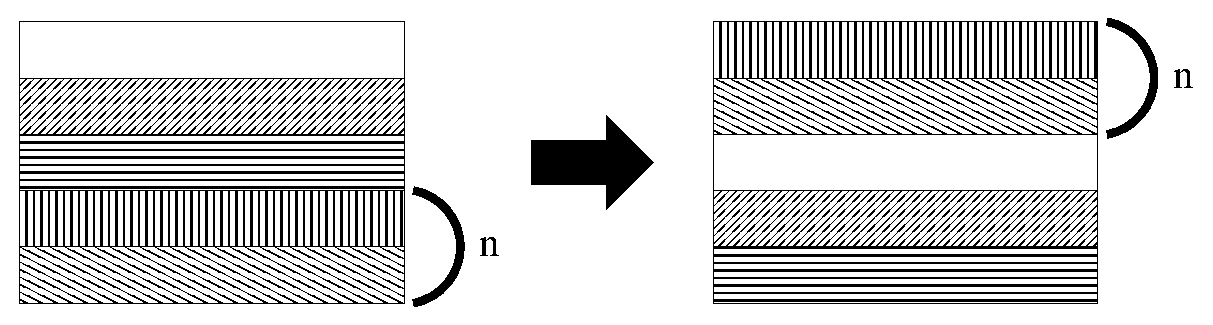
\includegraphics[width=12cm]{rotate-rows.eps}\\
\caption{Rotate-rows function.}
\end{figure}
\end{center}

\vspace*{-5mm}

%---------------------------------------------------------------------------%
% 066
\index{rotate\_cols!( int n )} 
\setNormalInstance
\printMethodWithOneParam
{array$<$ T $>$}
{rotate\_cols}
{int}
{n}
{The number of columns you want to put first ( See above ).}
{Changes the order of rows.}
{The array ( result ).}
{None.}
%---------------------------------------------------------------------------%

\clearpage

\subsection{Generating Methods}

%---------------------------------------------------------------------------%
% 068
\index{clone!( )} 
\setConstInstance
\printEmptyMethodReturn
{arraybase*}
{clone}
{Returns a copy of the current array.}
{A copy of the current array.}
%---------------------------------------------------------------------------%

%---------------------------------------------------------------------------%
% 069
\index{empty!( )} 
\setConstInstance
\printEmptyMethodReturn
{arraybase*}
{empty}
{Returns a new empty array.}
{A new empty array.}
%---------------------------------------------------------------------------%

\vspace*{10mm}

\subsection{Dummy Operators}

%---------------------------------------------------------------------------%
% 070
\index{operator ==!( const array$<$ T $>$\& )} 
\setConstInstance
\printMethodWithOneParam
{bool}
{operator ==}
{const array$<$ T $>$\&}
{}
{}
{The dummy operator.}
{False.}
{None.}
%---------------------------------------------------------------------------%

%---------------------------------------------------------------------------%
% 071
\index{operator $\mid$!( const array$<$ T $>$\& )} 
\setConstInstance
\printMethodWithOneParam
{bool}
{operator !=}
{const array$<$ T $>$\&}
{}
{}
{The dummy operator.}
{False.}
{None.}
%---------------------------------------------------------------------------%

\clearpage

%---------------------------------------------------------------------------%
% 072
\index{operator $<$!( const array$<$ T $>$\& )} 
\setConstInstance
\printMethodWithOneParam
{bool}
{operator $<$}
{const array$<$ T $>$\&}
{}
{}
{The dummy operator.}
{False.}
{None.}
%---------------------------------------------------------------------------%

%---------------------------------------------------------------------------%
% 073
\index{operator $>$!( const array$<$ T $>$\& )} 
\setConstInstance
\printMethodWithOneParam
{bool}
{operator $>$}
{const array$<$ T $>$\&}
{}
{}
{The dummy operator.}
{False.}
{None.}
%---------------------------------------------------------------------------%

\clearpage

\section{Private Methods}

\vspace*{10mm}

\subsection{Methods for resizing}

%---------------------------------------------------------------------------%
% 074
\index{resize\_i!( unsigned* \_d, unsigned \_nd, bool copy )}
\setNormalInstance
\setCorrectWidthThree{8pt}
\setParamOne{\_d}{unsigned*}{The pointer to the the dimension array.} 
\setParamTwo{\_nd}{unsigned}{The number of dimensions.}
\setParamThree{copy}{bool}{The flag of copy.}
\printMethodWithParamsSaved
{void}
{None.}
{resize\_i}
{Resizes the array.}
{None.}
\setCorrectWidthThree{4pt}
%---------------------------------------------------------------------------%

%---------------------------------------------------------------------------%
% 075
\index{array!( unsigned* \_d, T* \_e, unsigned \_nd, unsigned \_ne,
bool \_stat )}
\setNormalInstance
\setCorrectWidthThree{8pt}
\setParamOne{\_d}{unsigned*}{The pointer to the dimension array.} 
\setParamTwo{\_e}{T*}{The pointer to the element array.}
\setParamThree{\_nd}{unsigned}{The number of dimensions.}
\setParamFour{\_ne}{unsigned}{The number of elements.}
\setParamFive{\_stat}{bool}{The flag which signals whether object is a
static ref.}
\printMethodWithParamsSaved
{}
{None.}
{array}
{Copys data of array in the array ``{\em this}''.}
{None.}
\setCorrectWidthThree{4pt}
%---------------------------------------------------------------------------%

\clearpage

\section{Input and Output Methods}

%---------------------------------------------------------------------------%
% 070
\index{readFrom!( std::istream\& is )} 
\setNormalInstance
\printMethodWithOneParam
{void}
{readFrom}
{std::istream\&}
{is}
{Input stream.}
{Reads the array.}
{None.}
{None.}
%---------------------------------------------------------------------------%

%---------------------------------------------------------------------------%
% 071
\index{writeTo!( std::ostream\& os )} 
\setConstInstance
\printMethodWithOneParam
{void}
{writeTo}
{std::ostream\&}
{os}
{Output stream.}
{Writes the current array.}
{None.}
{None.}
%---------------------------------------------------------------------------%





%************************************************************************
% Appendix
%************************************************************************
\clearpage
\chapter*{Appendix A. Sample Programs and Results}
\addcontentsline{toc}{chapter}{Appendix A. Sample Programs and Results}
\index{Sample Programs and Results}
\noindent
{\Large A-2. Random Generators}
\addcontentsline{toc}{section}{A-2. Random Generators}

\vspace*{7mm}

\noindent
In this section, I will explain how to generate random numbers. I
prepared five sample programs for the Cauchy distribution, Log Normal
distribution, Normal distribution, Uniform distribution and
Weibull distribution. 

\vspace*{20mm}

\noindent
{\Large A-2-1. Sample Program 6 (Cauchy)}
\addcontentsline{toc}{subsection}{A-2-1. Sample Program 6}
\index{Cauchy}

\vspace*{7mm}

\noindent
The equation for the Cauchy distribution is as follows.

\begin{equation}
f(x) = \frac{1}{\pi} \cdot \frac{1}{1+x^2}
\end{equation}

\noindent
The next program is a sample for the Cauchy distribution.

\vspace*{10mm}

{\footnotesize
\begin{center}
\begin{tabular}{|l|}\hline
\#include "Population.h"\\
\#include $<$fstream.h$>$\\
\#include $<$stdio.h$>$\\
\hspace*{\textwidth}\\
void main(void)\\
\{\\
\hspace*{10mm}// declaration\\
\hspace*{10mm}int seed      = 1234;\\
\hspace*{10mm}int i,j;\\
\hspace*{10mm}int total     = 1000000;\\
\hspace*{10mm}double r;\\
\hspace*{10mm}double rstore[total];\\
\hspace*{10mm}double start  = -50.05;\\
\hspace*{10mm}double end    =  50.05;\\
\hspace*{10mm}int div       =   1001;\\
\hspace*{10mm}double step   = (end-start)/div;\\
\hspace*{10mm}int counter[div];\\
\hspace*{10mm}double position[div];\\\hline
\end{tabular}
\vspace*{5mm}

{\small
Example 6. Sample Program 6-1.
}
\end{center}
}

\clearpage

{\footnotesize
\begin{center}
\begin{tabular}{|l|}\hline
\hspace*{10mm}// initialization\\
\hspace*{10mm}for (i=0;i$<$div;i++)\{\\
\hspace*{20mm}counter[i]=0;\\
\hspace*{10mm}\}\\
\\
\hspace*{10mm}// file open\\
\hspace*{10mm}FILE *fp;\\
\hspace*{10mm}fp = fopen("data.txt","w");\\
\\
\hspace*{10mm}// random seed\\
\hspace*{10mm}Rng::seed(seed);\\
\\
\hspace*{10mm}// random generator\\
\hspace*{10mm}for (i=0;i$<$total;i++)\{\\
\hspace*{20mm}r = Rng::cauchy();\\
\hspace*{20mm}rstore[i]=r;\\
\hspace*{20mm}for (j=0;j$<$div;j++)\{\\
\hspace*{30mm}position[j] = start + (j+j+1)*step/2.0;\\
\hspace*{30mm}if (r$>$=start+j*step \&\& r$<$start+(j+1)*step)\{\\
\hspace*{40mm}++counter[j];\\
\hspace*{30mm}\}\\
\hspace*{20mm}\}\\
\hspace*{10mm}\}\\
\\
\hspace*{10mm}// output\\
\hspace*{10mm}double prob;\\
\hspace*{10mm}for (j=0;j$<$div;j++)\{\\
\hspace*{20mm}prob = static\_cast$<$double$>$(counter[j]) / static\_cast$<$double$>$(total)/step;\\
\hspace*{20mm}fprintf(fp,"\%f \%f $\backslash$n",position[j],prob);\\
\hspace*{10mm}\}\\
\hspace*{\textwidth}\\
\}\\\hline
\end{tabular}
\vspace*{5mm}

{\small
Example 6. Sample Program 6-2.
}
\end{center}
}

\vspace*{10mm}

\noindent
The result of this program is shown in the next figure.

\clearpage

\begin{center}
\rotatebox{-90}{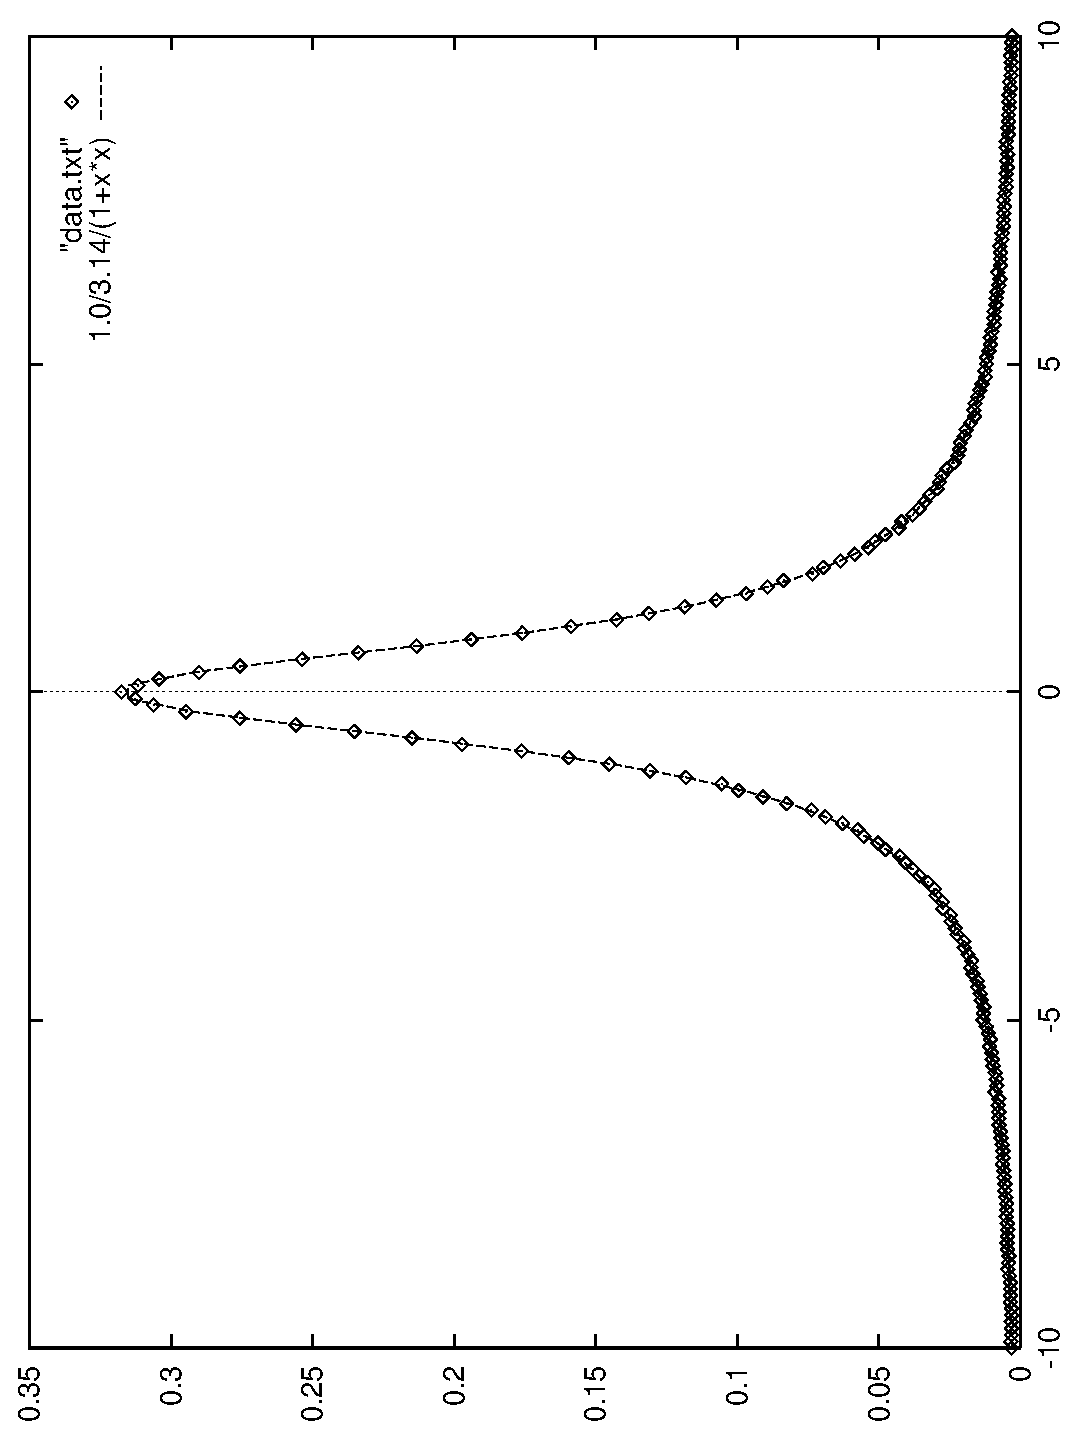
\includegraphics[height=12cm]{i-result-cauchy.eps}}\\
\vspace*{10mm}
Fig. A-2-1. The Cauchy distribution.\\
\end{center}

\vspace*{20mm}

\noindent
{\Large A-2-2. Sample Program 7 (Log Normal)}
\addcontentsline{toc}{subsection}{A-2-2. Sample Program 7}
\index{LogNormal}

\vspace*{7mm}

\noindent
The equation for the Log Normal distribution is as follows.

\begin{equation}
f(x) = \left\{
\begin{array}{ll}
\frac{1}{\sqrt{2\pi} \sigma x} \cdot \exp \left\{ \frac{-(\log x - \mu )^2}{2 \sigma^2} \right\} & x>0 \\
0 & x \le 0
\end{array}
\right.
\end{equation}

\noindent
Here,

\begin{equation}
\mu = \log \left( \frac{\mu_{log}^2}{\sqrt{\mu_{log}^2 +
\sigma_{log}^2}} \right)
\end{equation}

\begin{equation}
\sigma = \sqrt{\log \left( \frac{\mu_{log}^2+\sigma_{log}^2}{\mu_{log}^2} \right)}
\end{equation}

\noindent
In the program, I used 

\begin{equation}
\mu_{log} = \sqrt{e}
\end{equation}

\clearpage

\begin{equation}
\sigma_{log}^2 = e (e-1)
\end{equation}

\vspace*{5mm}

\noindent
The next program is a sample for the Log Normal distribution.

\vspace*{10mm}

{\footnotesize
\begin{center}
\begin{tabular}{|l|}\hline
\#include "Population.h"\\
\#include $<$fstream.h$>$\\
\#include $<$stdio.h$>$\\
\#include $<$LogNormal.h$>$\\
\hspace*{\textwidth}\\
void main(void)\\
\{\\
\\
\hspace*{10mm}// declaration\\
\hspace*{10mm}int seed      = 1234;\\
\hspace*{10mm}int i,j;\\
\hspace*{10mm}int total     = 1000000;\\
\hspace*{10mm}double r;\\
\hspace*{10mm}double rstore[total];\\
\hspace*{10mm}double start  = -0.005;\\
\hspace*{10mm}double end    = 10.005;\\
\hspace*{10mm}int div       =   1001;\\
\hspace*{10mm}double step   = (end-start)/div;\\
\hspace*{10mm}int counter[div];\\
\hspace*{10mm}double position[div];\\
\\
\hspace*{10mm}// instantialize\\
\hspace*{10mm}LogNormal lognormal;\\
\\
\hspace*{10mm}// initialization\\
\hspace*{10mm}for (i=0;i$<$div;i++)\{\\
\hspace*{20mm}counter[i]=0;\\
\hspace*{10mm}\}\\
\\
\hspace*{10mm}// file open\\
\hspace*{10mm}FILE *fp;\\
\hspace*{10mm}fp = fopen("data.txt","w");\\
\\
\hspace*{10mm}// random seed\\
\hspace*{10mm}Rng::seed(seed);\\\hline
\end{tabular}
\vspace*{5mm}

{\small
Example 7. Sample Program 7-1.
}
\end{center}
}

\clearpage

{\footnotesize
\begin{center}
\begin{tabular}{|l|}\hline
\hspace*{10mm}// random generator\\
\hspace*{10mm}for (i=0;i$<$total;i++)\{\\
\hspace*{20mm}lognormal.mean(SqrtE);\\
\hspace*{20mm}lognormal.variance(E*(E-1));\\
\hspace*{20mm}r = lognormal();\\
\hspace*{20mm}rstore[i]=r;\\
\hspace*{20mm}for (j=0;j$<$div;j++)\{\\
\hspace*{30mm}position[j] = start + (j+j+1)*step/2.0;\\
\hspace*{30mm}if (r$>$=start+j*step \&\& r<start+(j+1)*step)\{\\
\hspace*{40mm}++counter[j];\\
\hspace*{30mm}\}\\
\hspace*{20mm}\}\\
\hspace*{10mm}\}\\
\\
\hspace*{10mm}// output\\
\hspace*{10mm}double prob;\\
\hspace*{10mm}for (j=0;j$<$div;j++)\{\\
\hspace*{20mm}prob = static\_cast$<$double$>$(counter[j]) / static\_cast$<$double$>$(total)/step;\\
\hspace*{20mm}fprintf(fp,"\%f \%f $\backslash$n",position[j],prob);\\
\hspace*{10mm}\}\\
\hspace*{\textwidth}\\
\}\\\hline
\end{tabular}
\vspace*{5mm}

{\small
Example 7. Sample Program 7-2.
}
\end{center}
}

\vspace*{10mm}

\noindent
The result of this program is shown in the next figure.

\clearpage

\begin{center}
\rotatebox{-90}{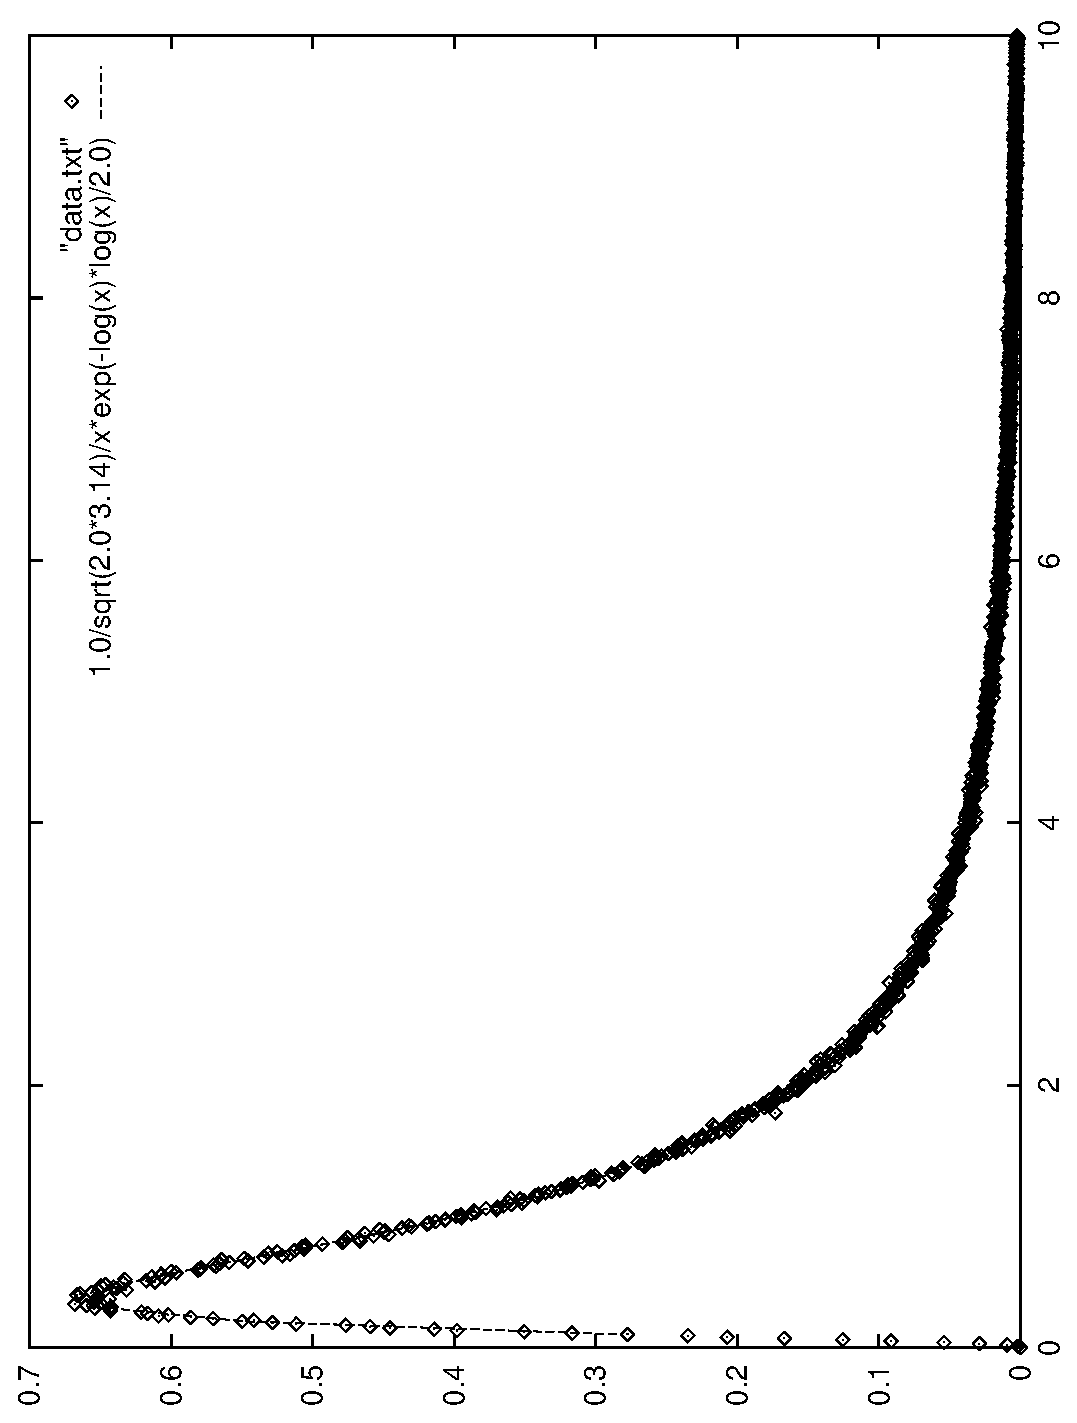
\includegraphics[height=12cm]{i-result-lognormal.eps}}\\
\vspace*{10mm}
Fig. A-2-2. The Log Normal distribution.\\
\end{center}

\vspace*{20mm}

\noindent
{\Large A-2-3. Sample Program 8 (Normal)}
\addcontentsline{toc}{subsection}{A-2-3. Sample Program 8}
\index{Normal}

\vspace*{7mm}

\noindent
The equation for the Normal distribution is as follows.

\begin{equation}
f(x) = \frac{1}{\sqrt{2\pi}\sigma} \cdot \exp{\frac{-(x-\mu)^2}{2\sigma^2}}
\end{equation}

\noindent
In the program, I used

\begin{equation}
\mu = 3 \hspace{3mm} , \hspace{3mm} \sigma^2 = 4
\end{equation}

\vspace*{5mm}

\noindent
The next program is a sample for the Normal distribution.

\clearpage

{\footnotesize
\begin{center}
\begin{tabular}{|l|}\hline
\#include "Population.h"\\
\#include $<$fstream.h$>$\\
\#include $<$stdio.h$>$\\
\hspace*{\textwidth}\\
void main(void)\\
\{\\
\\
\hspace*{10mm}// declaration\\
\hspace*{10mm}int seed      = 1234;\\
\hspace*{10mm}int i,j;\\
\hspace*{10mm}int total     = 1000000;\\
\hspace*{10mm}double r;\\
\hspace*{10mm}double rstore[total];\\
\hspace*{10mm}double start  = -3.006;\\
\hspace*{10mm}double end    =  9.006;\\
\hspace*{10mm}int div       =   1001;\\
\hspace*{10mm}double step   = (end-start)/div;\\
\hspace*{10mm}int counter[div];\\
\hspace*{10mm}double position[div];\\
\\
\hspace*{10mm}// initialization\\
\hspace*{10mm}for (i=0;i$<$div;i++)\{\\
\hspace*{20mm}counter[i]=0;\\
\hspace*{10mm}\}\\
\\
\hspace*{10mm}// file open\\
\hspace*{10mm}FILE *fp;\\
\hspace*{10mm}fp = fopen("data.txt","w");\\
\\
\hspace*{10mm}// random seed\\
\hspace*{10mm}Rng::seed(seed);\\
\\
\hspace*{10mm}// random generator\\
\hspace*{10mm}for (i=0;i$<$total;i++)\{\\
\hspace*{20mm}Rng::gauss.mean(3.0);\\
\hspace*{20mm}Rng::gauss.variance(4.0);\\
\hspace*{20mm}r = Rng::gauss();\\
\hspace*{20mm}rstore[i]=r;\\
\hspace*{20mm}for (j=0;j$<$div;j++)\{\\
\hspace*{30mm}position[j] = start + (j+j+1)*step/2.0;\\
\hspace*{30mm}if (r$>$=start+j*step \&\& r<start+(j+1)*step)\{\\
\hspace*{40mm}++counter[j];\\
\hspace*{30mm}\}\\
\hspace*{20mm}\}\\
\hspace*{10mm}\}\\\hline
\end{tabular}
\vspace*{5mm}

{\small
Example 8. Sample Program 8-1.
}
\end{center}
}

\clearpage

{\footnotesize
\begin{center}
\begin{tabular}{|l|}\hline
\hspace*{10mm}// output\\
\hspace*{10mm}double prob;\\
\hspace*{10mm}for (j=0;j$<$div;j++)\{\\
\hspace*{20mm}prob = static\_cast$<$double$>$(counter[j]) / static\_cast$<$double$>$(total)/step;\\
\hspace*{20mm}fprintf(fp,"\%f \%f $\backslash$n",position[j],prob);\\
\hspace*{10mm}\}\\
\hspace*{\textwidth}\\
\}\\\hline
\end{tabular}
\vspace*{5mm}

{\small
Example 8. Sample Program 8-2.
}
\end{center}
}

\vspace*{10mm}

\noindent
The result of this program is shown in the next figure.

\vspace*{10mm}

\begin{center}
\rotatebox{-90}{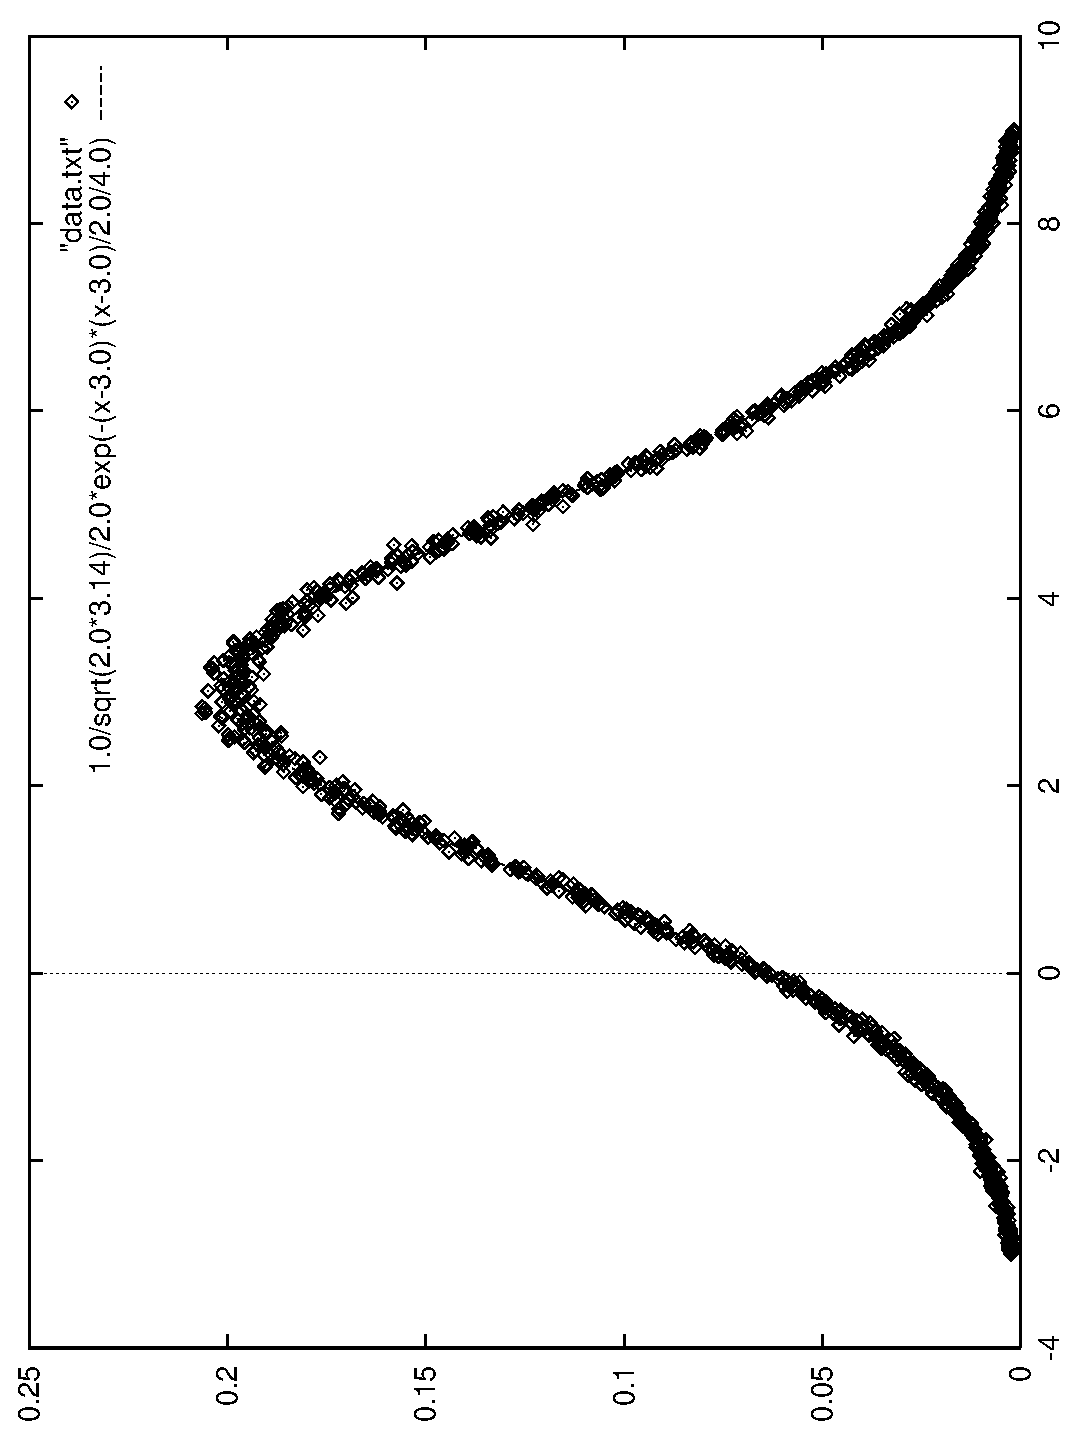
\includegraphics[height=12cm]{i-result-normal.eps}}\\
\vspace*{10mm}
Fig. A-2-3. The Normal distribution.\\
\end{center}

\clearpage

\noindent
{\Large A-2-4. Sample Program 9 (Uniform)}
\addcontentsline{toc}{subsection}{A-2-4. Sample Program 9}
\index{Uniform}

\vspace*{7mm}

\noindent
The equation for the Uniform distribution is as follows.

\begin{equation}
f(x) = \left\{
\begin{array}{ll}
1 / ( x_{upper} - x_{lower} )  & x_{lower} \le x \le x_{upper} \\
0 & the \hspace{2mm} other
\end{array}
\right.
\end{equation}

\noindent
In the program, I used

\begin{equation}
x_{lower} = 1.0 \hspace{3mm} , \hspace{3mm} x_{upper} = 2.0
\end{equation}

\vspace*{5mm}

\noindent
The next program is a sample for the Uniform distribution.

\vspace*{10mm}

{\footnotesize
\begin{center}
\begin{tabular}{|l|}\hline
\#include "Population.h"\\
\#include $<$fstream.h$>$\\
\#include $<$stdio.h$>$\\
\hspace*{\textwidth}\\
void main(void)\\
\{\\
\\
\hspace*{10mm}// declaration\\
\hspace*{10mm}int seed      = 1234;\\
\hspace*{10mm}int i,j;\\
\hspace*{10mm}int total     = 1000000;\\
\hspace*{10mm}double r;\\
\hspace*{10mm}double rstore[total];\\
\hspace*{10mm}double start  = 1.0;\\
\hspace*{10mm}double end    = 2.0;\\
\hspace*{10mm}int div       = 1000;\\
\hspace*{10mm}double step   = (end-start)/div;\\
\hspace*{10mm}int counter[div];\\
\hspace*{10mm}double position[div];\\
\\
\hspace*{10mm}// initialization\\
\hspace*{10mm}for (i=0;i$<$div;i++)\{\\
\hspace*{20mm}counter[i]=0;\\
\hspace*{10mm}\}\\\hline
\end{tabular}
\vspace*{5mm}

{\small
Example 9. Sample Program 9-1.
}
\end{center}
}  

\clearpage

{\footnotesize
\begin{center}
\begin{tabular}{|l|}\hline
\hspace*{10mm}// file open\\
\hspace*{10mm}FILE *fp;\\
\hspace*{10mm}fp = fopen("data.txt","w");\\
\\
\hspace*{10mm}// random seed\\
\hspace*{10mm}Rng::seed(seed);\\
\\
\hspace*{10mm}// random generator\\
\hspace*{10mm}for (i=0;i$<$total;i++)\{\\
\hspace*{20mm}Rng::uni.low(start);\\
\hspace*{20mm}Rng::uni.high(end);\\
\hspace*{20mm}r = Rng::uni();\\
\hspace*{20mm}rstore[i]=r;\\
\hspace*{20mm}for (j=0;j$<$div;j++)\{\\
\hspace*{30mm}position[j] = start + (j+j+1)*step/2.0;\\
\hspace*{30mm}if (r$>$=start+j*step \&\& r<start+(j+1)*step)\{\\
\hspace*{40mm}++counter[j];\\
\hspace*{30mm}\}\\
\hspace*{20mm}\}\\
\hspace*{10mm}\}\\
\\
\hspace*{10mm}// output\\
\hspace*{10mm}double prob;\\
\hspace*{10mm}for (j=0;j$<$div;j++)\{\\
\hspace*{20mm}prob = static\_cast$<$double$>$(counter[j]) / static\_cast$<$double$>$(total)/step;\\
\hspace*{20mm}fprintf(fp,"\%f \%f $\backslash$n",position[j],prob);\\
\hspace*{10mm}\}\\
\\
\}\\\hline
\end{tabular}
\vspace*{5mm}

{\small
Example 9. Sample Program 9-2.
}
\end{center}
}  

\vspace*{5mm}

\noindent
The result of this program is shown in the next figure.

\clearpage

\begin{center}
\rotatebox{-90}{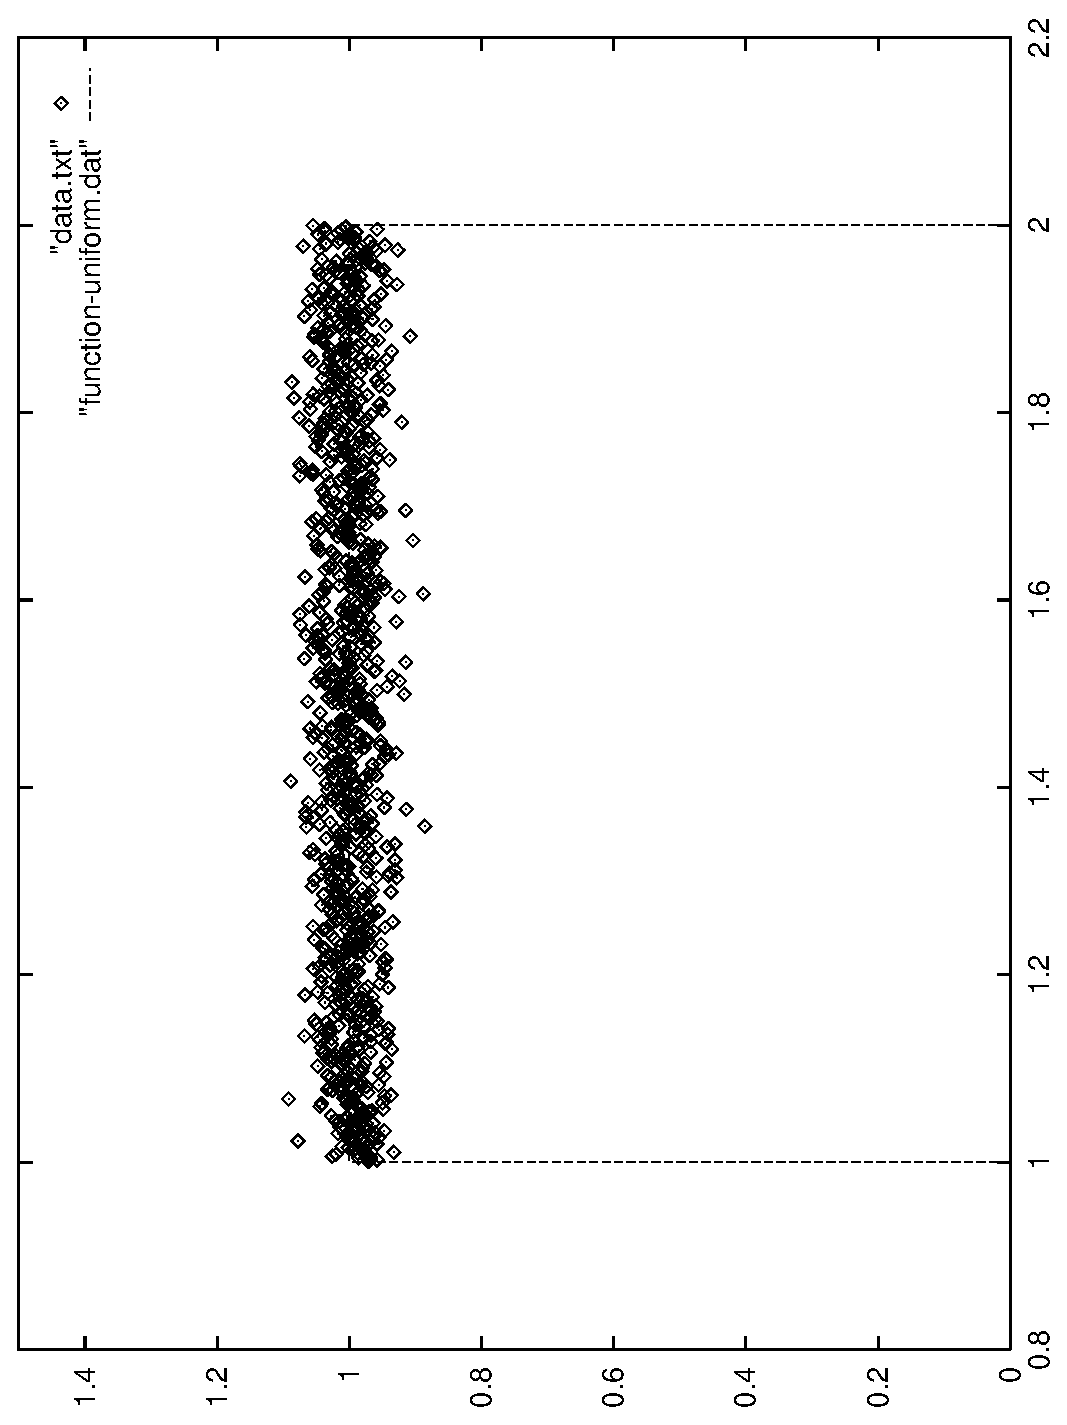
\includegraphics[height=12cm]{i-result-uniform.eps}}\\
\vspace*{10mm}
Fig. A-2-4. The Uniform distribution.\\
\end{center}

\vspace*{20mm}

\noindent
{\Large A-2-5. Sample Program 10 (Weibull)}
\addcontentsline{toc}{subsection}{A-2-5. Sample Program 10}
\index{Weibull}

\vspace*{7mm}

\noindent
The equation for the Weibull distribution is as follows.

\begin{equation}
f(x) = \frac{\alpha}{\beta} \cdot \exp \left\{ - \frac{1}{\beta} x^\alpha \right\} \cdot x^{\alpha-1}
\end{equation}

\noindent
In the program, I used

\begin{equation}
\alpha = 2  \hspace{3mm} , \hspace{3mm} \beta = 3
\end{equation}

\vspace*{5mm}

\noindent
The next program is a sample for the Weibull distribution.

\clearpage

{\footnotesize
\begin{center}
\begin{tabular}{|l|}\hline
\#include "Population.h"\\
\#include $<$fstream.h$>$\\
\#include $<$stdio.h$>$\\
\#include $<$Weibull.h$>$\\
\hspace*{\textwidth}\\
void main(void)\\
\{\\
\\
\hspace*{10mm}// declaration\\
\hspace*{10mm}int seed      = 1234;\\
\hspace*{10mm}int i,j;\\
\hspace*{10mm}int total     = 1000000;\\
\hspace*{10mm}double r;\\
\hspace*{10mm}double rstore[total];\\
\hspace*{10mm}double start  = -0.005;\\
\hspace*{10mm}double end    = 10.005;\\
\hspace*{10mm}int div       = 1001;\\
\hspace*{10mm}double step   = (end-start)/div;\\
\hspace*{10mm}int counter[div];\\
\hspace*{10mm}double position[div];\\
\\
\hspace*{10mm}// instantialize\\
\hspace*{10mm}Weibull weibull;\\
\\
\hspace*{10mm}// initialization\\
\hspace*{10mm}for (i=0;i$<$div;i++)\{\\
\hspace*{20mm}counter[i]=0;\\
\hspace*{10mm}\}\\
\\
\hspace*{10mm}// file open\\
\hspace*{10mm}FILE *fp;\\
\hspace*{10mm}fp = fopen("data.txt","w");\\
\\
\hspace*{10mm}// random seed\\
\hspace*{10mm}Rng::seed(seed);\\
\hspace*{10mm}// random generator\\
\hspace*{10mm}for (i=0;i$<$total;i++)\{\\
\hspace*{20mm}weibull.alpha(2.0);\\
\hspace*{20mm}weibull.beta(3.0);\\
\hspace*{20mm}r = weibull();\\
\hspace*{20mm}rstore[i]=r;\\
\hspace*{20mm}for (j=0;j$<$div;j++)\{\\
\hspace*{30mm}position[j] = start + (j+j+1)*step/2.0;\\
\hspace*{30mm}if (r$>$=start+j*step \&\& r$<$start+(j+1)*step)\{\\
\hspace*{40mm}++counter[j];\\\hline
\end{tabular}
\vspace*{5mm}

{\small
Example 10. Sample Program 10-1.
}
\end{center}
}  

\clearpage

  
{\footnotesize
\begin{center}
\begin{tabular}{|l|}\hline

\hspace*{30mm}\}\\
\hspace*{20mm}\}\\
\hspace*{10mm}\}\\
\\
\hspace*{10mm}// output\\
\hspace*{10mm}double prob;\\
\hspace*{10mm}for (j=0;j$<$div;j++)\{\\
\hspace*{20mm}prob = static\_cast$<$double$>$(counter[j]) / static\_cast$<$double$>$(total)/step;\\
\hspace*{20mm}fprintf(fp,"\%f \%f $\backslash$n",position[j],prob);\\
\hspace*{10mm}\}\\
\hspace*{\textwidth}\\
\}\\\hline
\end{tabular}
\vspace*{5mm}

{\small
Example 10. Sample Program 10-2.
}
\end{center}
}  
  
\vspace*{5mm}

\noindent
The result of this program is shown in the next figure.

\vspace*{5mm}

\begin{center}
\rotatebox{-90}{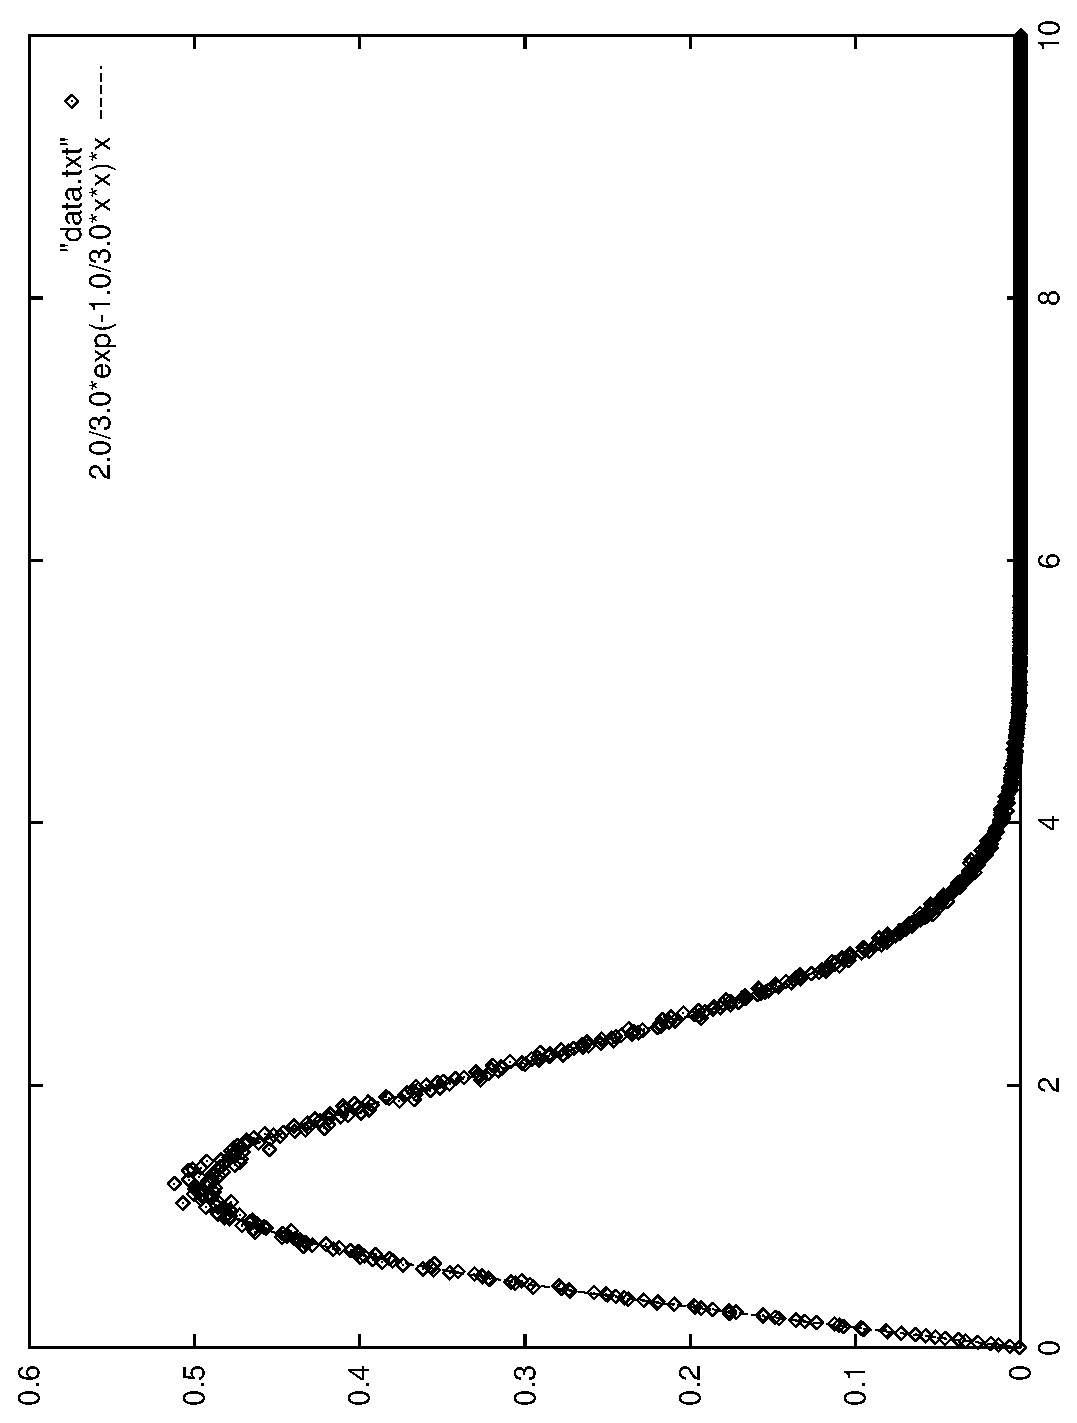
\includegraphics[height=12cm]{i-result-weibull.eps}}\\
\vspace*{10mm}
Fig. A-2-5. Weibull distribution.\\
\end{center}







%************************************************************************
% Bibliography
%************************************************************************
\clearpage
\addcontentsline{toc}{chapter}{Bibliography}
\begin{thebibliography}{55}
 
    \bibitem{Foundations}
    {\em Foundations of Genetic Algorithms}, G.J.E. Rawlings (Editor),
    Morgan Kaufmann Publishers, San Mateo, CA, 1991.

    \bibitem{ICEC96}
    {\em Proceedings of the 1996 IEEE Internal Conference on Evolutionary 
    Computation (ICEC '96)}.
   
    \bibitem{First}
    {\em Proceedings of the First International Conference on Genetic 
    Algorithms and Their Applications} (ICGA 1985), published by
    J.J. Grefenstette, Pittsburgh, PA, Juli 24-26 1985, Carnegie-Mellon 
    University, Lawrence Erlbaum Associates (Hillsdale, NJ, 1988).

    \bibitem{Third}
    {\em Proceedings of the Third International Conference on Genetic 
    Algorithms} (ICGA 1989), published by J.D. Schaffer, July 4-7, 
    San Mateo, CA, 1989, George Mason University, Morgan Kaufmann 
    Publishers Inc.

    \bibitem{Eshelman95}
    {\em Proceedings of the Sixth International Conference on Genetic
    Algorithms}, published by L.J. Eshelman, 1995.

    \bibitem{Goldberg}
    {\em A comparative analysis of selection schemes used in genetic
    algorithms}, by D.E. Goldberg and K. Deb published at pages
    69 to 93 in \cite{Foundations}.

    \bibitem{Baeck}
    {\em Evolutionary Algorithms in Theory and Practice}, 
    dissertation thesis by T. B\"ack, University of Dortmund, 
    Department of Computer Science, February 1994.

    \bibitem{EALibRef}
    {\em EALib: A \cpp\ class library for evolutionary algorithms}, 
    version 1.5, 2000, by M. Kreutz, B. Sendhoff and C. Igel, 
    Institut f\"ur Neuroinformatik, Ruhr-Universit\"at Bochum.

    \bibitem{Baker}
    {\em Adaptive Selection methods for genetic algorithms}, by J.E. Baker, 
    published at the pages 101 to 111 in \cite{First}.

    \bibitem{AlgoWork}
    {\em How genetic algorithms work: A critical look at implicit
    parallelism}, by J.J. Grefenstette and J.E. Baker, published
    at the pages 20 to 27 in \cite{Third}. 

    \bibitem{Whitley}
    {\em The genitor algorithm and selection pressure:
    Why rank-based allocation of reproductive trials is best} by L.D.
    Whitley, published at the pages 116 to 121 in \cite{Third}.

    \bibitem{Fogel}
    {\em Evolutionary Computation: Toward a New Philosophy of
    Machine Intelligence} by D.B. Fogel, IEEE Press, 1995.

    \bibitem{Search}
    {\em Genetic Algorithms in Search, Optimization, and Machine Learning}, 
    by D.E. Goldberg, Addison-Wesley Publishing Company, Inc., Reading, MA, 
    1989.

    \bibitem{Jong}
    {\em An Analysis of the Behaviour of a Class of Genetic Adaptive
    Systems} by K.A.D. Jong, Dept. Computer and Communication Sciences,
    University of Michigan, 1975, Diss. Abstr. Int. 36(10), 5140B,
    University Microfilms No. 76-9381.

    \bibitem{GSA}
    {\em On the Adaptation of Arbitrary Normal Mutation Distributions
    in Evolution Strategies: The Generating Set Adaptation},
    by N. Hansen, A. Ostermeier and A. Gawelczyk, published at the pages
    57 to 64 in \cite{Eshelman95}. 

    \bibitem{CMA}
    {\em Adapting Arbitrary Normal Mutation. Distributions in Evolution
    Strategies: The Covariance Matrix Adaptation}, by N. Hansen and A. 
    Ostermeier, appeared at the pages 312 to 317 in \cite{ICEC96}.

    \bibitem{MSR}
    {\em Schrittweitenadaptation in der Evolutionsstrategie mit einem
    ent\-sto\-chasti\-sier\-ten Ansatz}, by A. Ostermeier, dissertation thesis, 
    Technische Universit\"at Berlin, Fachbereich 6, 1997.

    \bibitem{NRC}
    {\em Numerical Recipes in C ( Second Edition )}, by William
    H. Press, Saul A. Teukolsky, William T. Vettering and Brian
    P. Flannery, Cambridge University Press, 1992. \label{NRC}

\end{thebibliography}



%************************************************************************
% Index
%************************************************************************
\clearpage
\printindex{}


\end{document}






